\section{Experimental work/ analytical investigation/ design}


\subsection{采集数据}
在本实验中,我们使用了预先从生物实验室制备并染色的石蜡包埋组织切片(\ref{label:sample})。使用HM355s自动切片机,按照操作手册,以不同切削角度进行切片,记录切削参数。切片后,组织样本放置于平面上并干燥(\ref{fig:采集样本}),随后在VHX7000显微镜下进行成像,以捕获电子图像数据(\ref{fig:显微镜})。

其中切片机(\autoref{fig:machine})的切片示意图(以牙齿为例) 如\autoref{fig:cutting_machine}所示\cite{4.1}。记录下的切削参数如下:模式设置为连续,进给速度为5.0,修整值为25,速度设定为32,水流速度为7.5,水温约为36摄氏度。切割角度在8到12度之间。

据此,一共得到分辨率为2880*2160的图像数据集。
%在这不要提三个点的鱼的肺泡组织,在后面作为模型二次验证和增强使用。


\begin{figure}[htbp]
    \centering
    \begin{minipage}{0.35\textwidth}
        \centering
        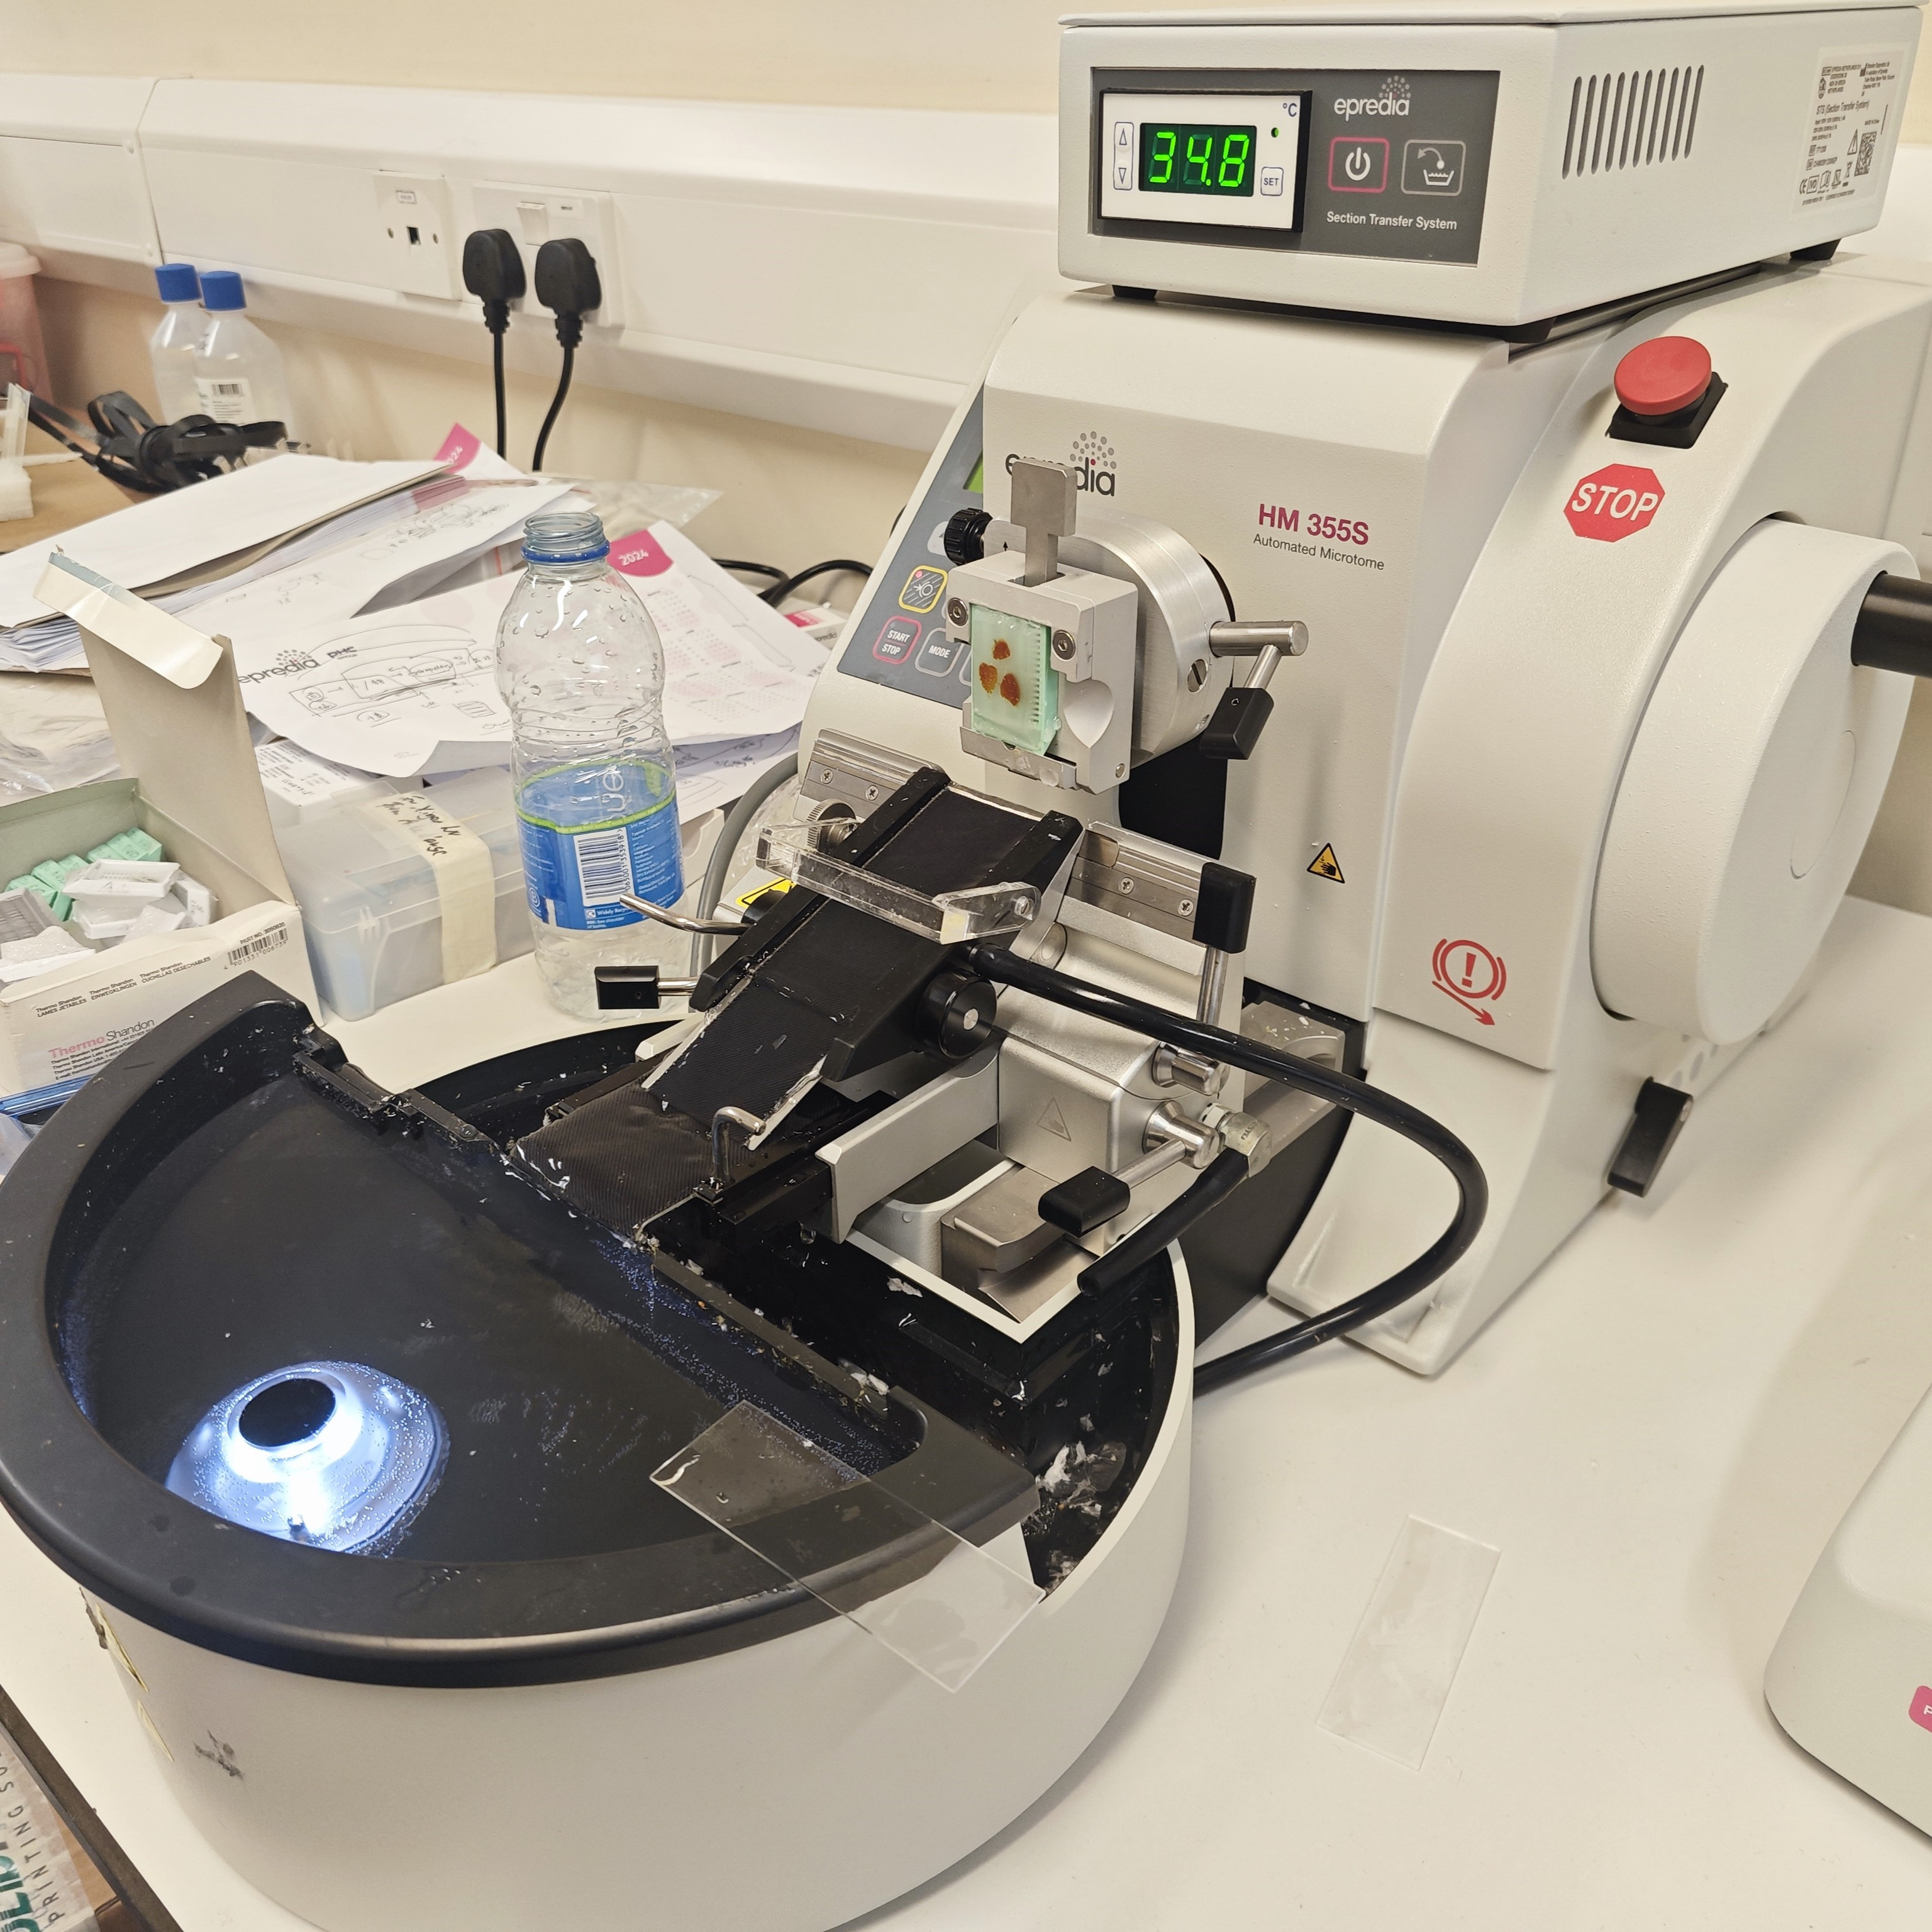
\includegraphics[width=\textwidth]{./fig/machine.jpg}
        \caption{切片机}
        \label{fig:machine}
    \end{minipage}
    \begin{minipage}{0.35\textwidth}
        \centering
        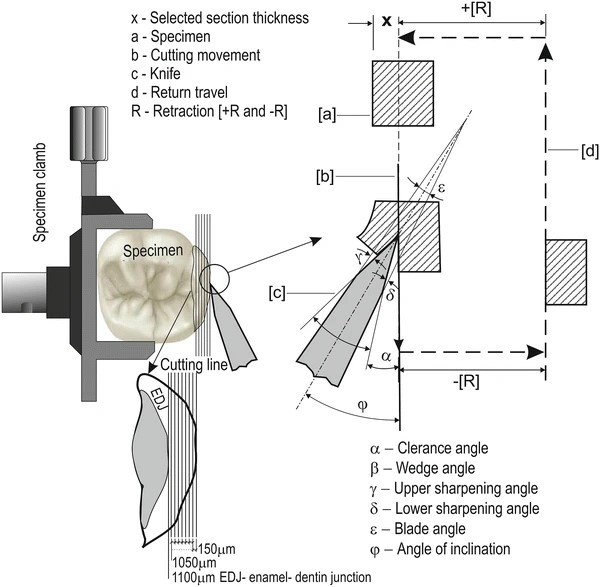
\includegraphics[width=\textwidth]{./fig/10266_2018_353_Fig1_HTML.jpg}
        \caption{切片机示意图}
        \label{fig:cutting_machine}
    \end{minipage}
\end{figure}
% https://link.springer.com/article/10.1007/s10266-018-0353-6


% 在切削过程中,从切角为8度开始(如\autoref{fig:machine}中的angle of inclination),每次增加0.5度,直到切角为12度。切片机在切片过程中保持给进速度为25,厚度为1。

\begin{figure}[htbp]
    \centering
    \begin{minipage}{0.3\textwidth}
        \centering
        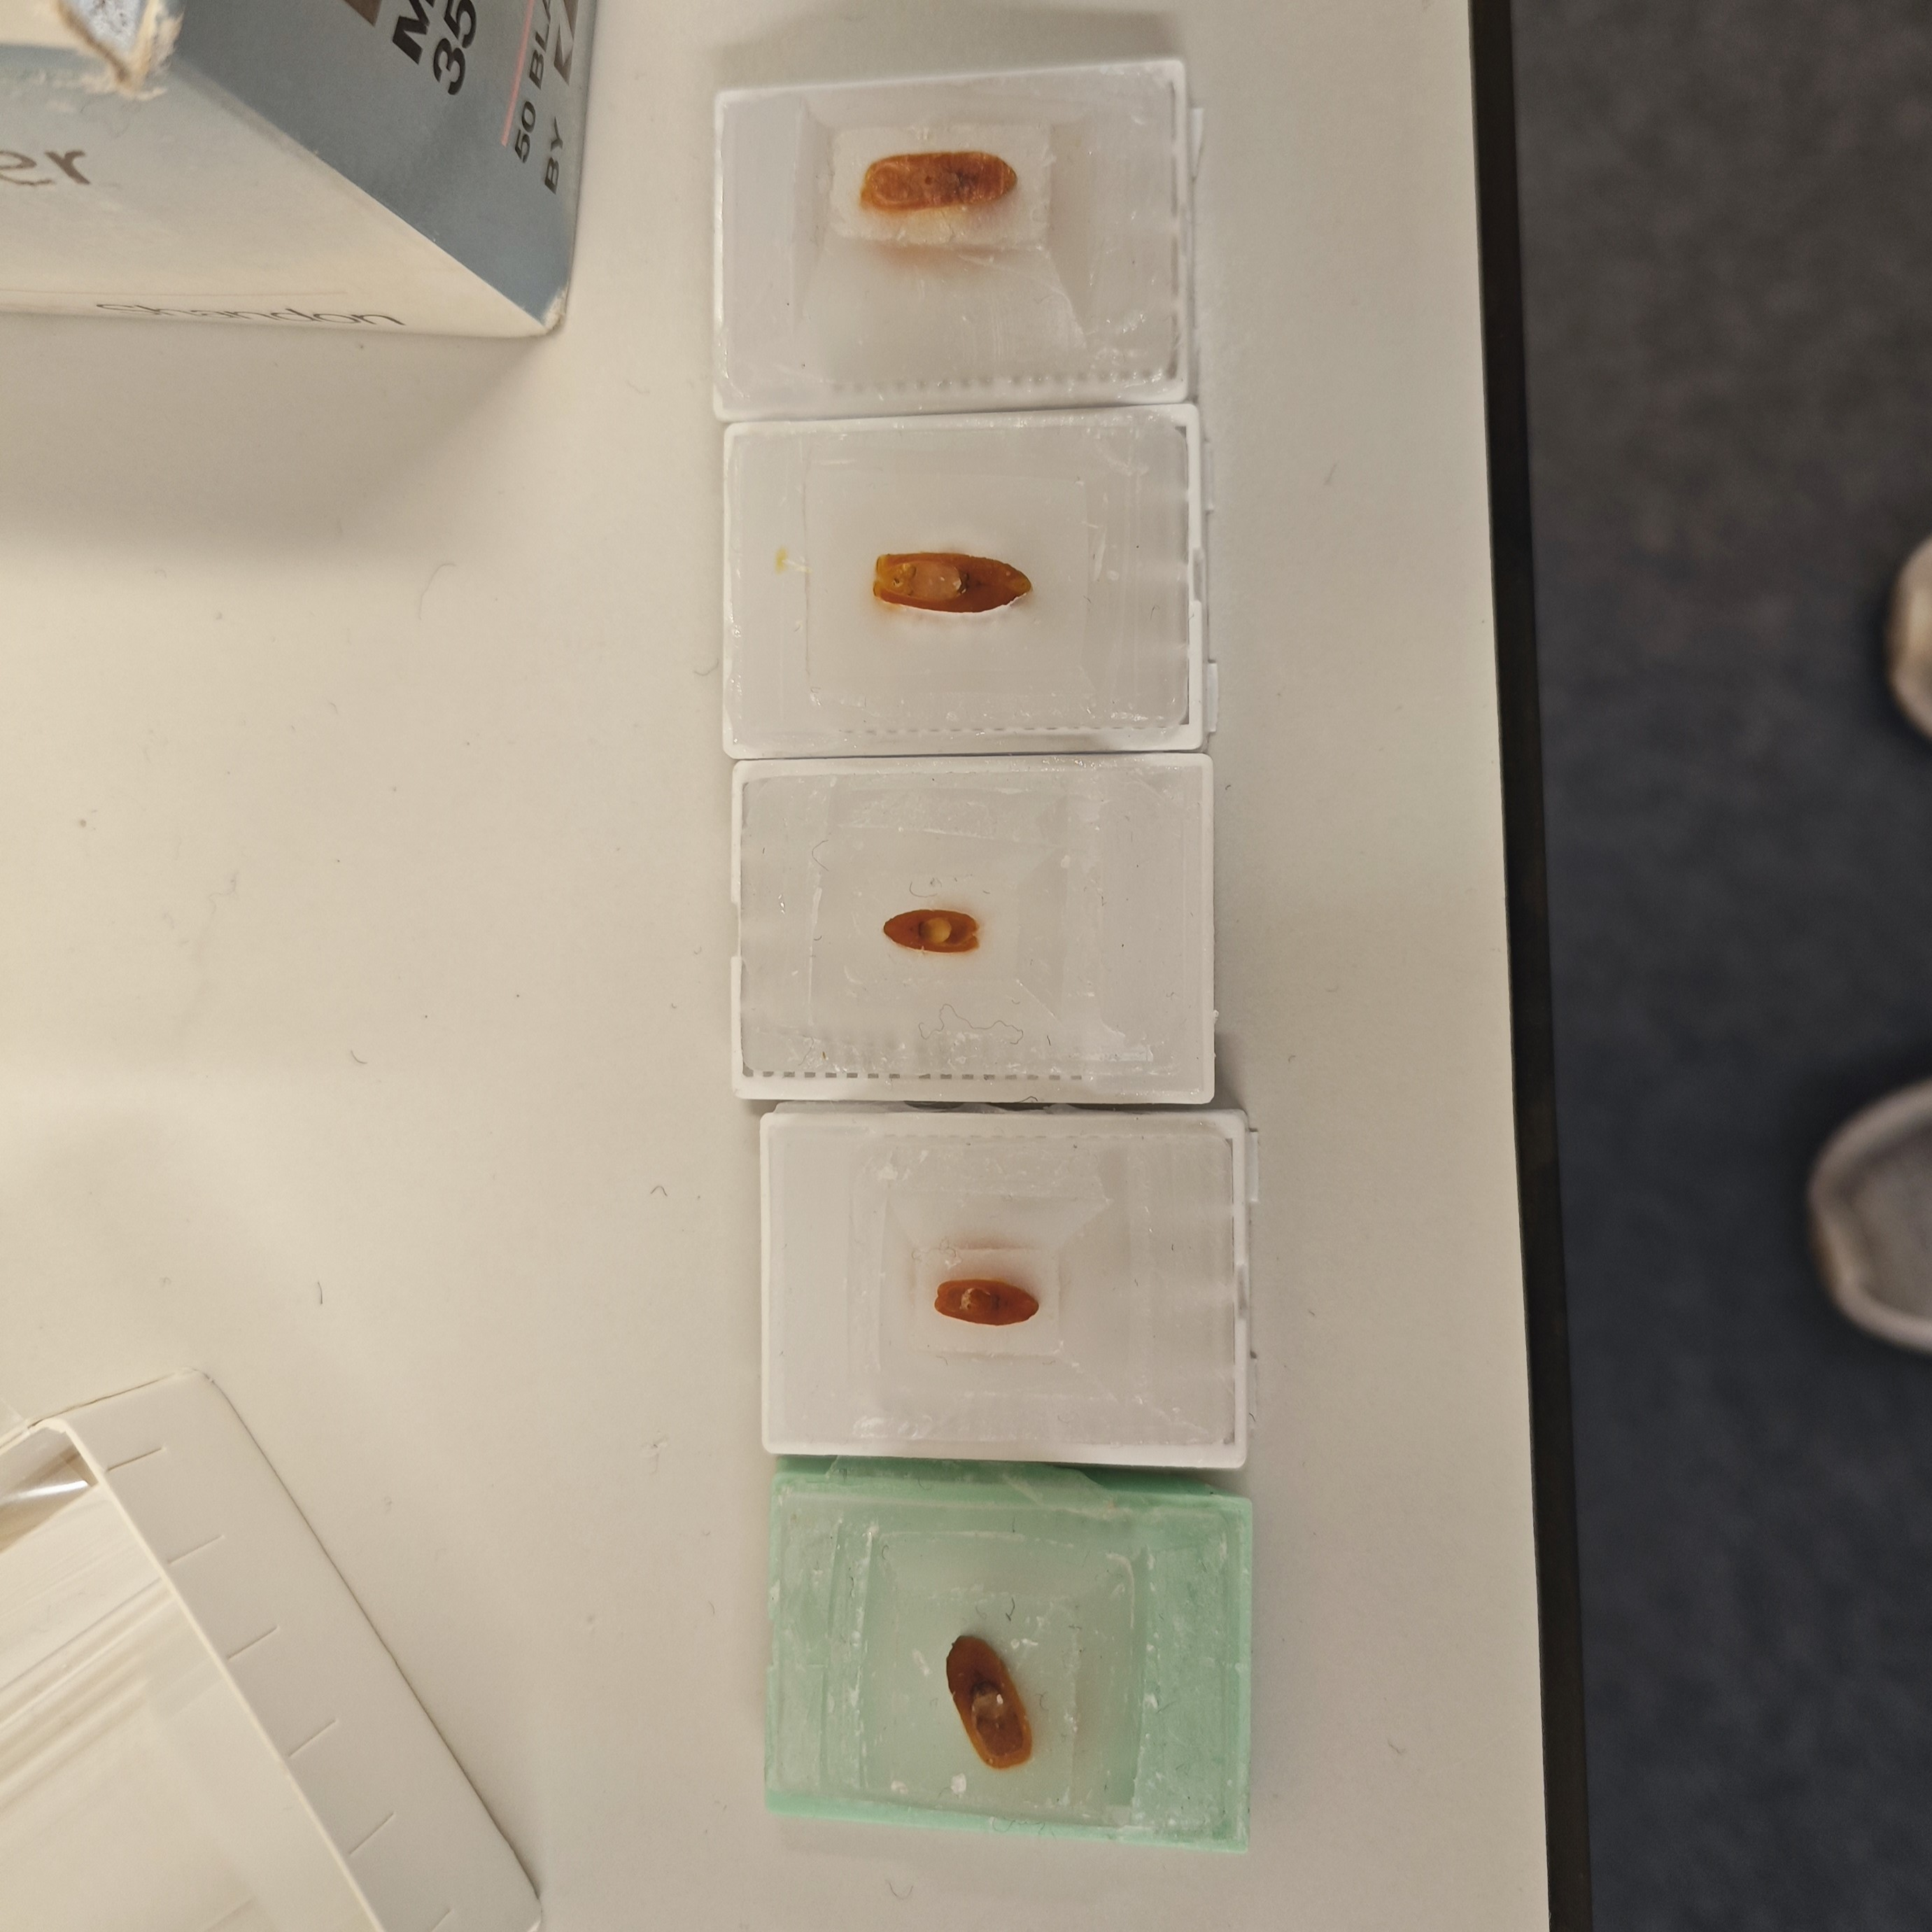
\includegraphics[width=\textwidth]{./fig/sample.jpg}
        \caption{生物组织切片}
        \label{label:sample}
    \end{minipage}
    \begin{minipage}{0.3\textwidth}
        \centering
        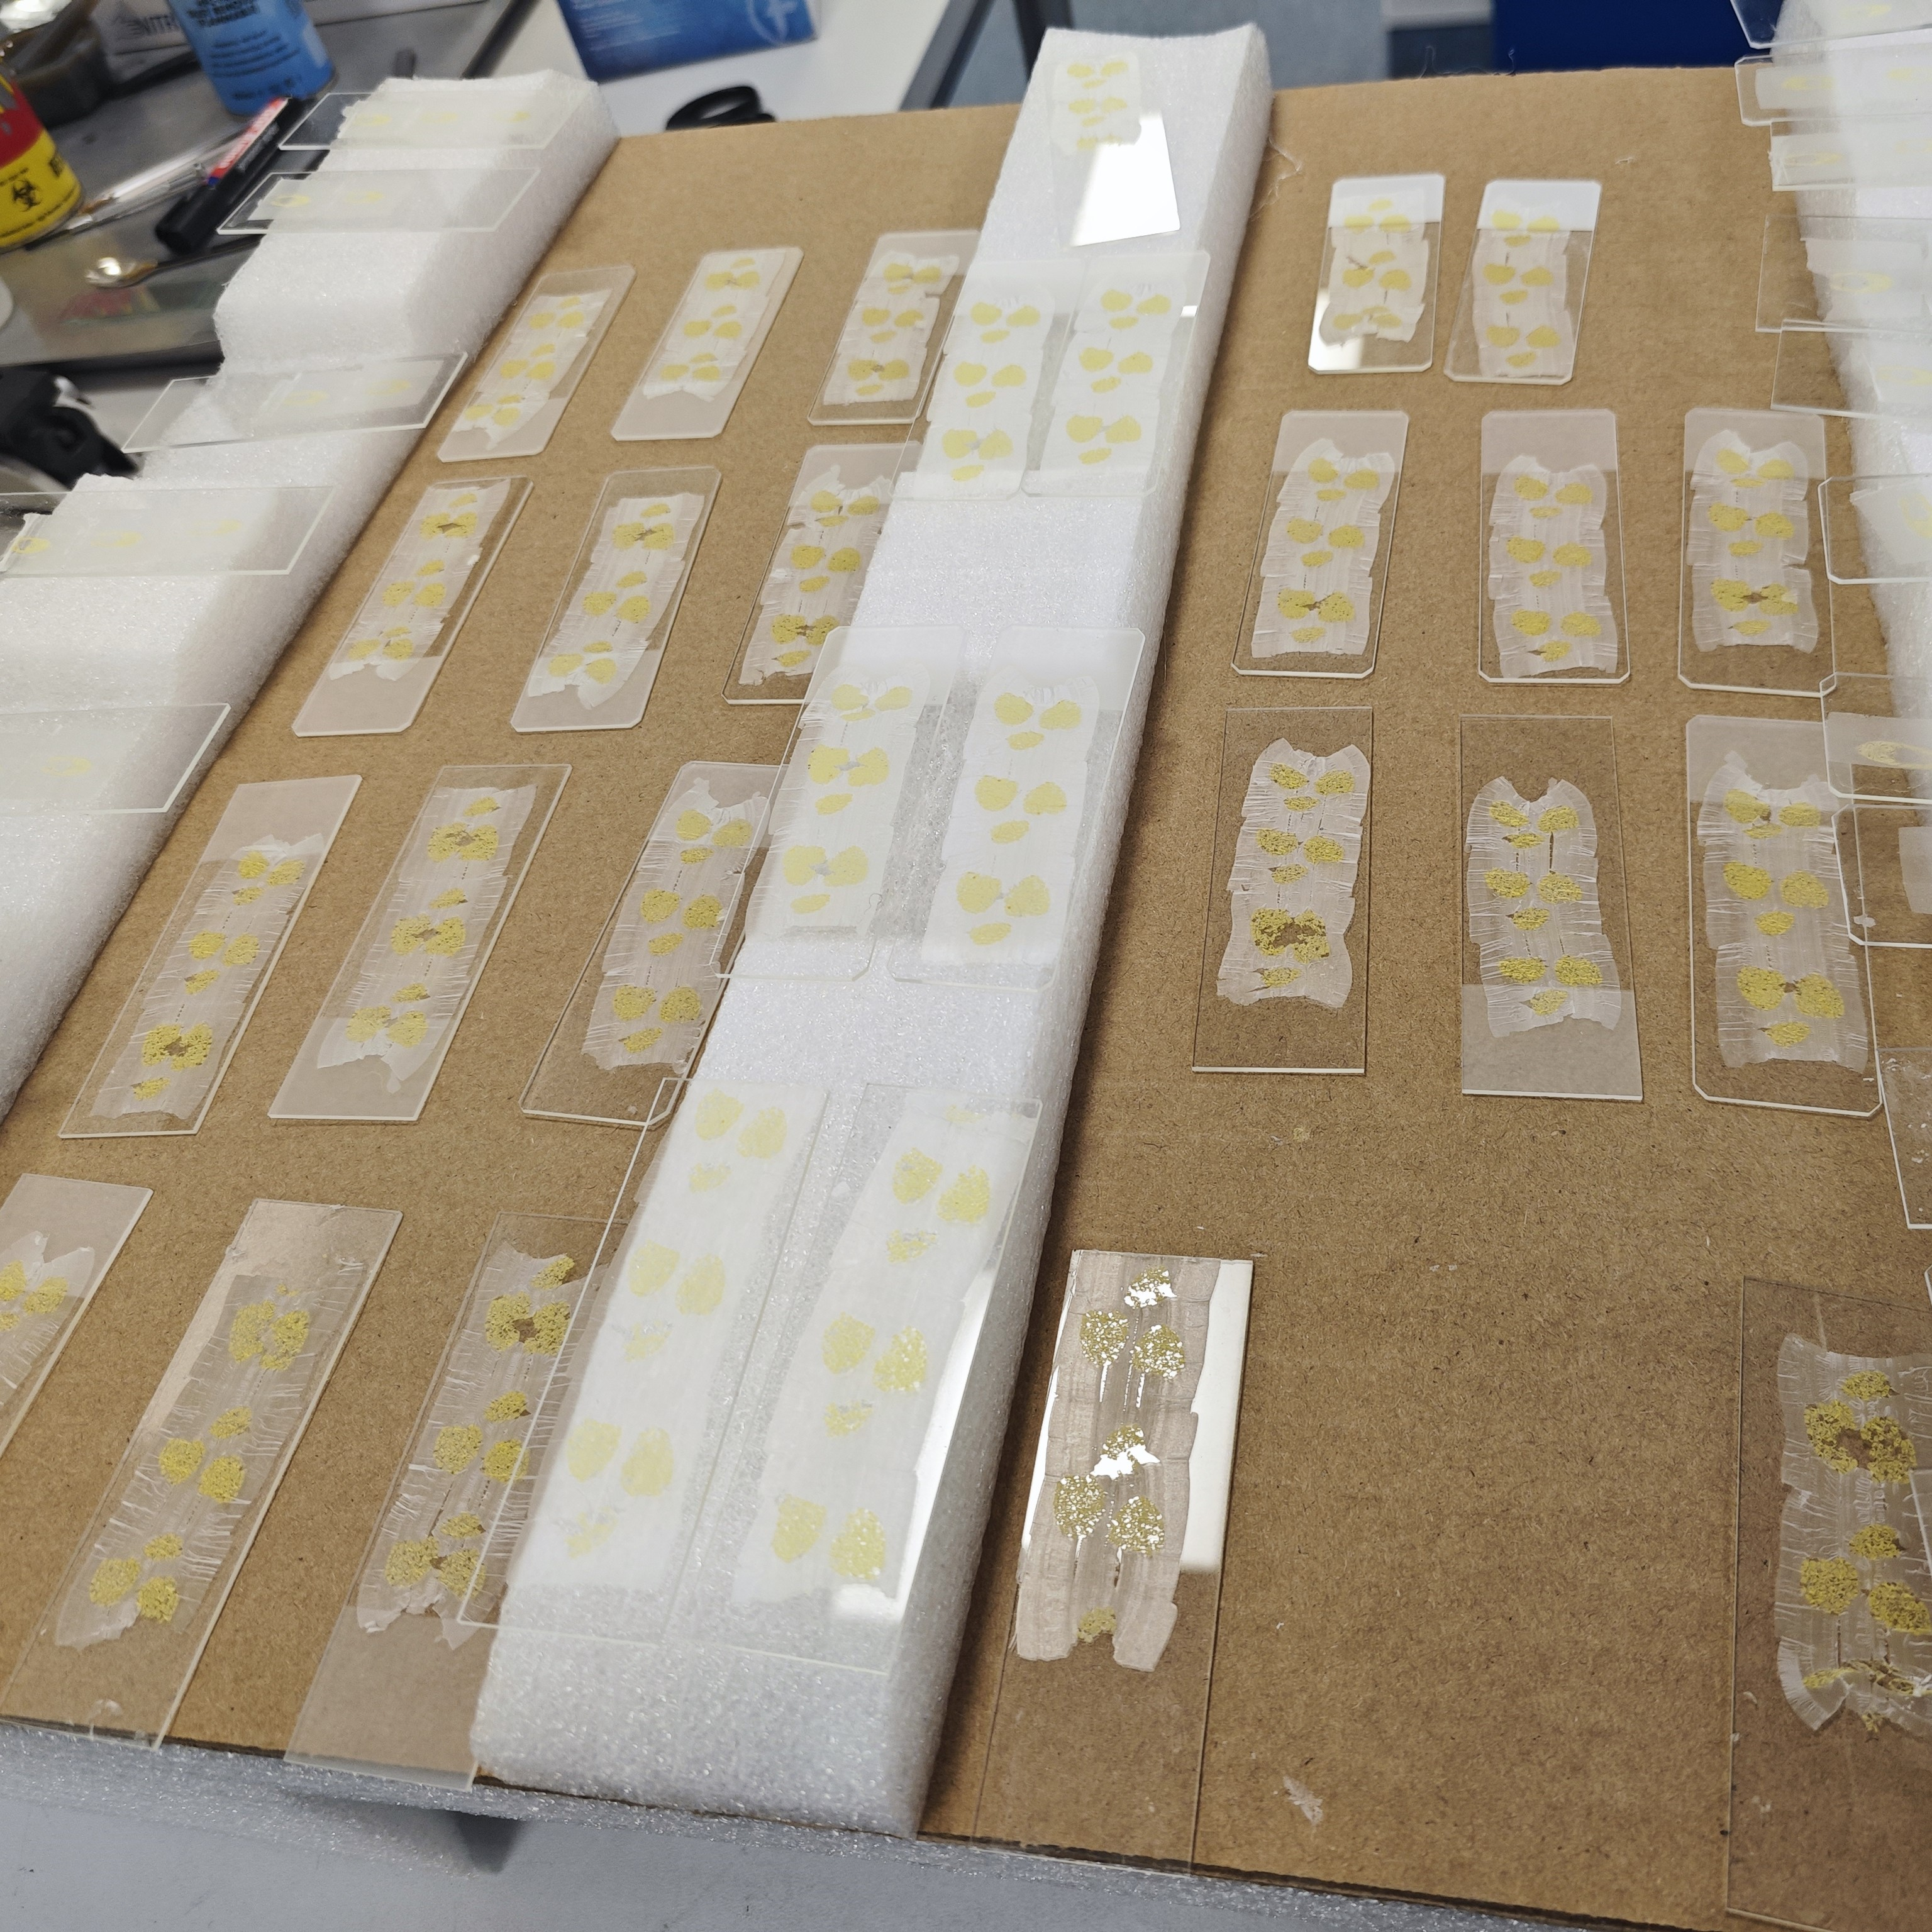
\includegraphics[width=\textwidth]{./fig/采集样本.jpg}
        \caption{采集样本}
        \label{fig:采集样本}
    \end{minipage}
    \begin{minipage}{0.35\textwidth}
        \centering
        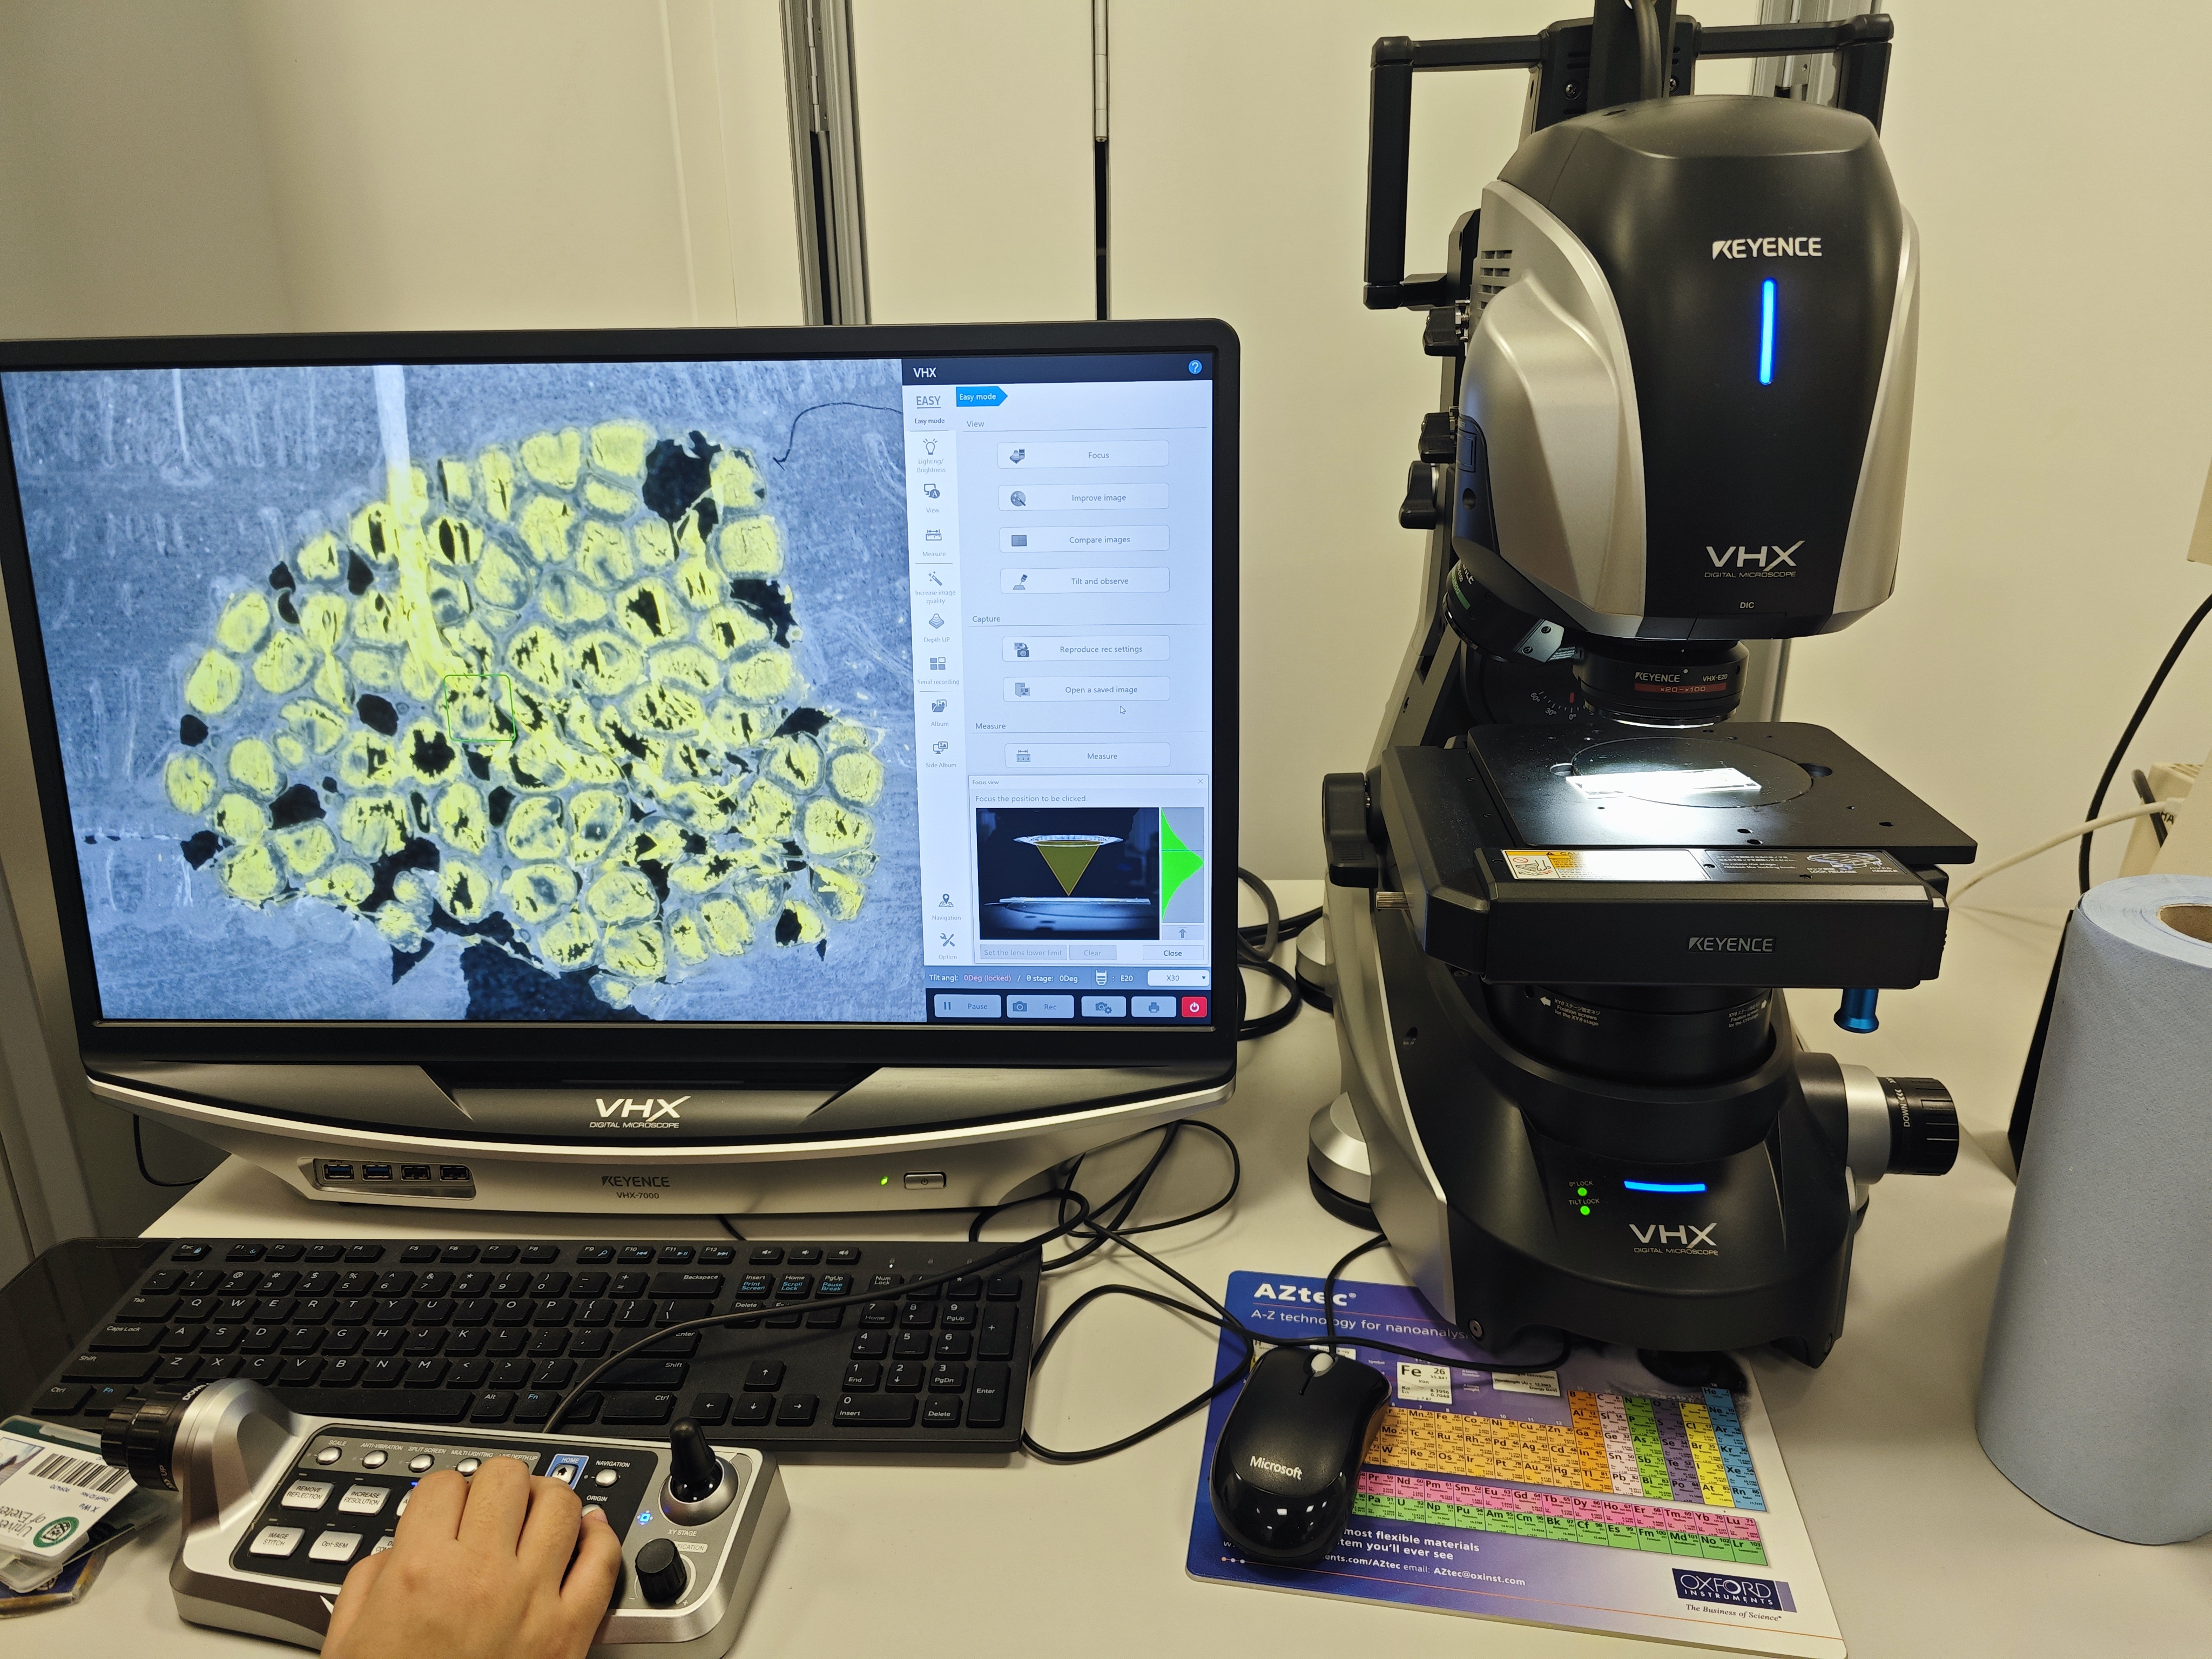
\includegraphics[width=\textwidth]{./fig/显微镜.jpg}
        \caption{显微镜}
        \label{fig:显微镜}
    \end{minipage}
\end{figure}

%图片需要后续更改为卵巢的


% 样本示例如\autoref{fig:sample9.5}所示。

% \begin{figure}
%     \centering
%     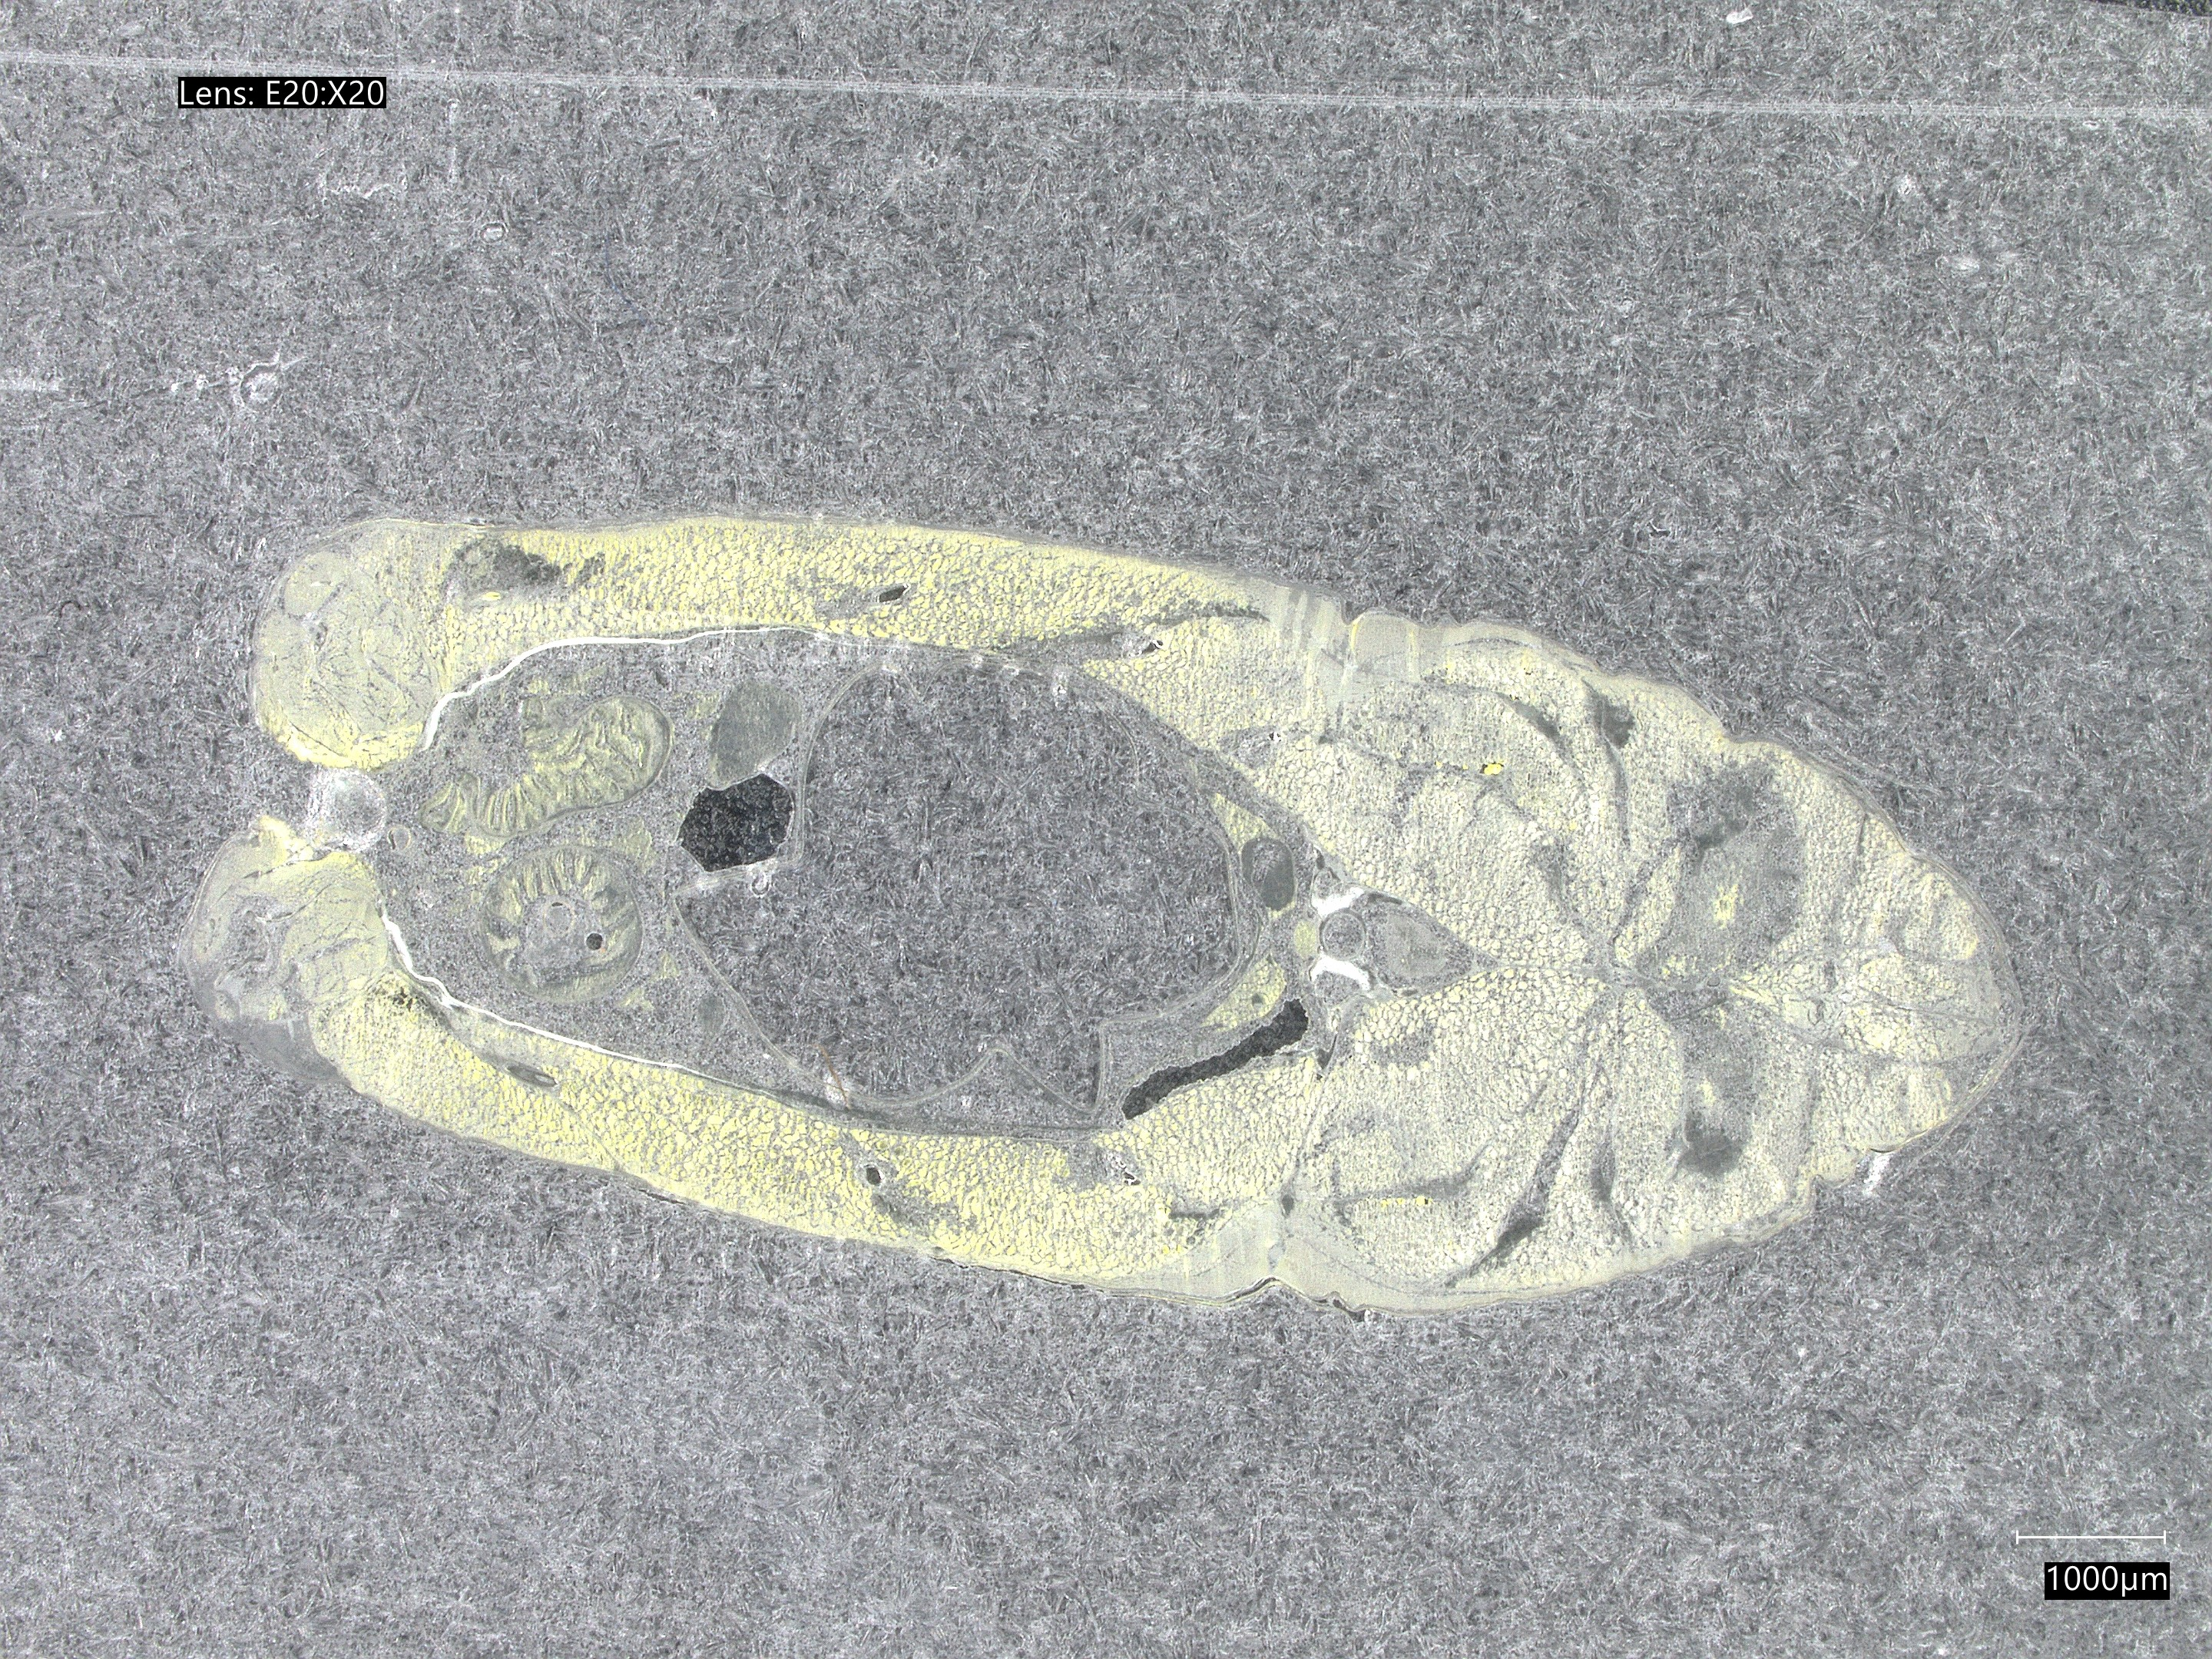
\includegraphics[width=0.8\textwidth]{./fig/sample9.5.jpg}
%     \caption{切角9.5度的样本}
%     \label{fig:sample9.5}
% \end{figure}


\subsection{标注数据}

对于这个实验,数据集是根据组织切片的质量进行标记的。总的来说,生物组织的质量被分为两个主要类别:正常和不良。对收集的数据进行进一步分析,发现了常见的缺陷 - 切片上存在垂直或水平的白色皱纹,这明显表明切片无法使用。鉴于这些缺陷的独特性质,它们被分类为两个额外的特定类别:\textbf{水平线}(见\autoref{fig:horizental_line})和\textbf{垂直线}(见\autoref{fig:vertical_line})。

\begin{figure}[H]
    \centering
    \begin{minipage}{0.33\textwidth}
        \centering
        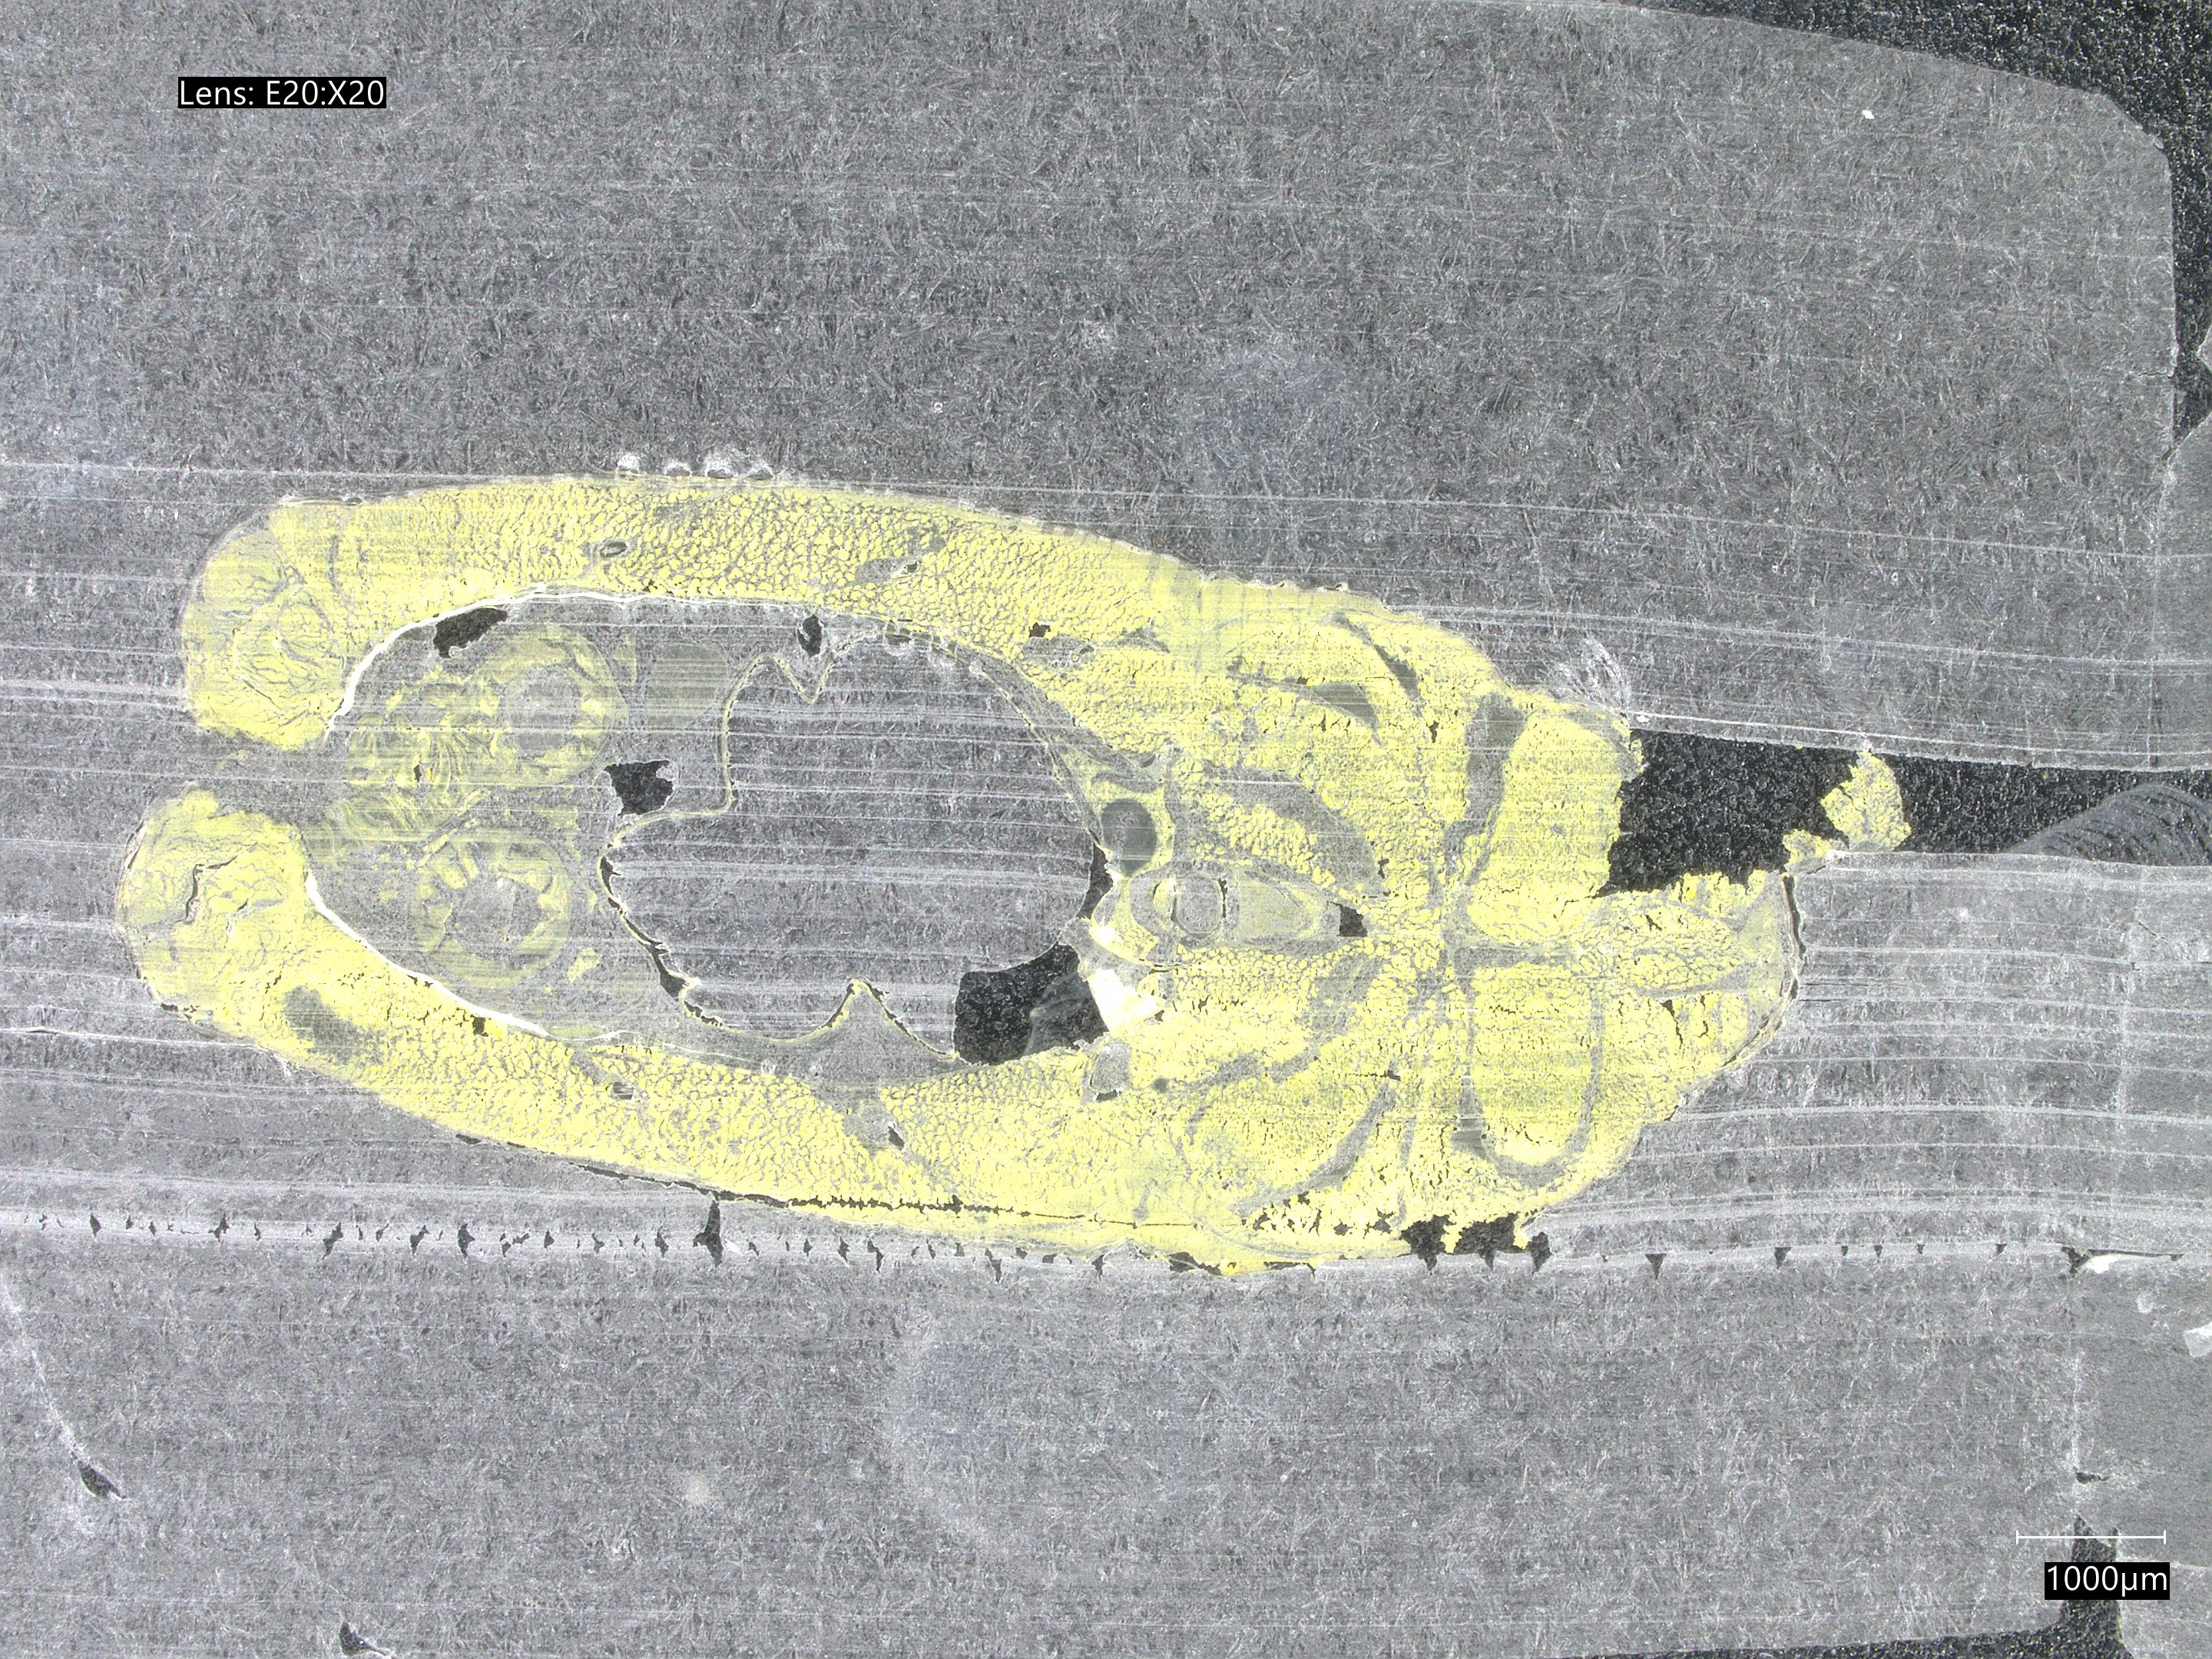
\includegraphics[width=\textwidth]{./fig/sample_1/horizental_line.jpg}
        \caption{horizental line}
        \label{fig:horizental_line}
    \end{minipage}
    \begin{minipage}{0.33\textwidth}
        \centering
        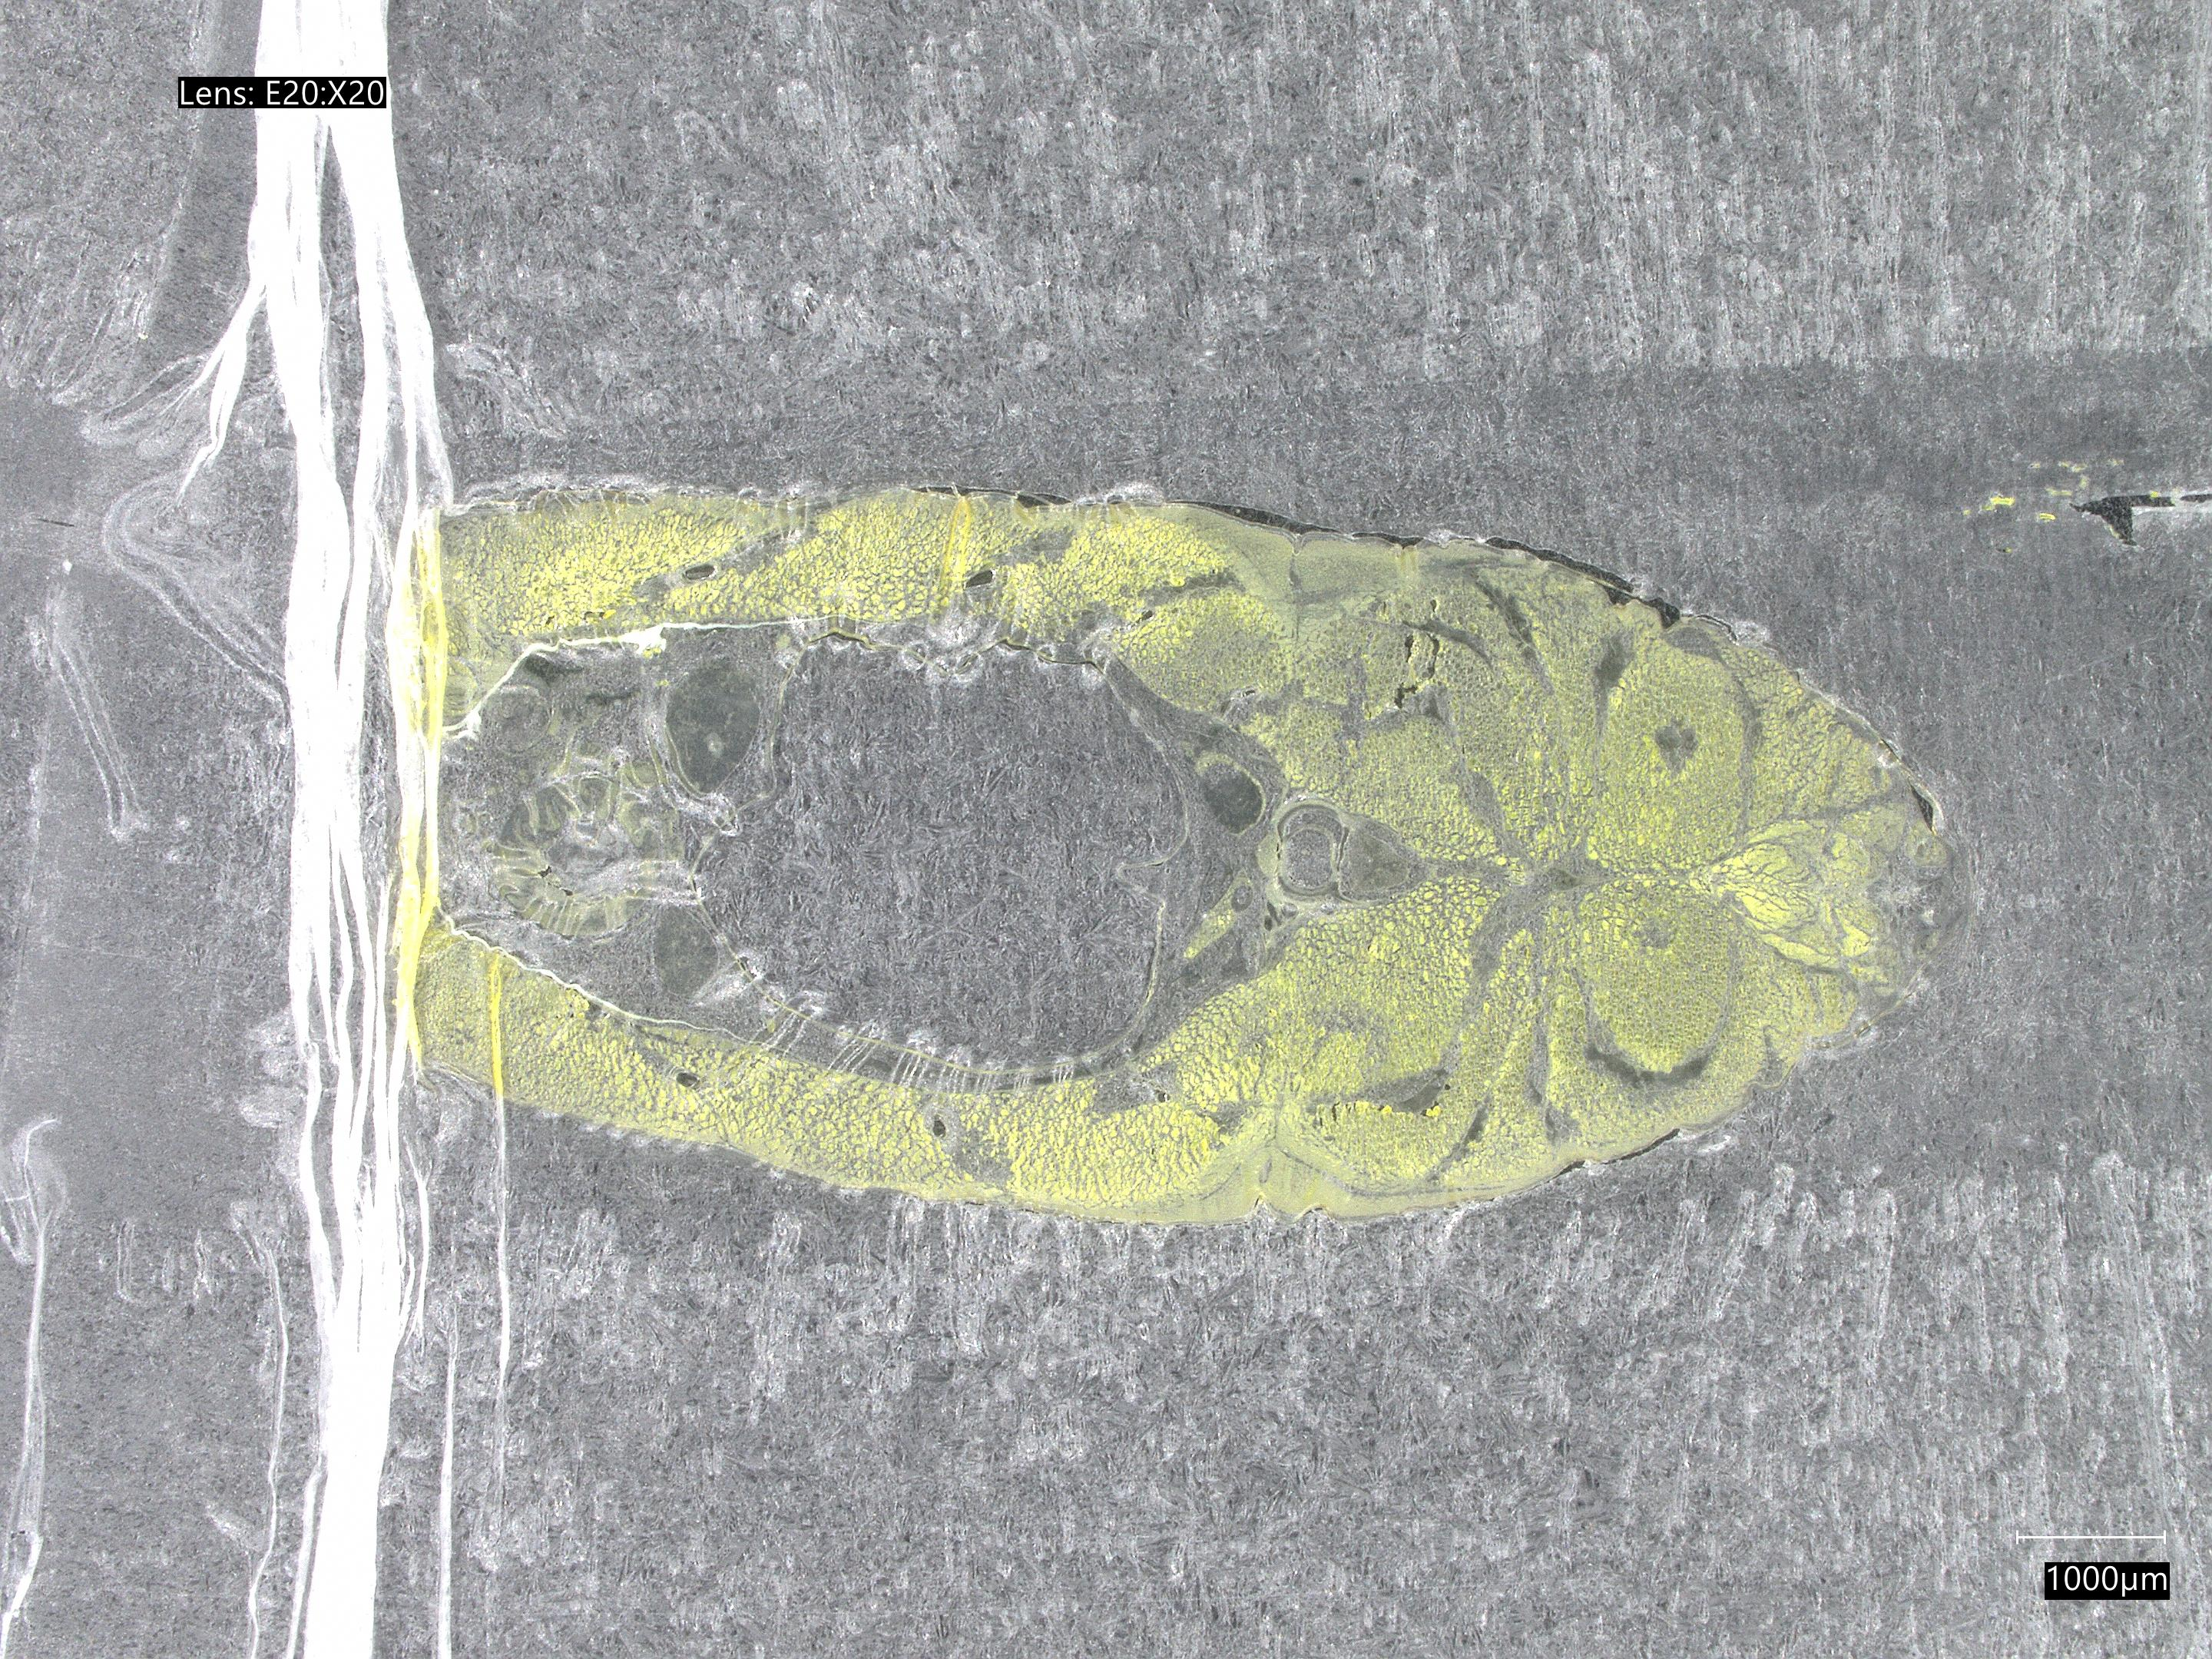
\includegraphics[width=\textwidth]{./fig/sample_1/vertical_line.jpg}
        \caption{vertical line}
        \label{fig:vertical_line}
    \end{minipage}
\end{figure}

此外,考虑到有一部分图片在采样时存在明显的旋转角度,这种情况下,我们也将其单独分为一类,称为slope(如图\autoref{fig:slope})。最后,对于剩下的图片,我们将其标注为other(如图\autoref{fig:other})。

\begin{figure}[H]
    \centering
    \begin{minipage}{0.32\textwidth}
        \centering
        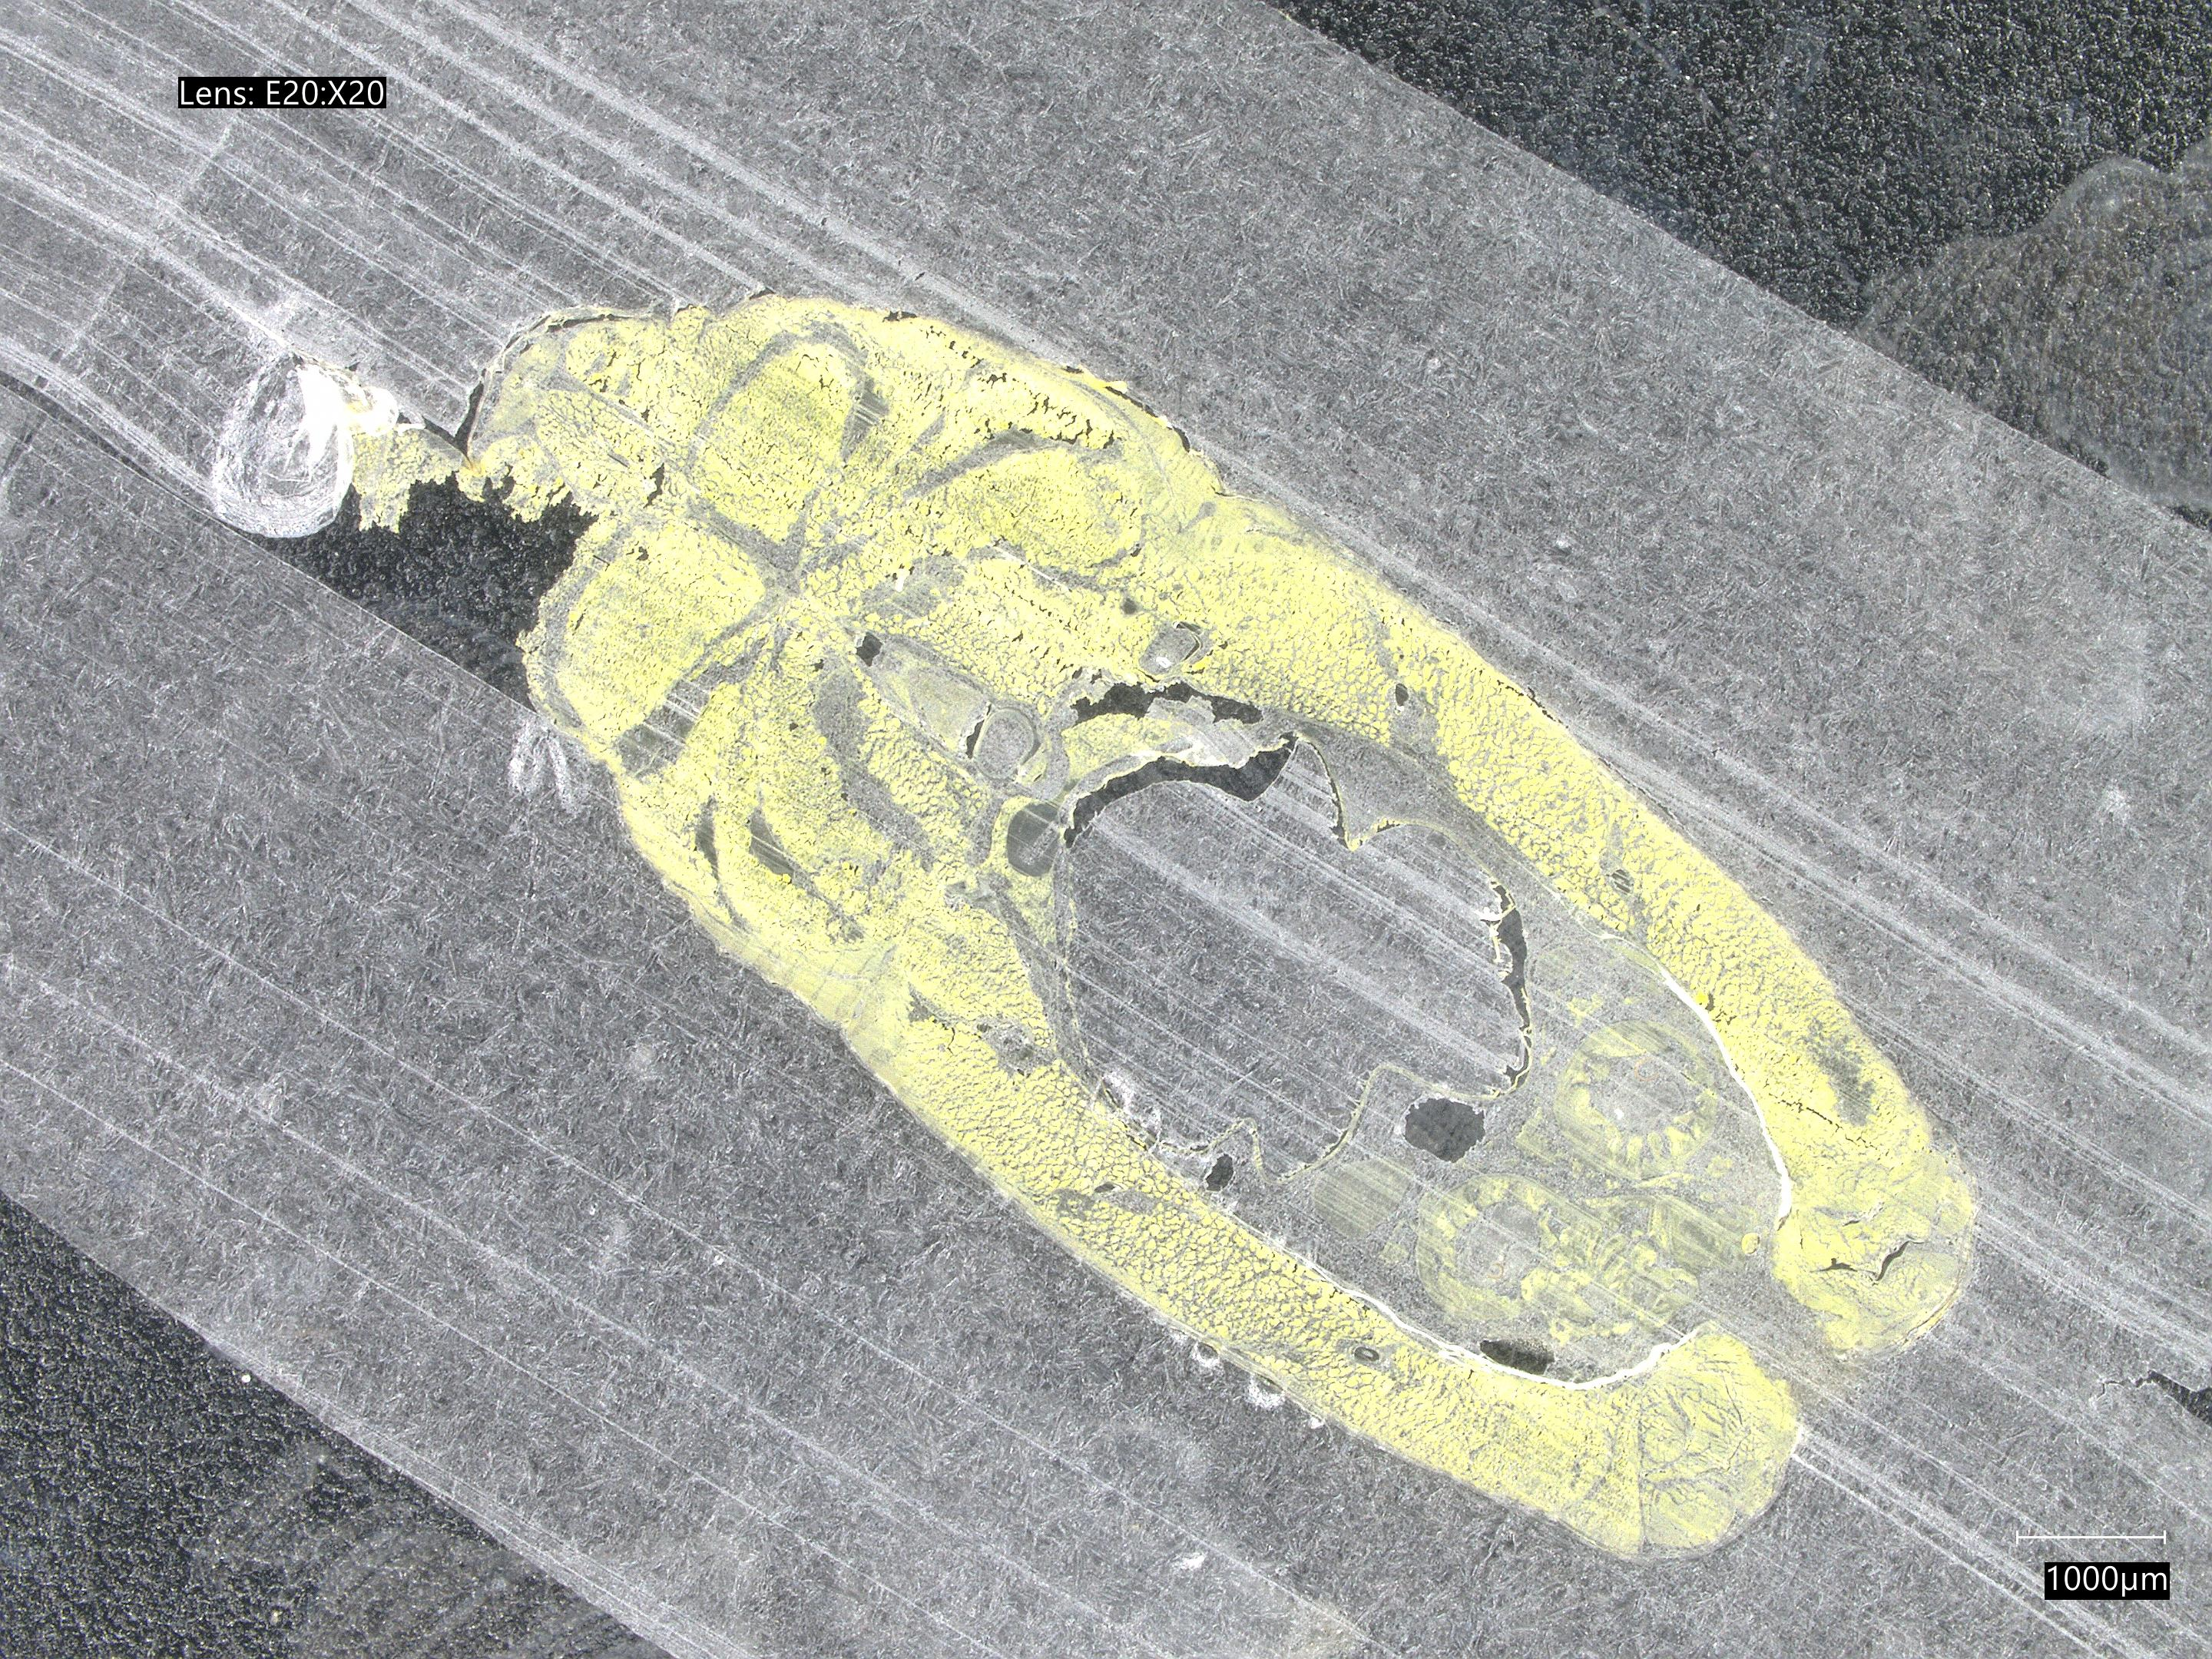
\includegraphics[width=\textwidth]{./fig/sample_1/slope.jpg}
        \caption{slope}
        \label{fig:slope}
    \end{minipage}
    \begin{minipage}{0.32\textwidth}
        \centering
        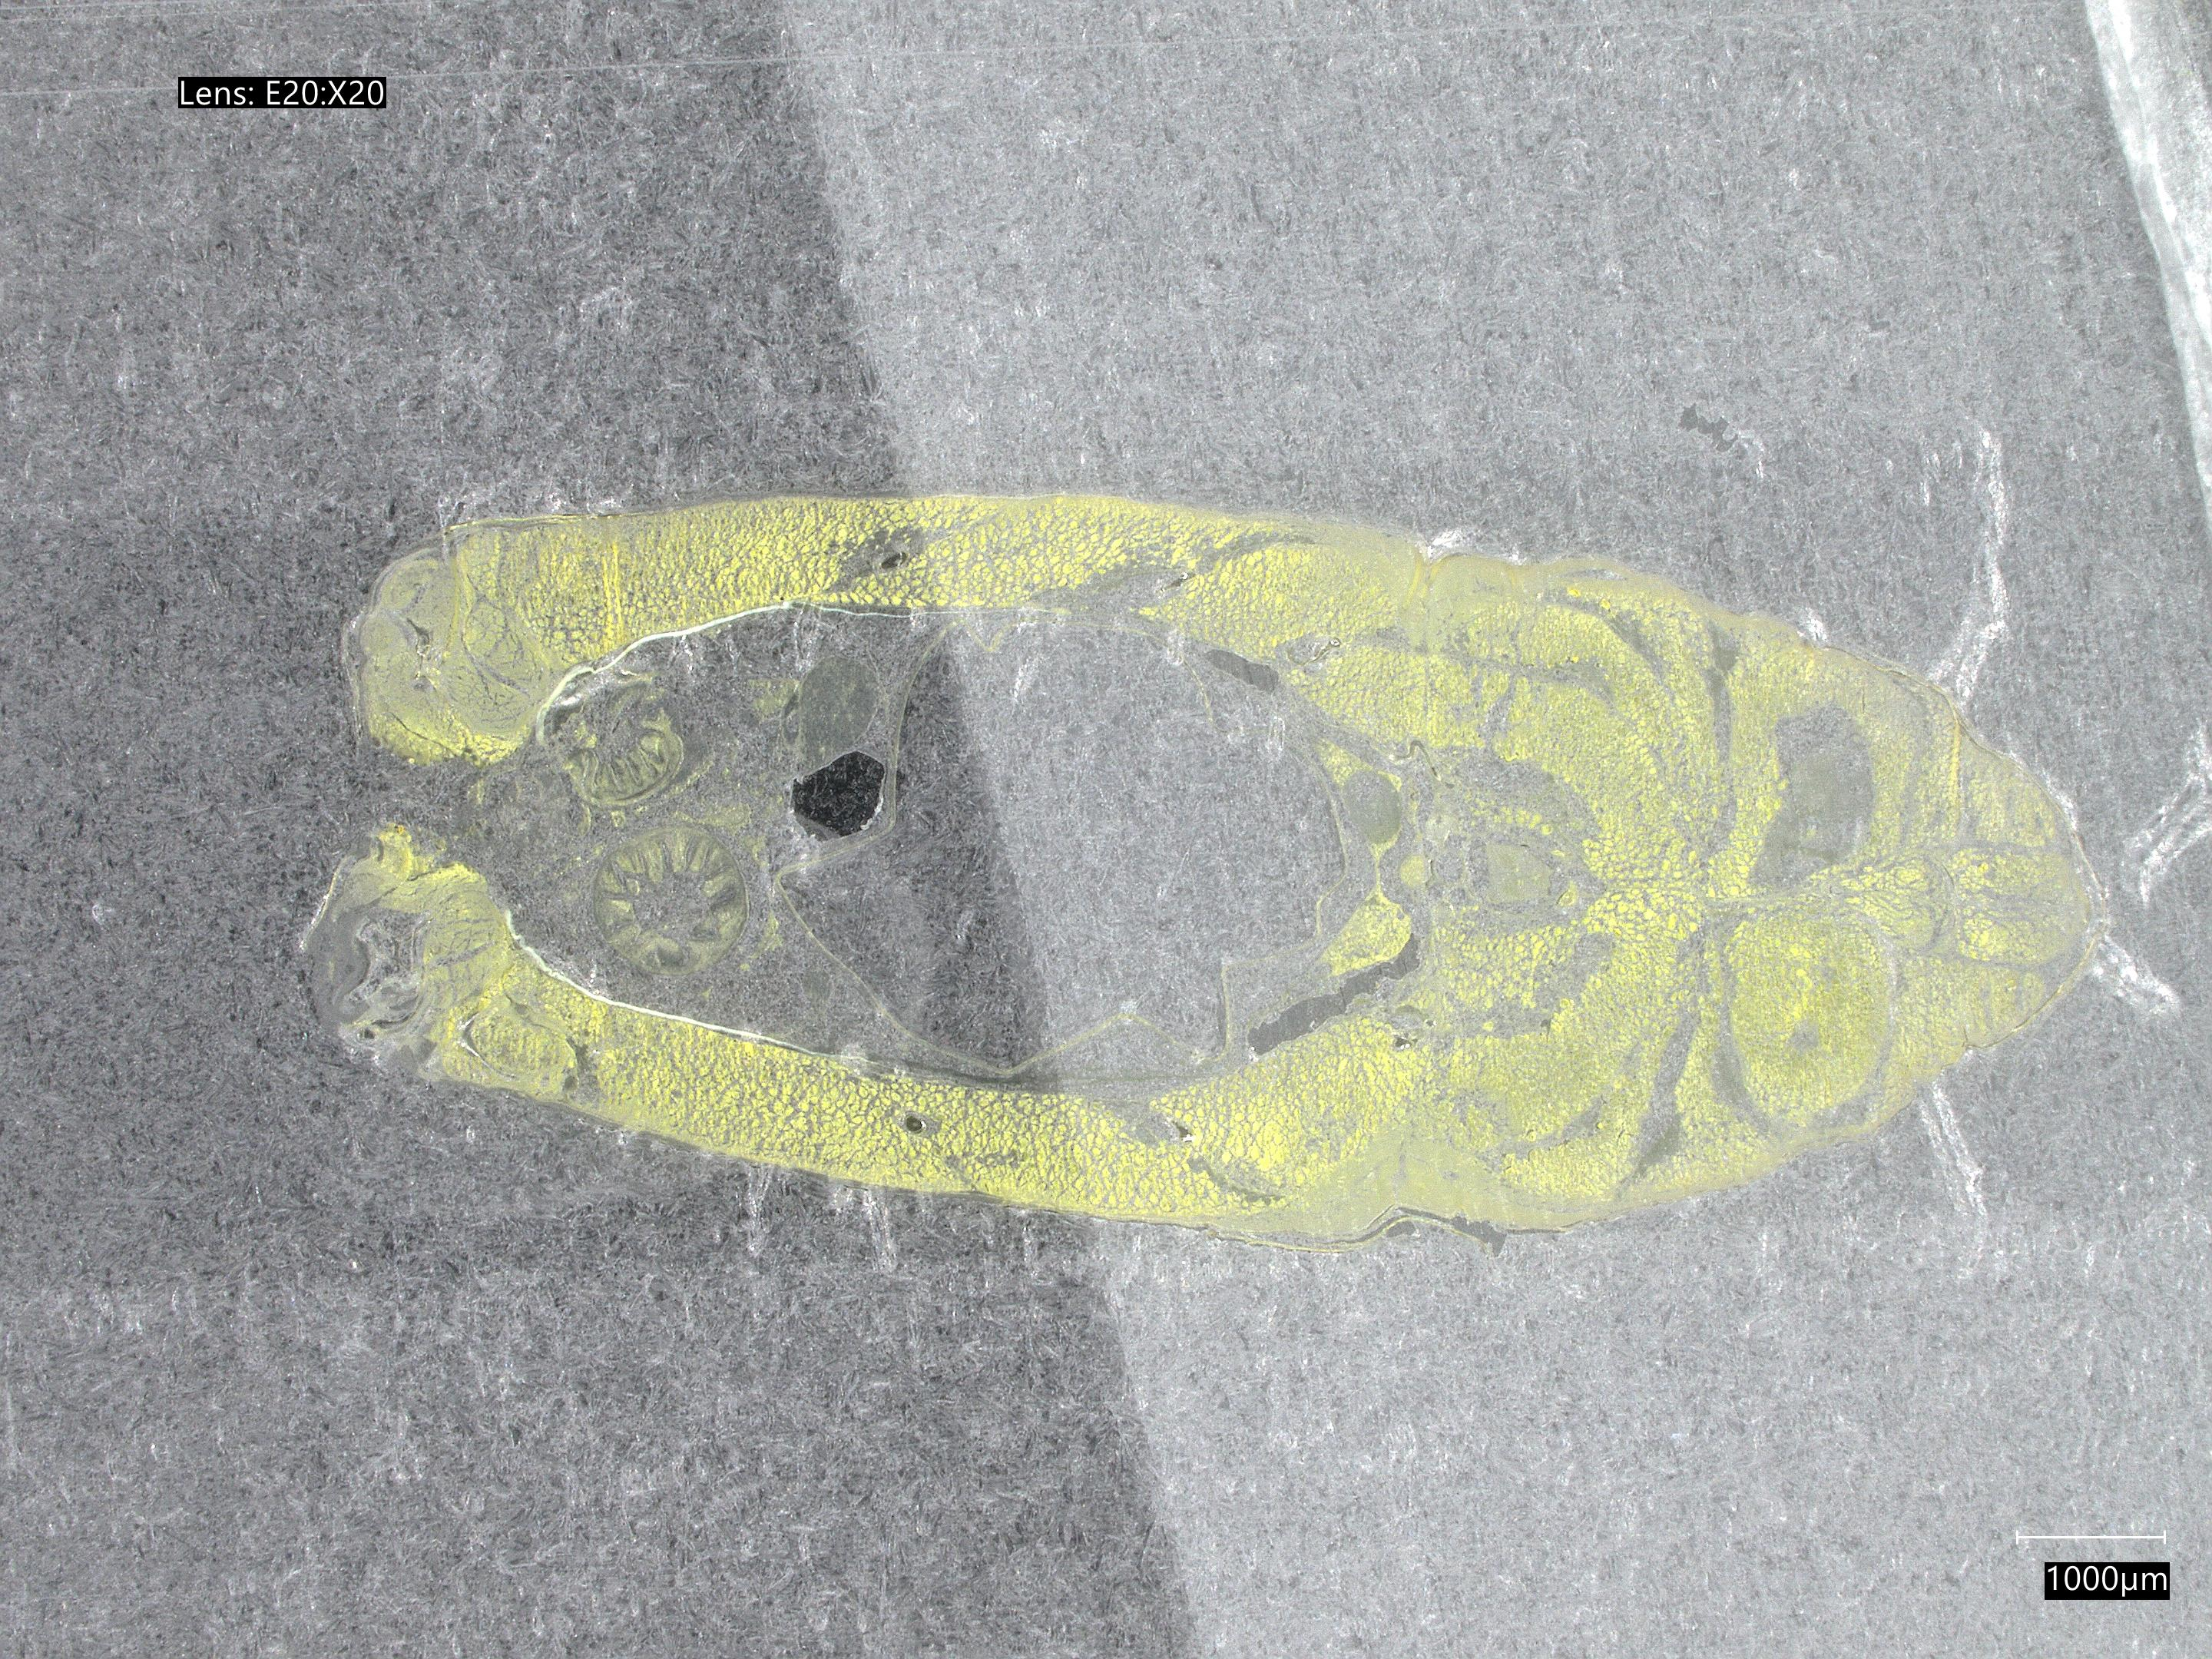
\includegraphics[width=\textwidth]{./fig/sample_1/other.jpg}
        \caption{other}
        \label{fig:other}
    \end{minipage}
    \begin{minipage}{0.32\textwidth}
        \centering
        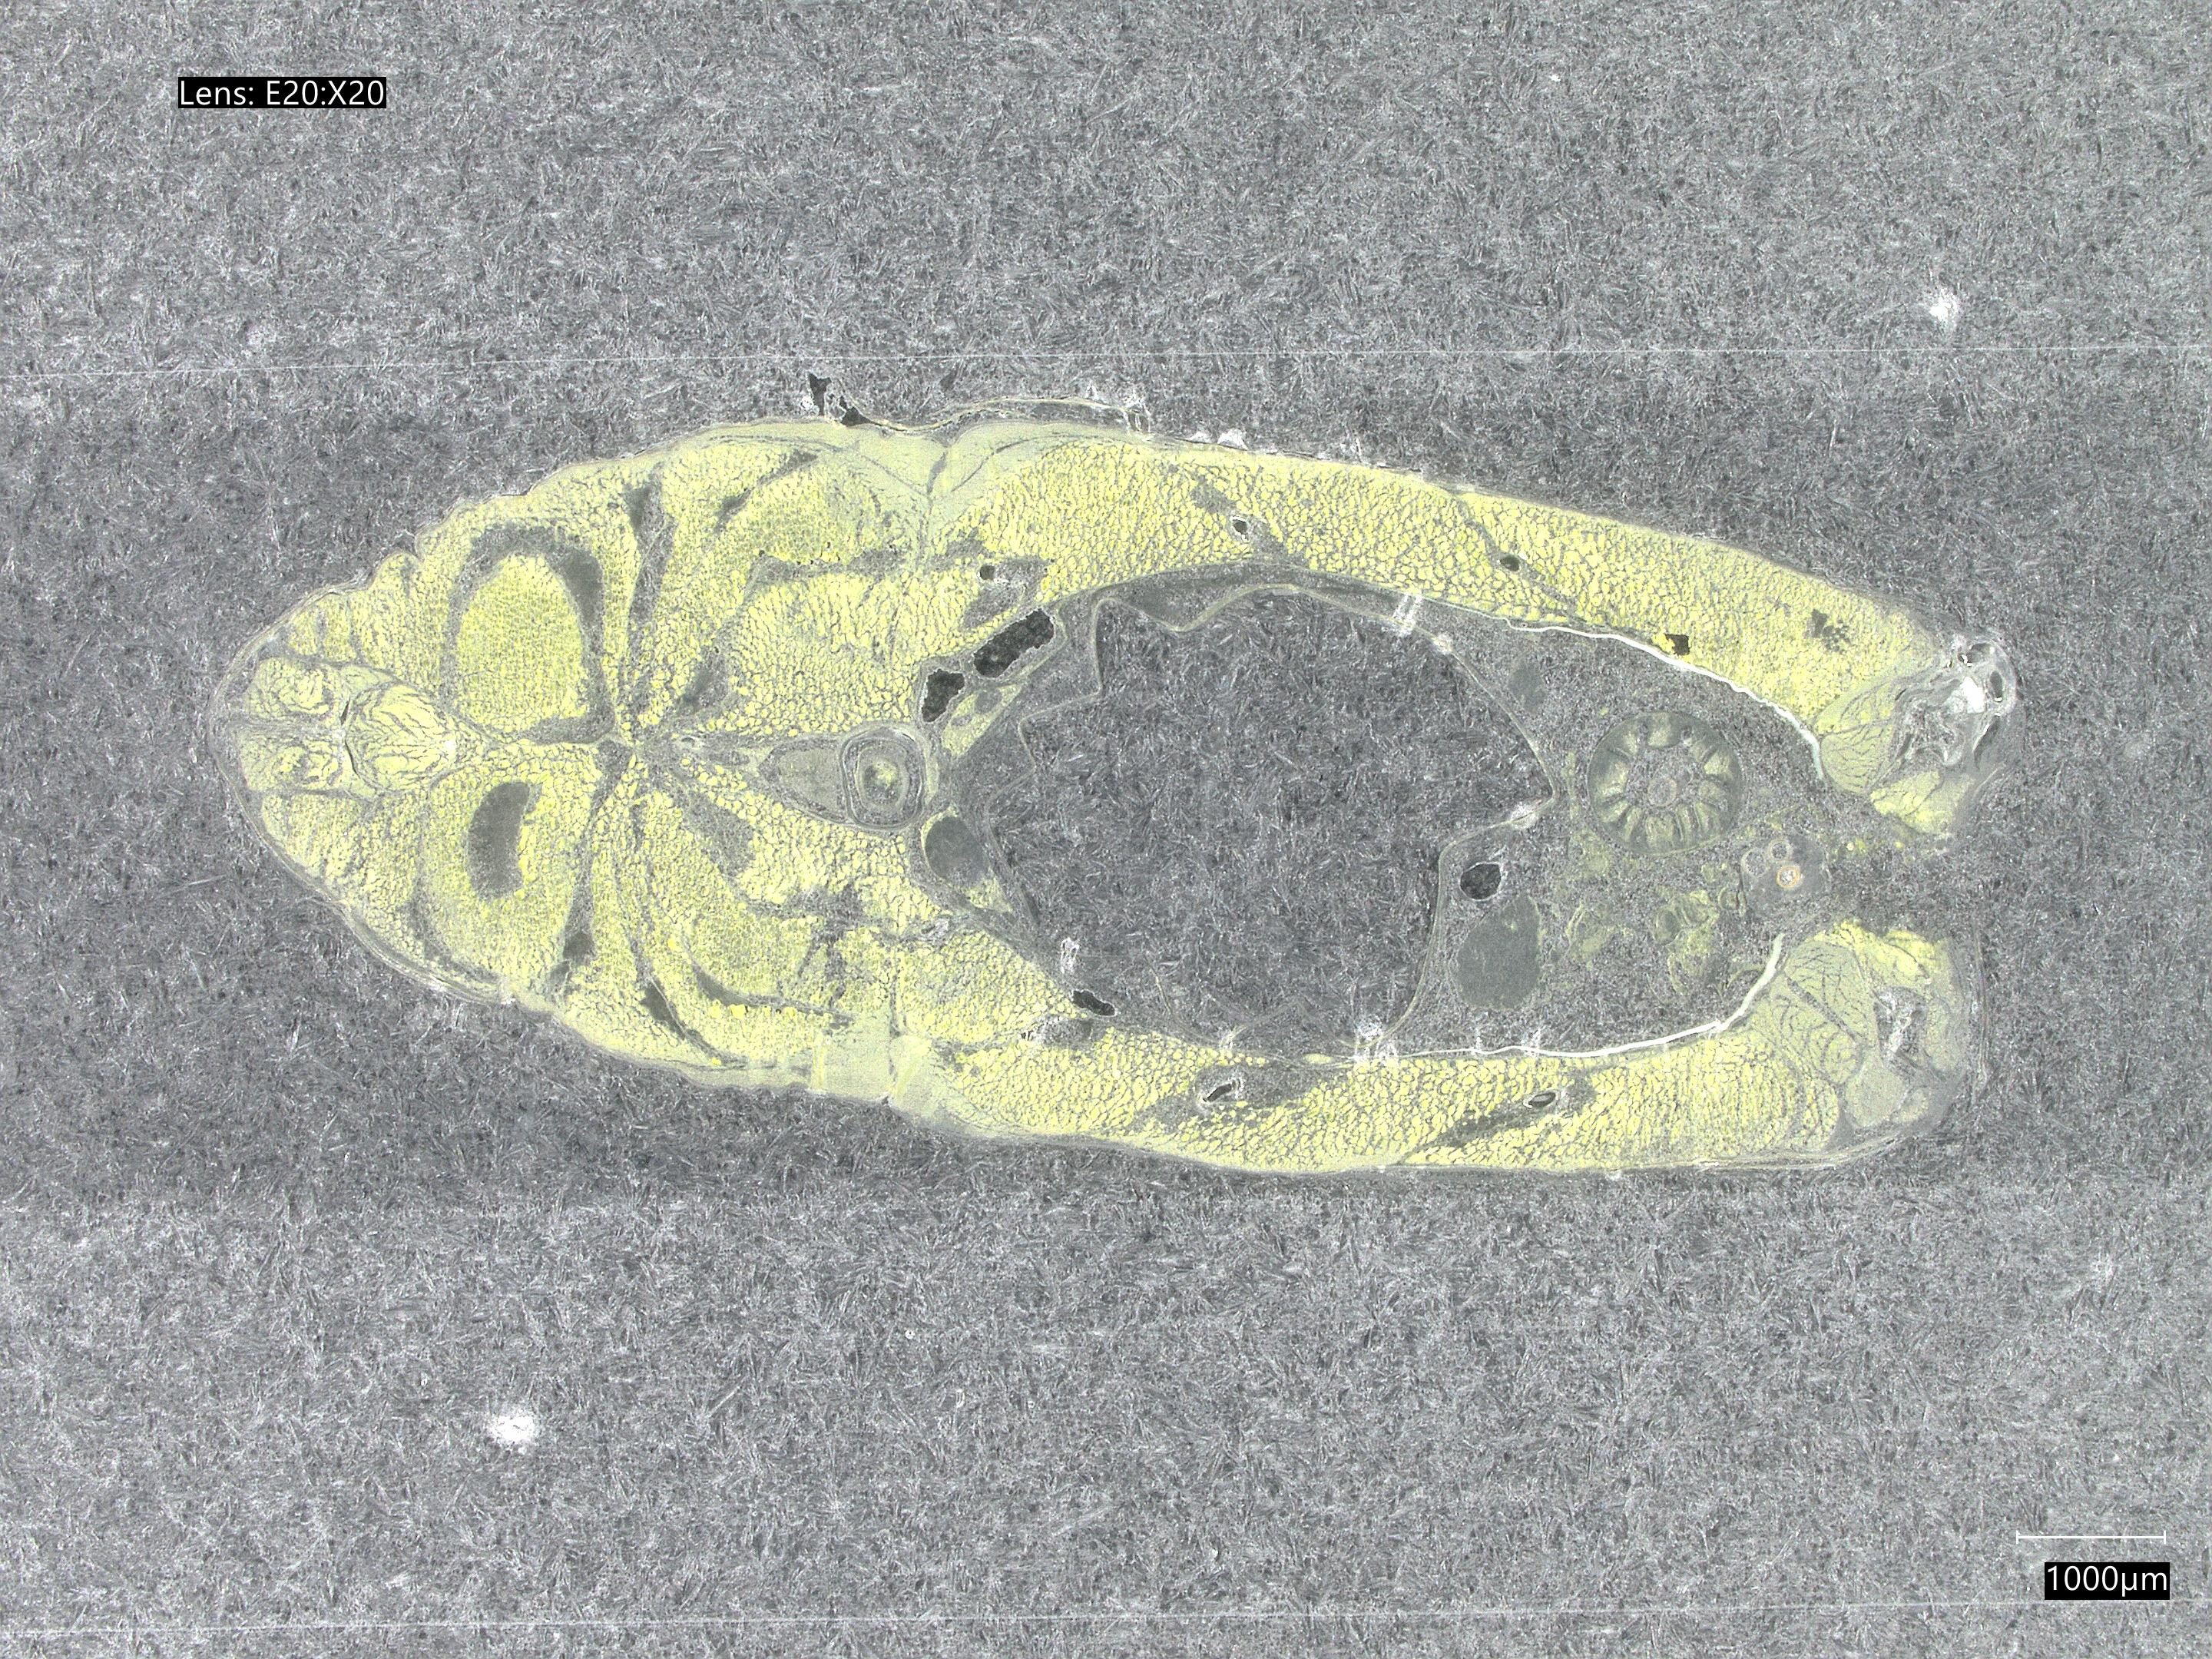
\includegraphics[width=\textwidth]{./fig/sample_1/normal.jpg}
        \caption{normal}
        \label{fig:normal}
    \end{minipage}
\end{figure}

正常的符合观察要求的切片如\autoref{fig:normal}所示。

对于每一张图片,我们需要将其标注为以上五个类别中的一个。这将作为我们的数据集,用于训练模型。

\subsection{模型1:简单CNN网络与原始图像}

对于一个新的数据集,其中模型的适当复杂度与给定图像复杂度的不确定性,首先采用基本的CNN架构来评估数据集的特性和图像的复杂性。
\begin{table}[H]
\centering
\caption{Configuration of the simple CNN model}
\begin{tabular}{ccccc}
    \toprule
    \textbf{Layer Type} & \textbf{Configuration 1a} & \textbf{Configuration 1b} & \textbf{Configuration 1c} \\
    \midrule
    Input Layer & - & - & - \\
    Conv Layer 1 & Conv3-32 (relu) & Conv3-16 (relu) & Conv3-32 (relu) \\
    Pooling Layer 1 & MaxPooling & MaxPooling& MaxPooling \\
    Conv Layer 2 & Conv3-32 (relu) & Conv3-32 (relu) & Conv3-32 (relu) \\
    Pooling Layer 2 & MaxPooling & MaxPooling& MaxPooling \\
    Conv Layer 3 & Conv3-32 (relu) & Conv3-64 (relu) & Conv3-32 (relu) \\
    Pooling Layer 3 & MaxPooling & MaxPooling& MaxPooling \\
    Flattening Layer & Flatten() & Flatten() & Flatten() \\
    FC(Full connect) & Dense(128, relu) & Dense(128, relu) & Dense(256, relu) \\
    Output Layer & - & - & - \\
    \bottomrule
\end{tabular}
\label{tab:cnn_simple_configuration}
\end{table}

简单CNN模型的配置在\autoref{tab:cnn_simple_configuration}中概述。这些初始模型,标记为配置1a、1b和1c,根据卷积层中的神经元数量和全连接层中的神经元大小进行变化。配置1a和1b根据卷积层中的神经元数量有所不同,而配置1c则在全连接层中的神经元大小上与配置1a有所不同。

预处理步骤包括将数据集分为训练集(80%)和测试集(20%)。在输入层,图像尺寸减半(从2880x2160到1440x1080),并对数据进行归一化。

在训练过程中,使用Adam优化器和交叉熵损失函数,实现早停以避免过拟合。

下面的图表显示了模型1a、1b和1c在训练周期中的准确性和损失。

\begin{figure}[H]
    \centering
    \begin{minipage}{0.49\textwidth}
        \centering
        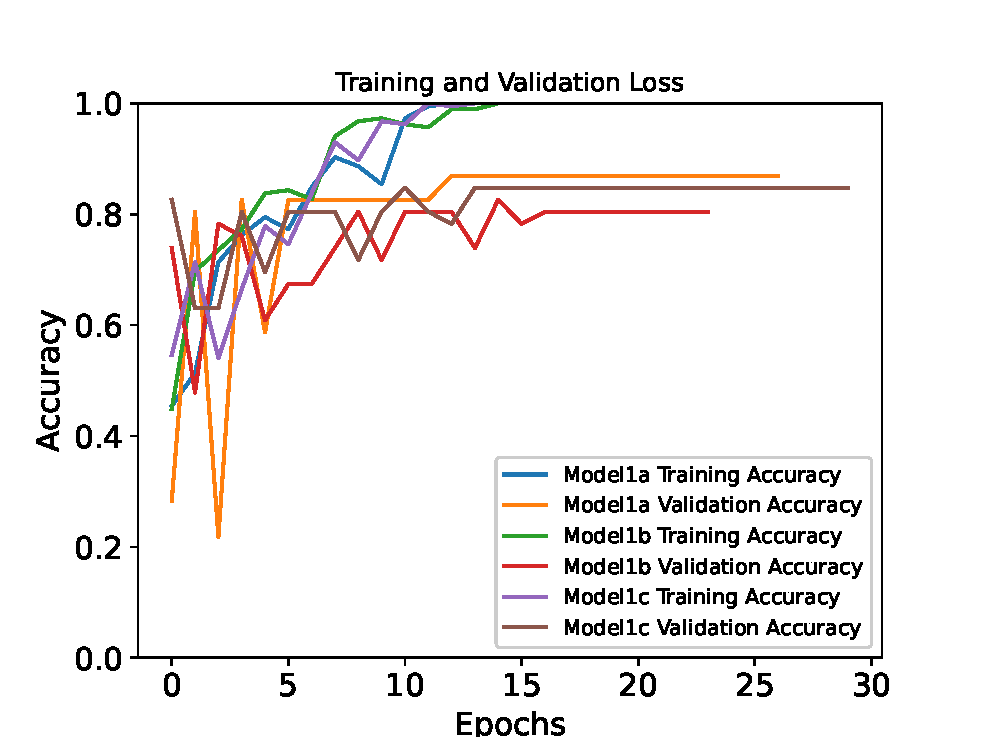
\includegraphics[width=\textwidth]{./fig/model1/accuracy11.eps}
        \caption{Model 1 accuracy}
        \label{fig:model11_acc}
    \end{minipage}
    \begin{minipage}{0.49\textwidth}
        \centering
        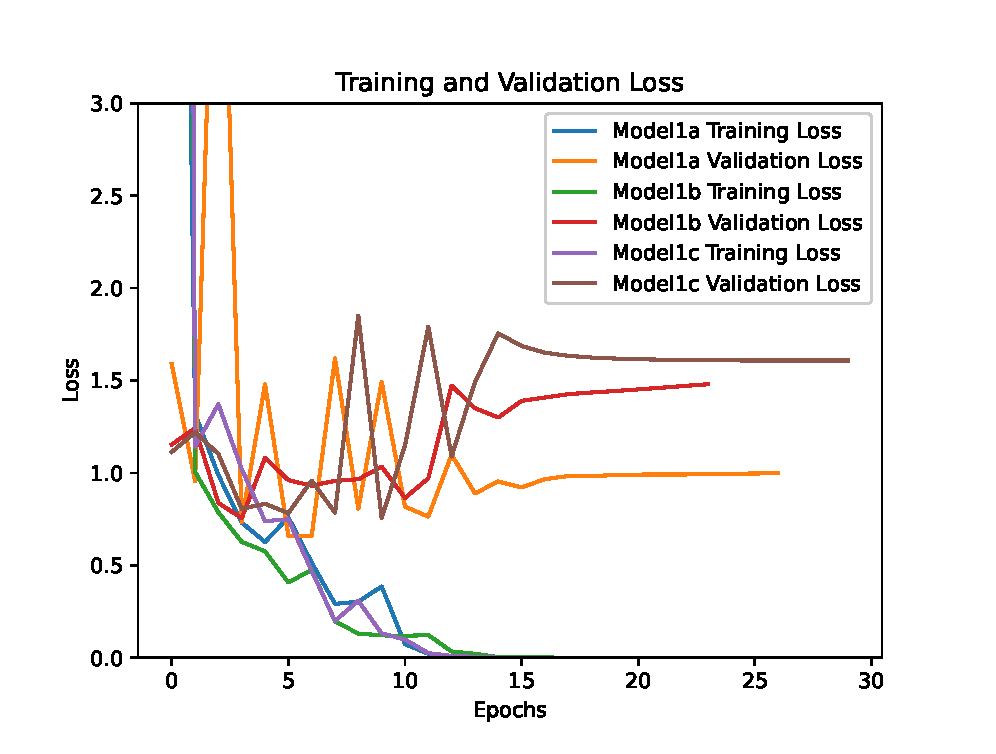
\includegraphics[width=\textwidth]{./fig/model1/loss11.eps}
        \caption{Model 1 loss}
        \label{fig:model11_loss}
    \end{minipage}
\end{figure}


从图表中可以看出,模型1a、1b和1c的训练准确性逐渐增加,随着时间的推移趋于稳定,而训练损失则逐渐减少,接近零。这表明模型从训练数据中学习得相对良好。然而,对于验证集,所有三个模型的准确性在80%到85%的范围内稳定,而在某些情况下,验证损失相对较高,特别是在模型1a中,它接近2.5并显示出显著的波动。这表明存在一定程度的过拟合,即模型在训练数据上的表现优于在未见过的数据上。值得注意的是,模型1c在验证损失方面表现最好,表明其结构或参数调整可能更有效地提高泛化能力。

这里过拟合的可能原因是模型的复杂度相对于数据集的复杂度不足,表明模型可能没有有效地从数据中提取特征。尽管模型在训练集上达到了高准确性和低损失,但它们在验证集上的泛化能力需要增强。

为了提高模型的准确性,考虑对图像进行预处理并手动帮助模型进行特征提取可能是有益的,这有助于模型更好地泛化到新数据。

\subsection{图像预处理改进}

在模型性能不佳的情况下,可能是由于图像的复杂性阻碍了模型有效提取重要特征。因此,考虑使用边缘检测和阈值分割等图像预处理技术,以突出模型识别的所需特征,并减少无关特征和噪声,从而提高后续深度学习模型的准确性。

\subsubsection{边缘检测}

如3.2.1节所述,边缘检测的原理涉及识别像素强度(梯度)的变化,以确定图像内的边缘。

在进行边缘检测之前,首先应用一个初始预处理步骤——高斯模糊。高斯模糊的理由是它有助于减少图像中的噪声,平滑梯度过渡,并降低检测到假边缘的可能性,从而提高边缘检测的准确性\cite{4.3}。我们试验了21、41、61和81大小的高斯核,分别对应于图像宽度的1%、2%、3%和4%。

下面显示了高斯模糊后的图像。为了更好地演示高斯核大小对边缘检测的影响,模糊后使用Sobel算子计算边缘并增加50个单位的亮度以提高可见性。

\begin{figure}
    \centering
    \begin{minipage}{0.24\textwidth}
        \centering
        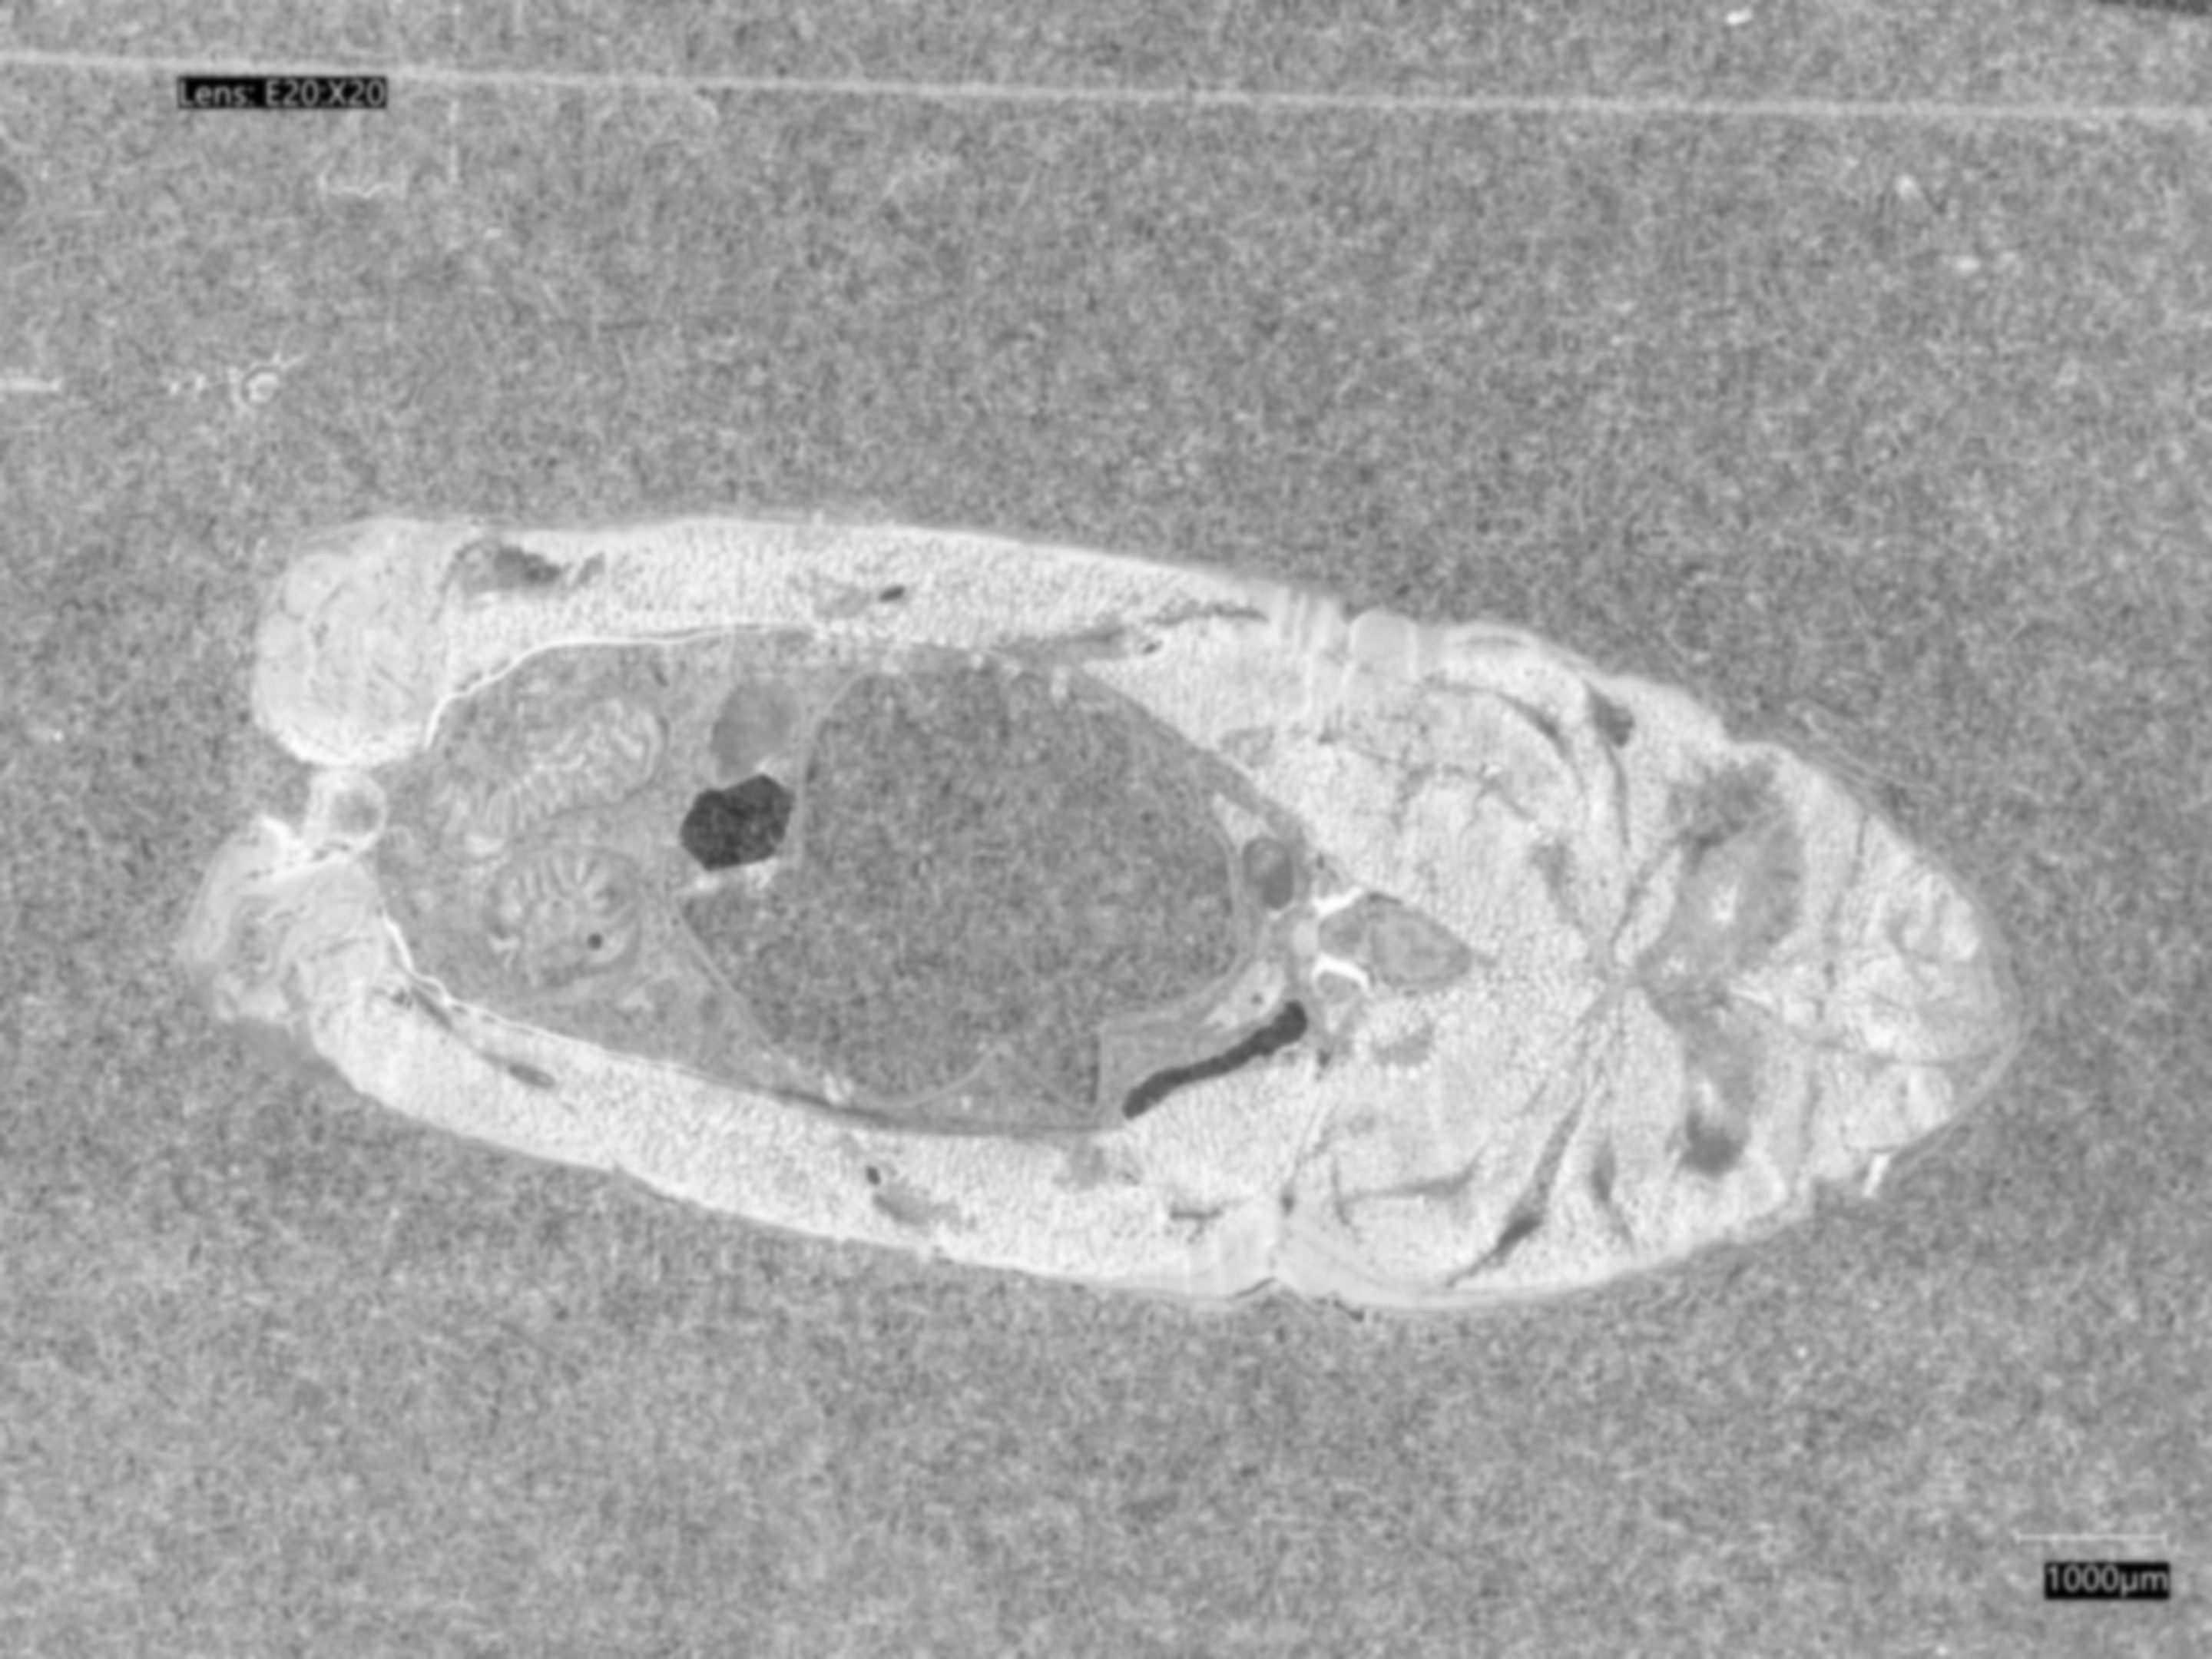
\includegraphics[width=\textwidth]{./fig/gausssian/blurred21.jpg}
        \caption*{k=21}
        \label{fig:blurred21}
    \end{minipage}
    \begin{minipage}{0.24\textwidth}
        \centering
        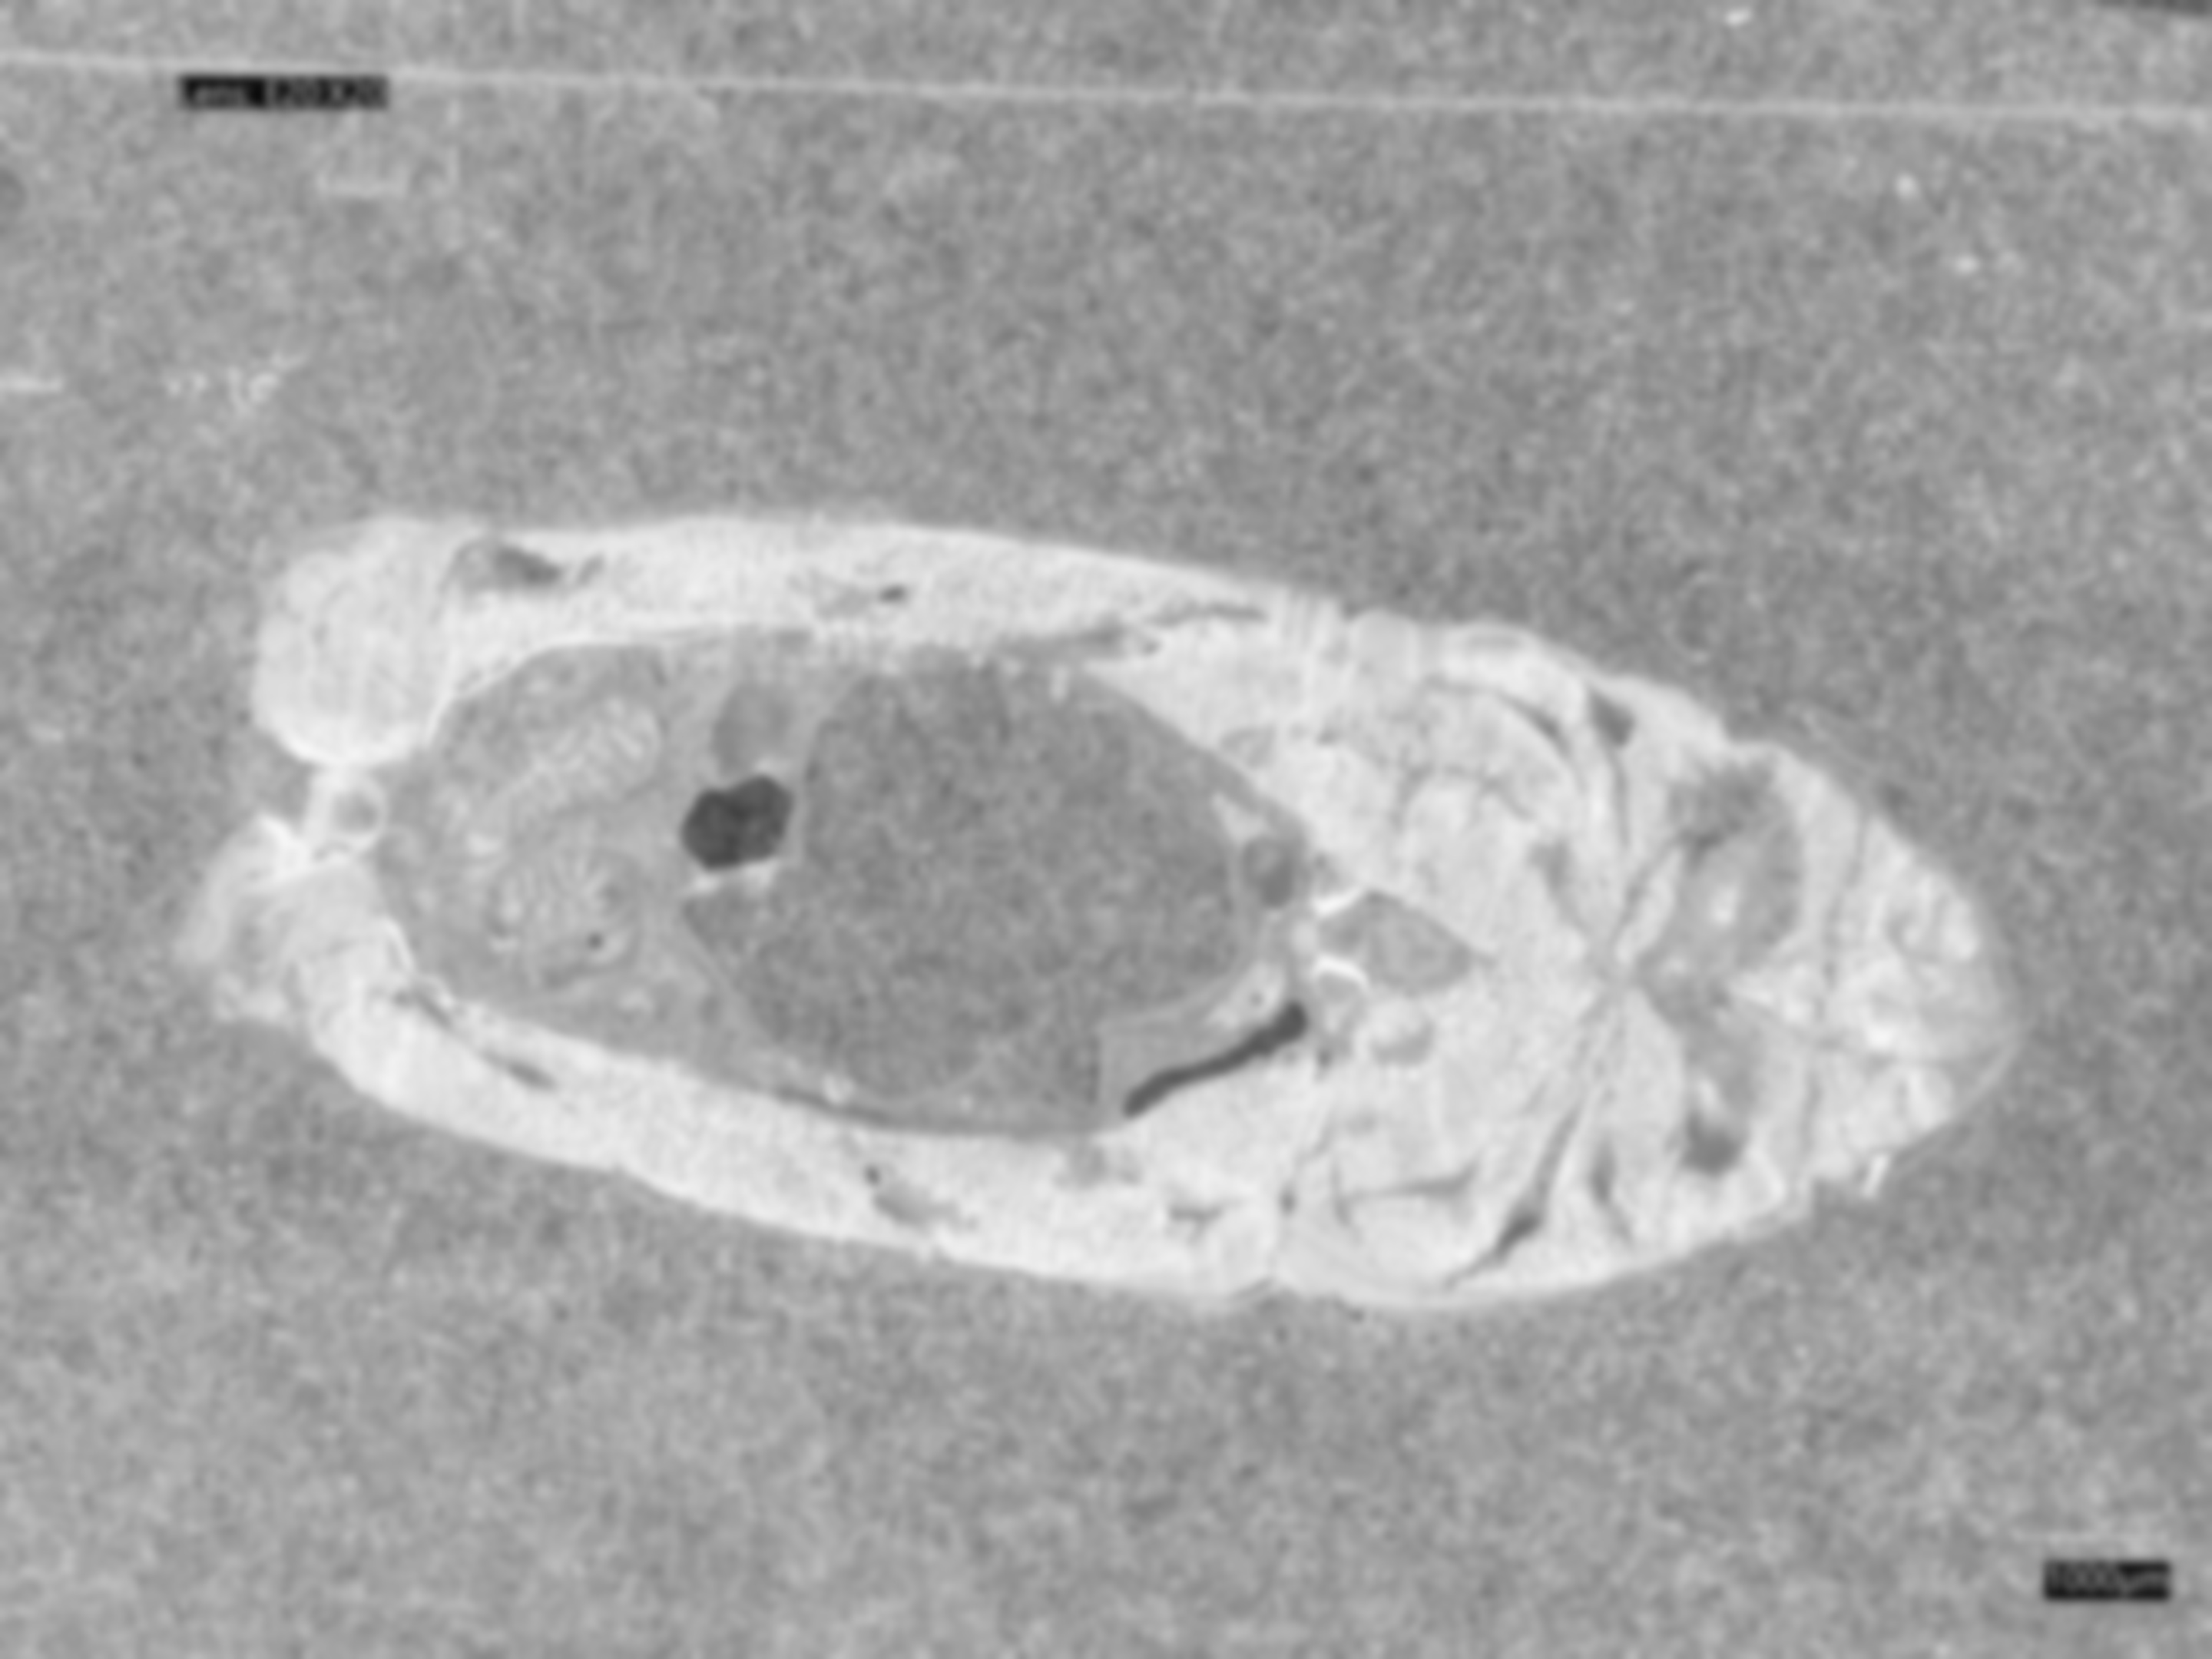
\includegraphics[width=\textwidth]{./fig/gausssian/blurred41.jpg}
        \caption*{k=41}
        \label{fig:blurred41}
    \end{minipage}
    \begin{minipage}{0.24\textwidth}
        \centering
        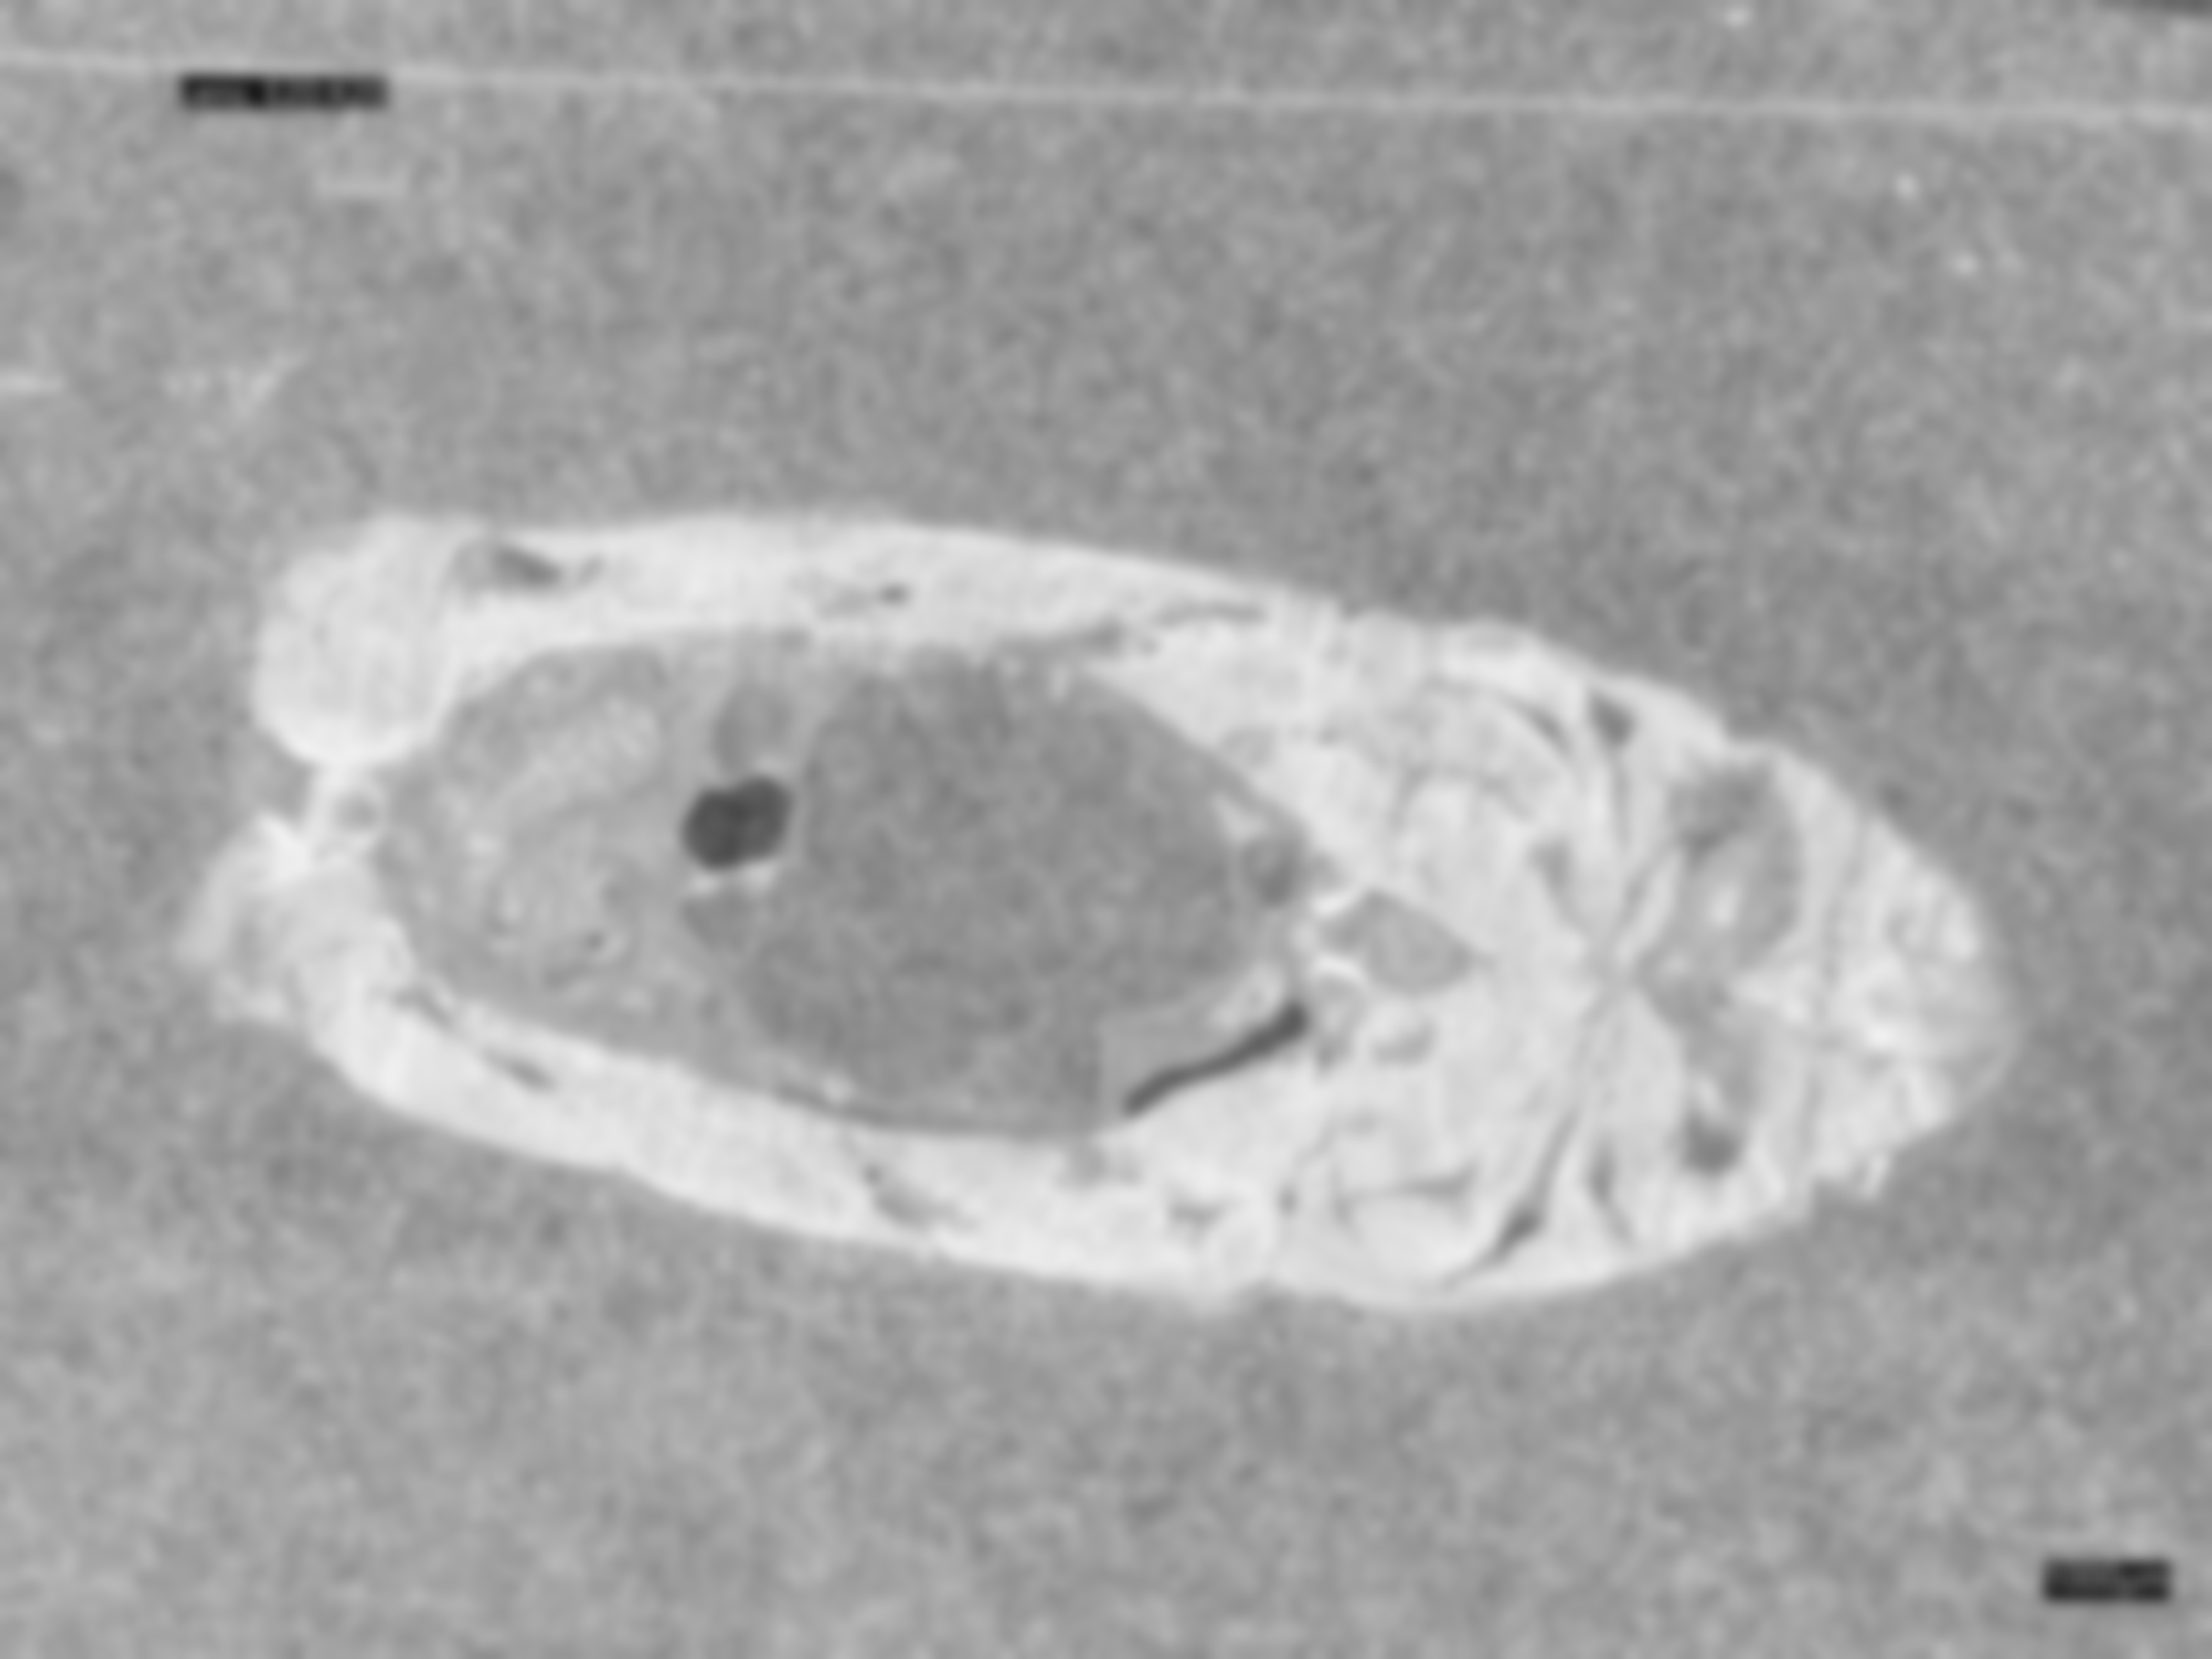
\includegraphics[width=\textwidth]{./fig/gausssian/blurred61.jpg}
        \caption*{k=61}
        \label{fig:blurred61}
    \end{minipage}
    \begin{minipage}{0.24\textwidth}
        \centering
        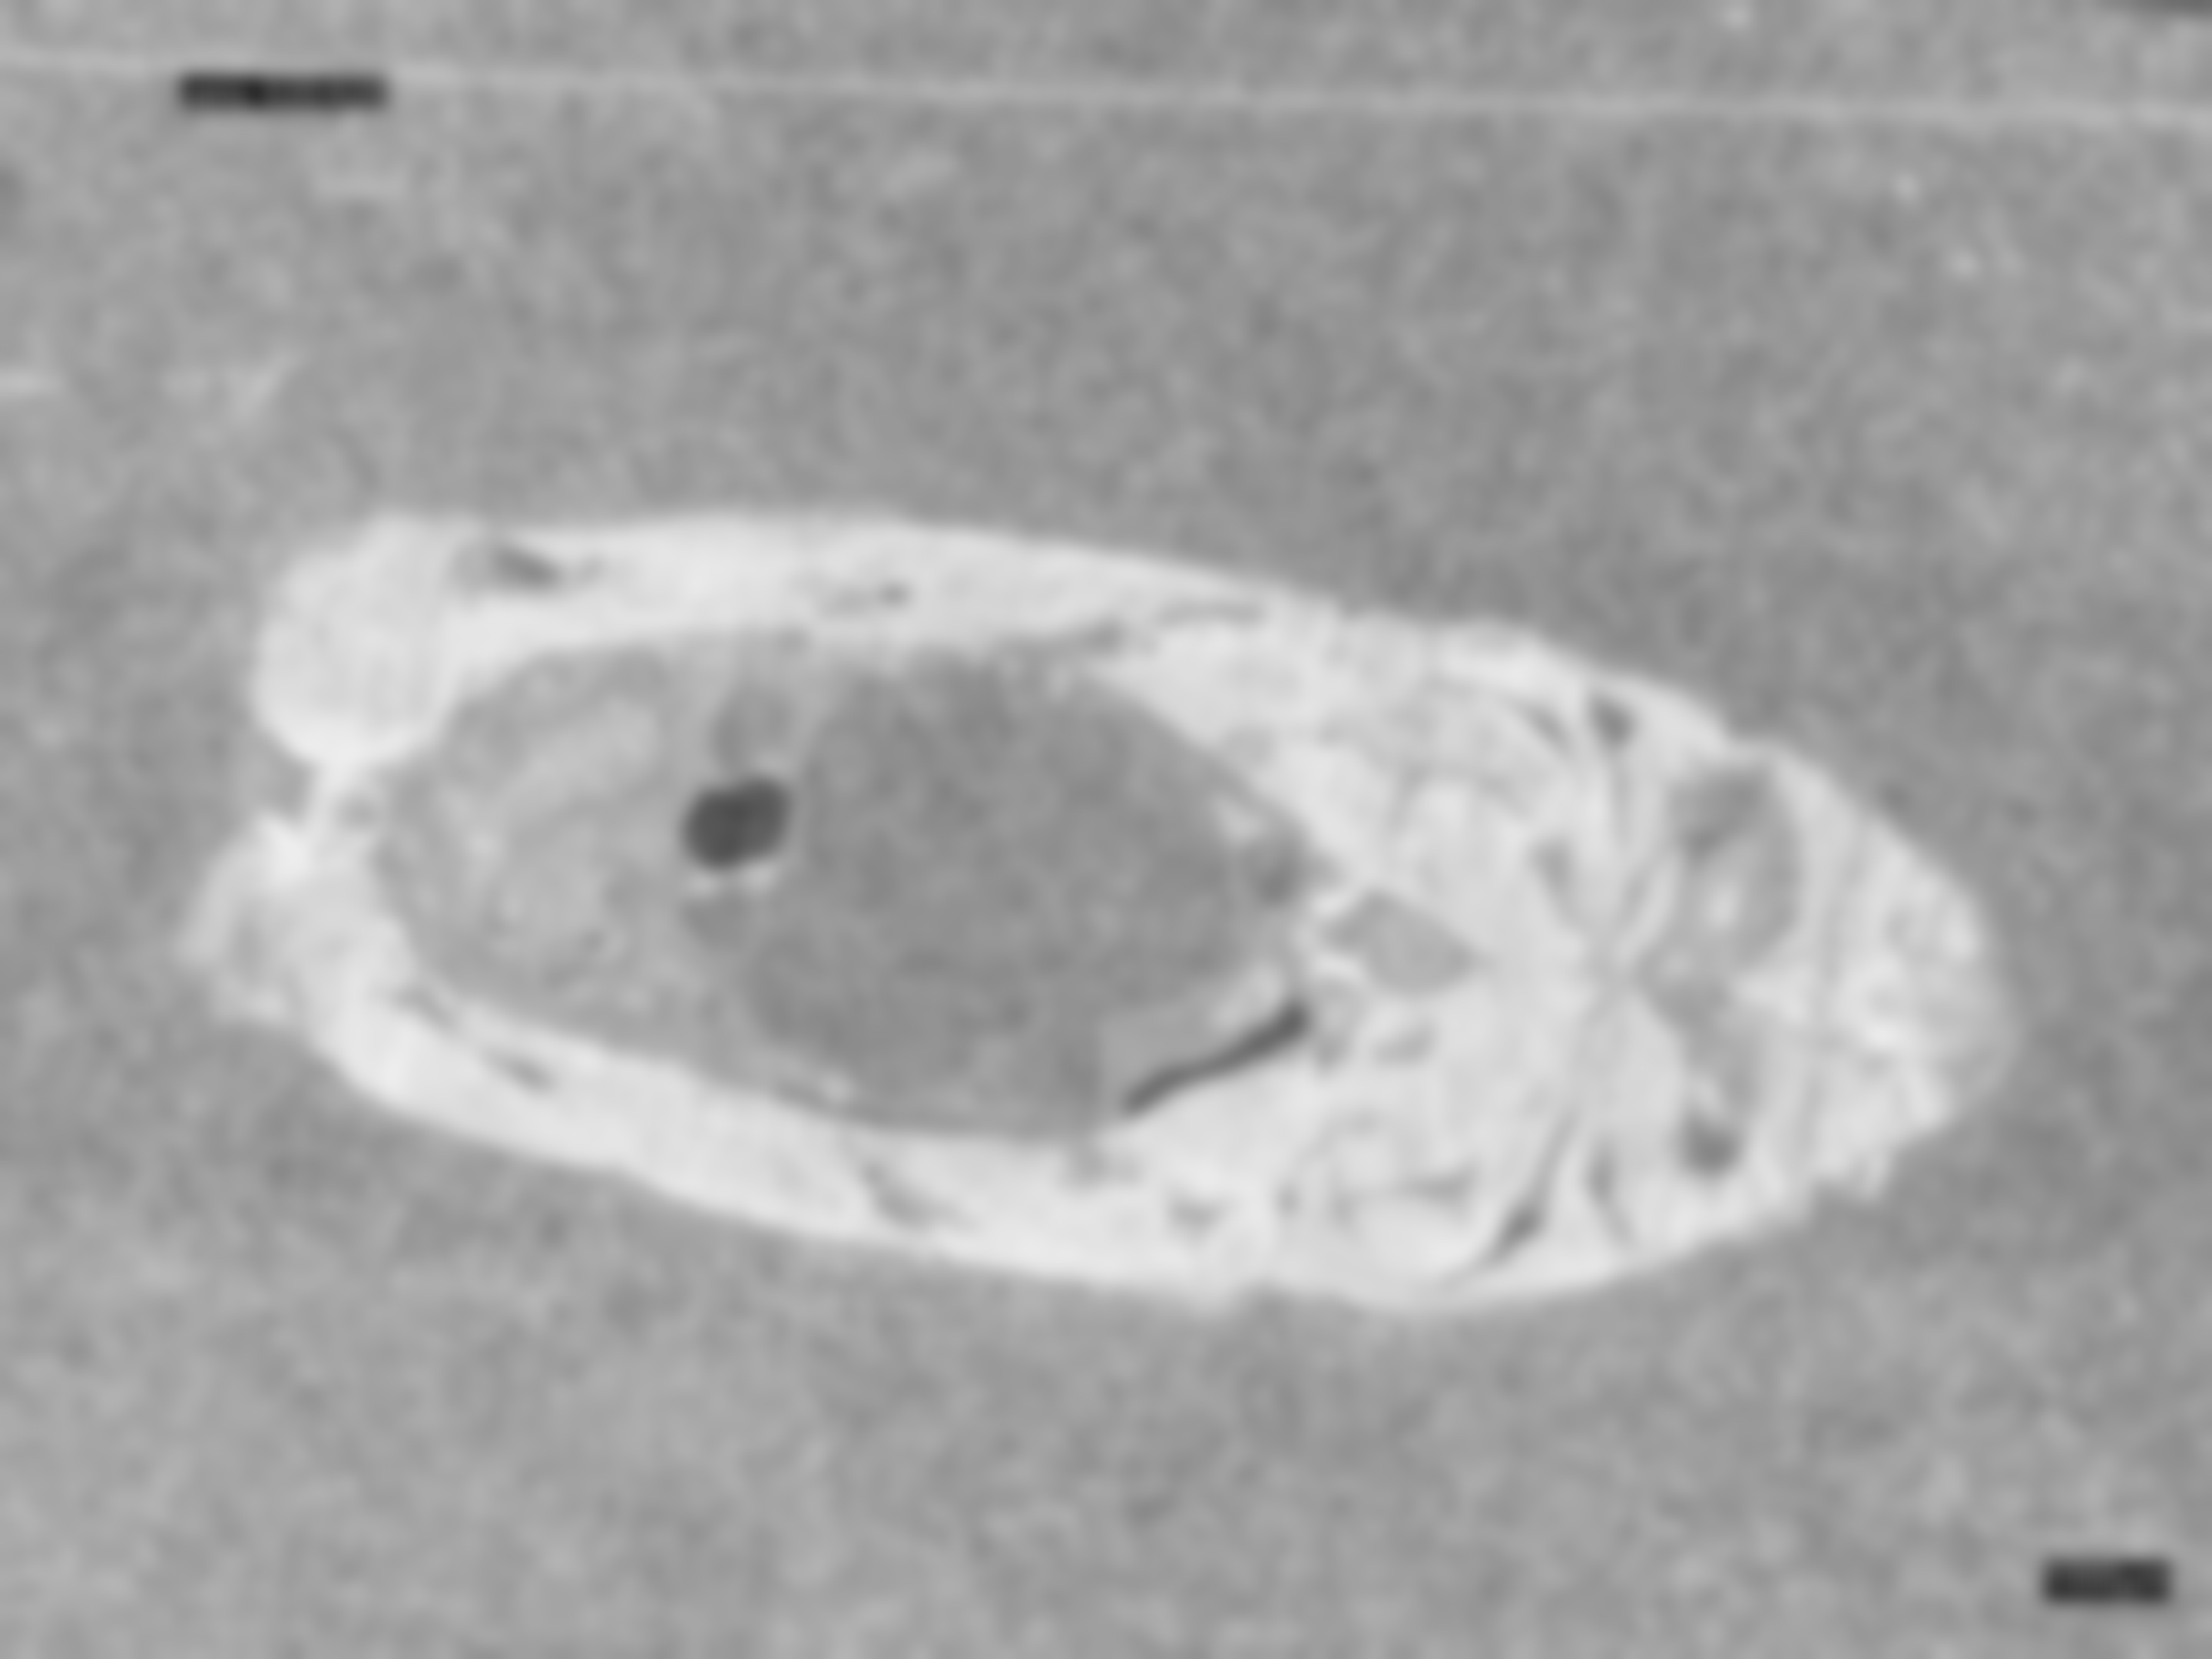
\includegraphics[width=\textwidth]{./fig/gausssian/blurred81.jpg}
        \caption*{k=81}
        \label{fig:blurred81}
    \end{minipage}
    \caption{Images post-Gaussian blur}
    \label{fig:blurred}
\end{figure}

\begin{figure}
    \centering
    \begin{minipage}{0.24\textwidth}
        \centering
        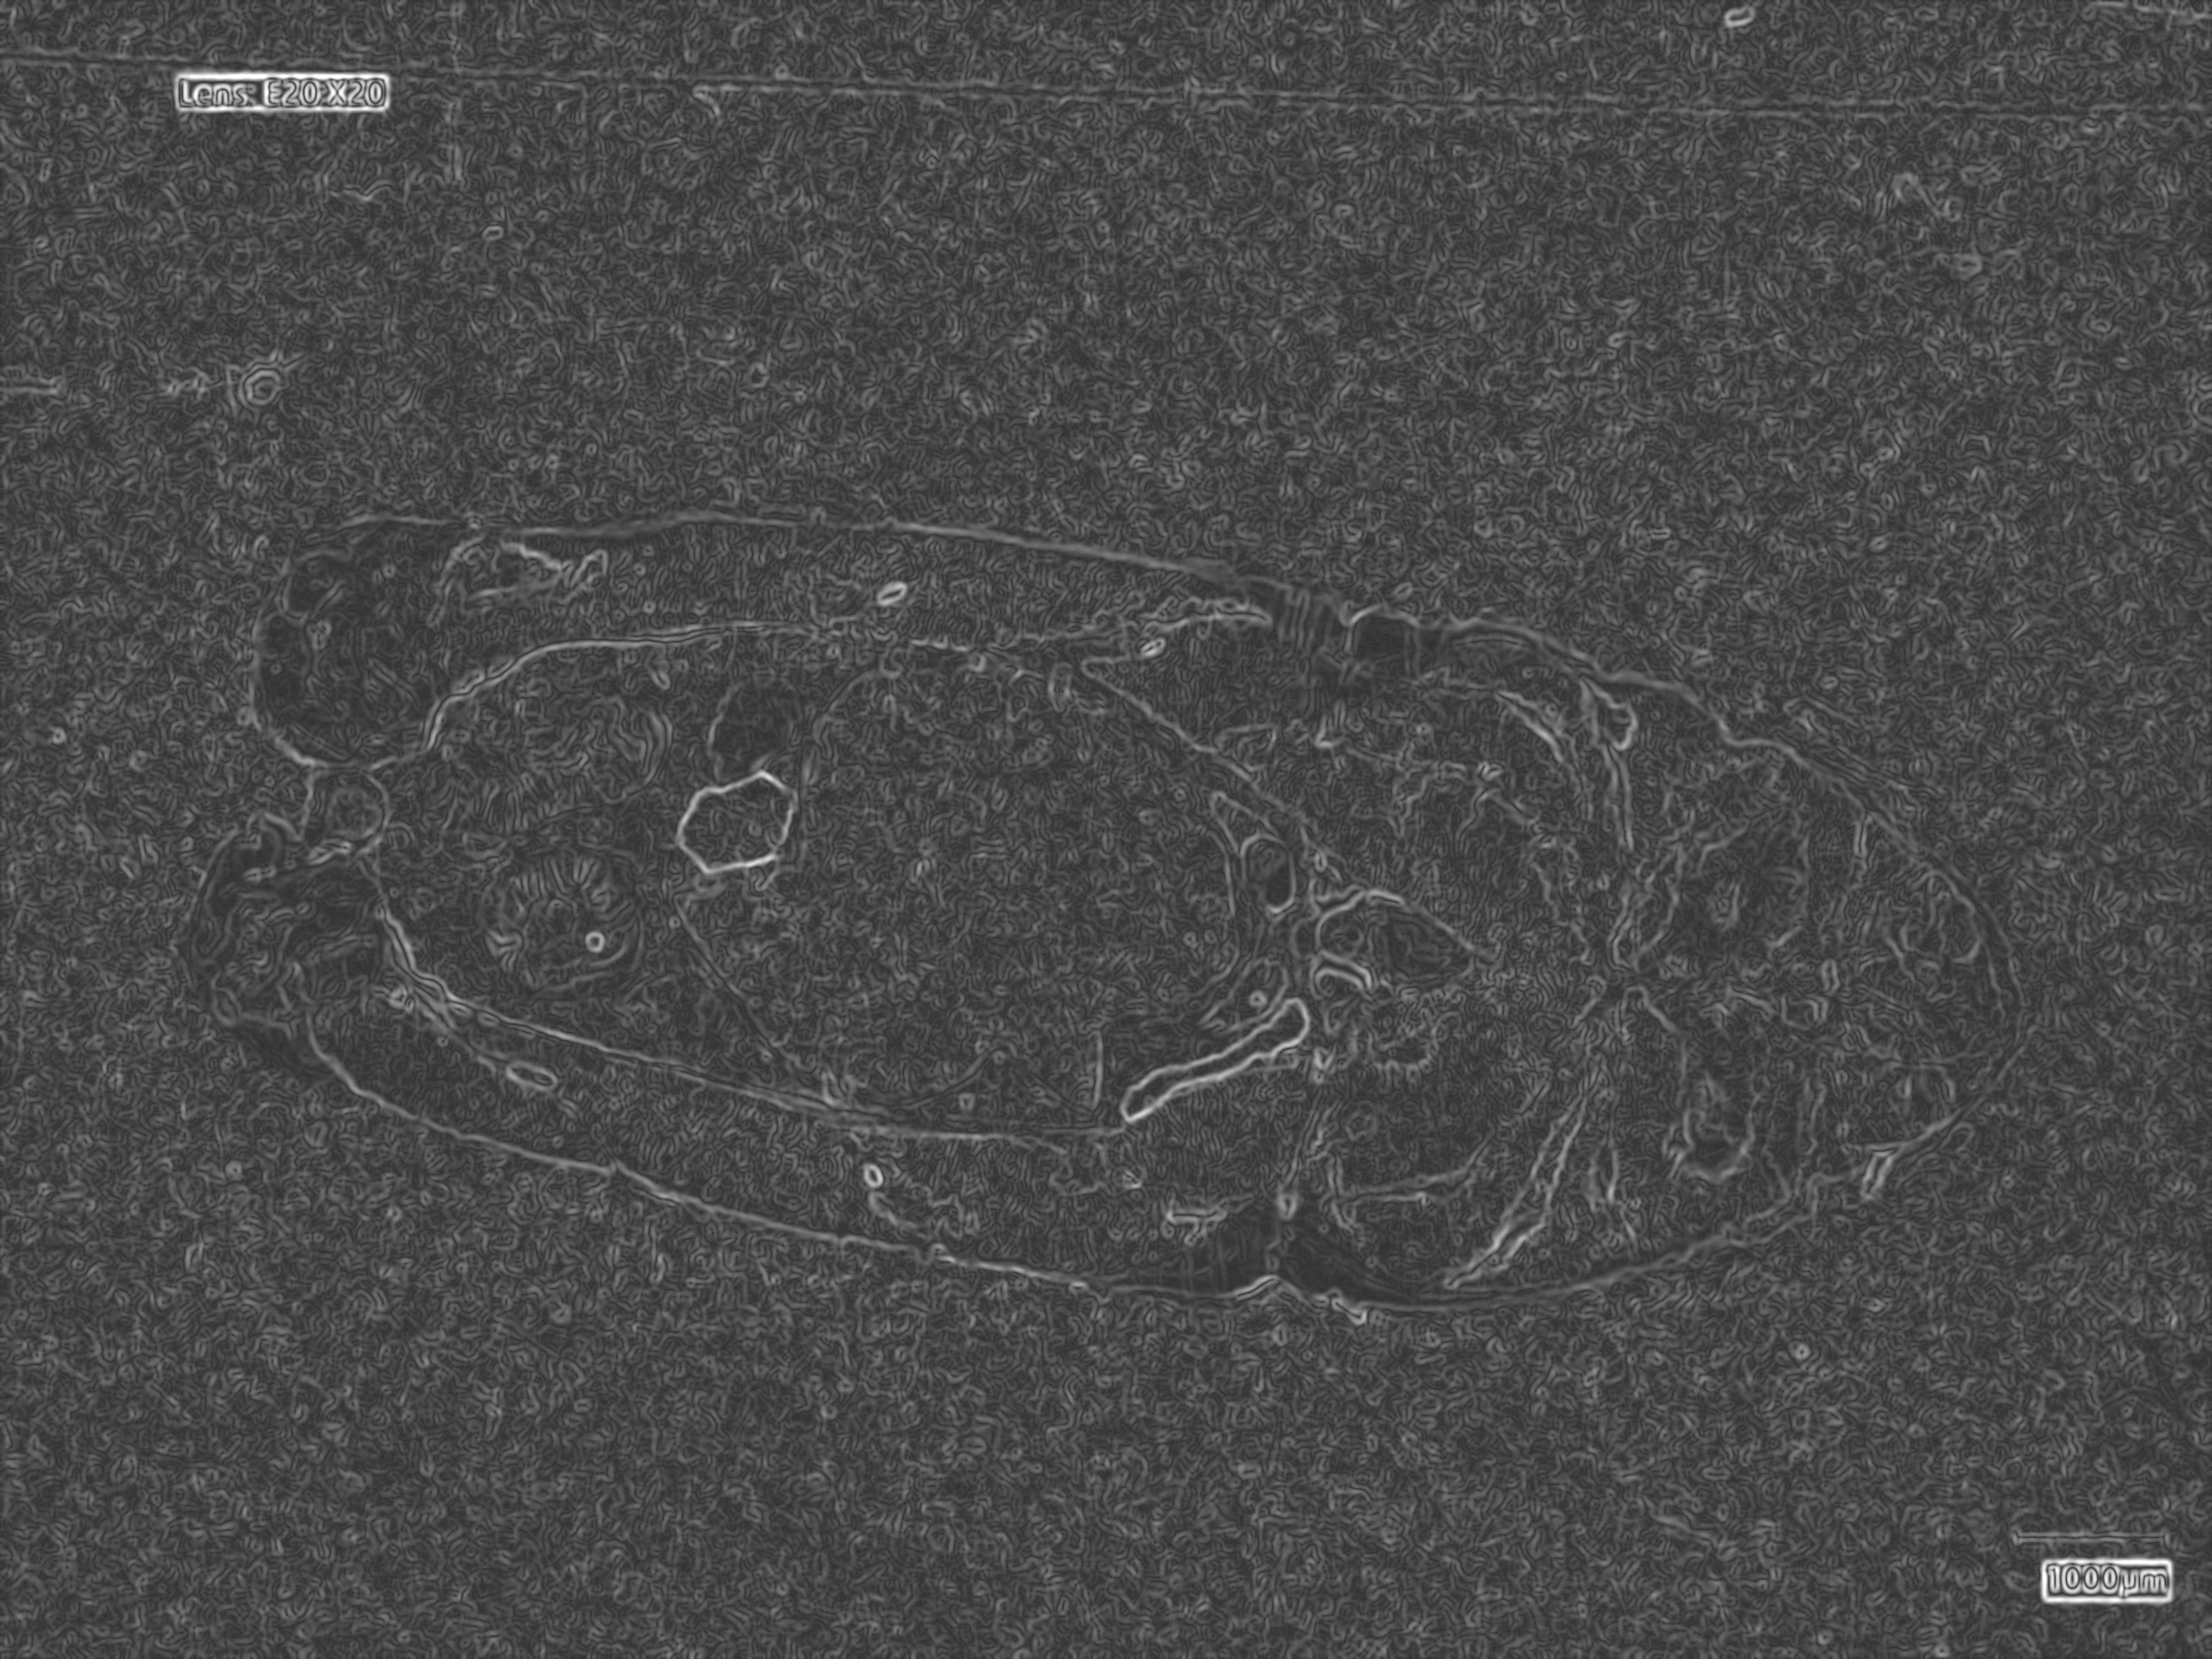
\includegraphics[width=\textwidth]{./fig/gausssian/sobel21.jpg}
        \caption*{k=21}
        \label{fig:sobel21}
    \end{minipage}
    \begin{minipage}{0.24\textwidth}
        \centering
        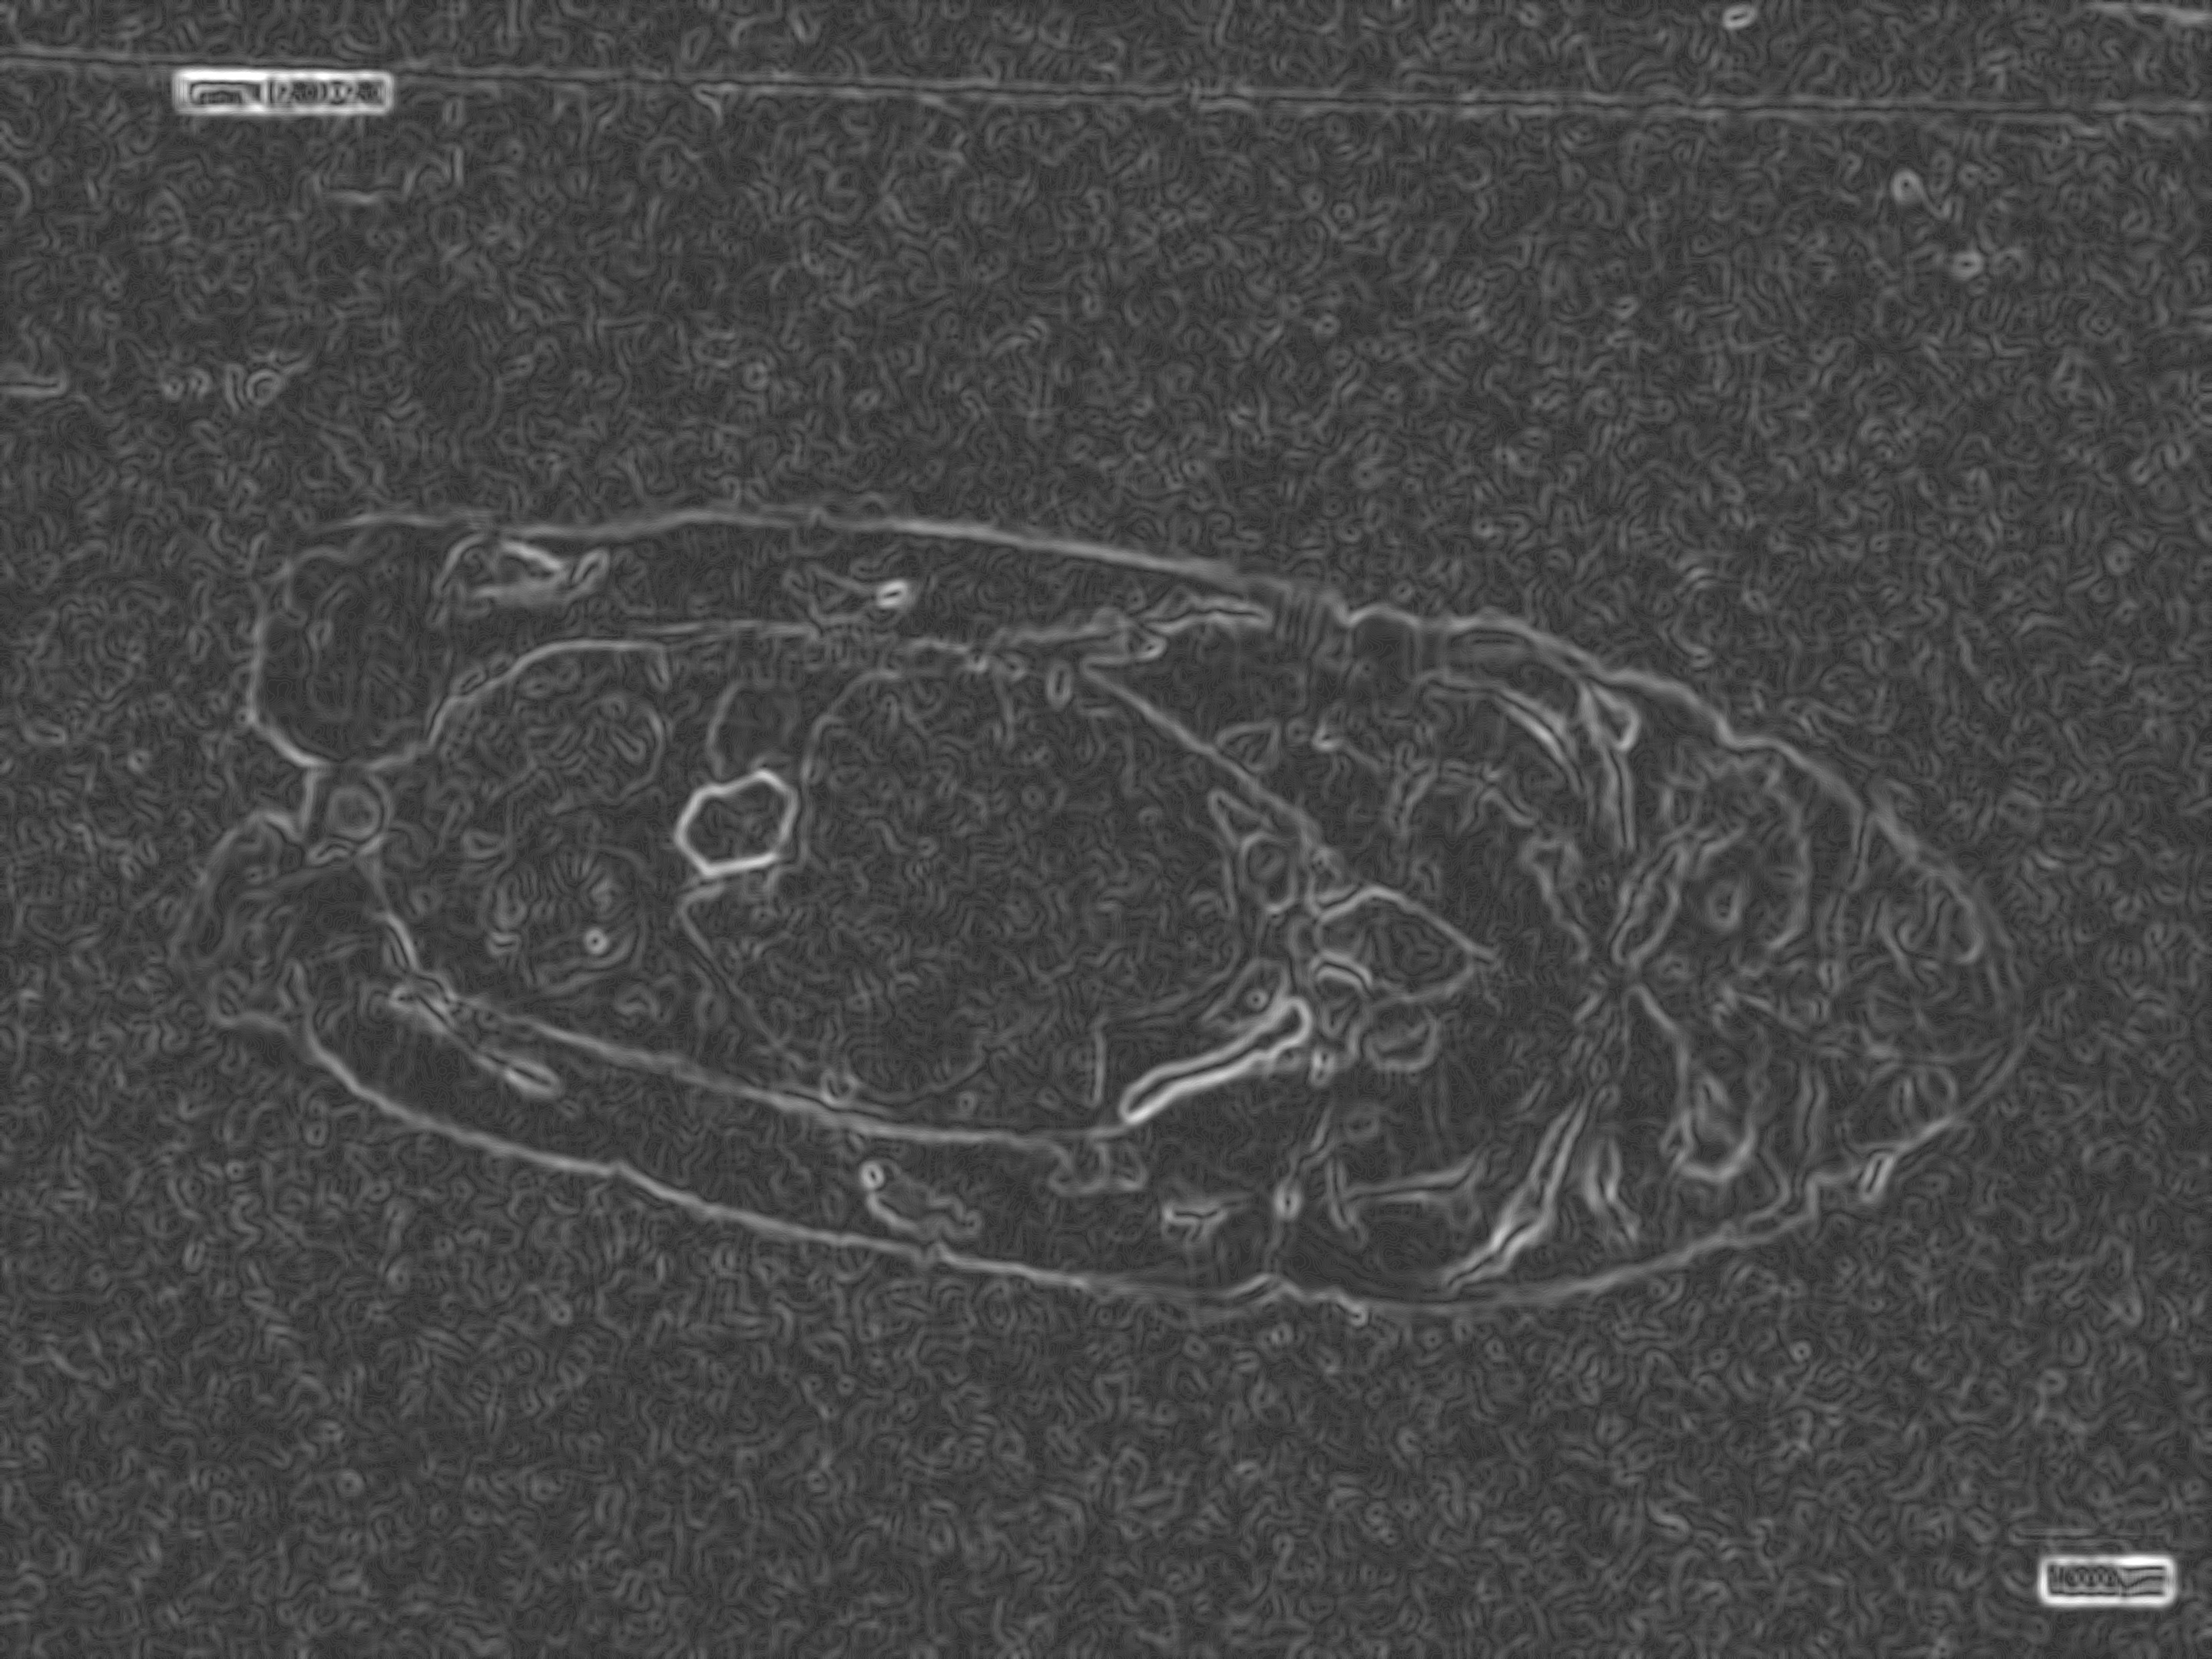
\includegraphics[width=\textwidth]{./fig/gausssian/sobel41.jpg}
        \caption*{k=41}
        \label{fig:sobel41}
    \end{minipage}
    \begin{minipage}{0.24\textwidth}
        \centering
        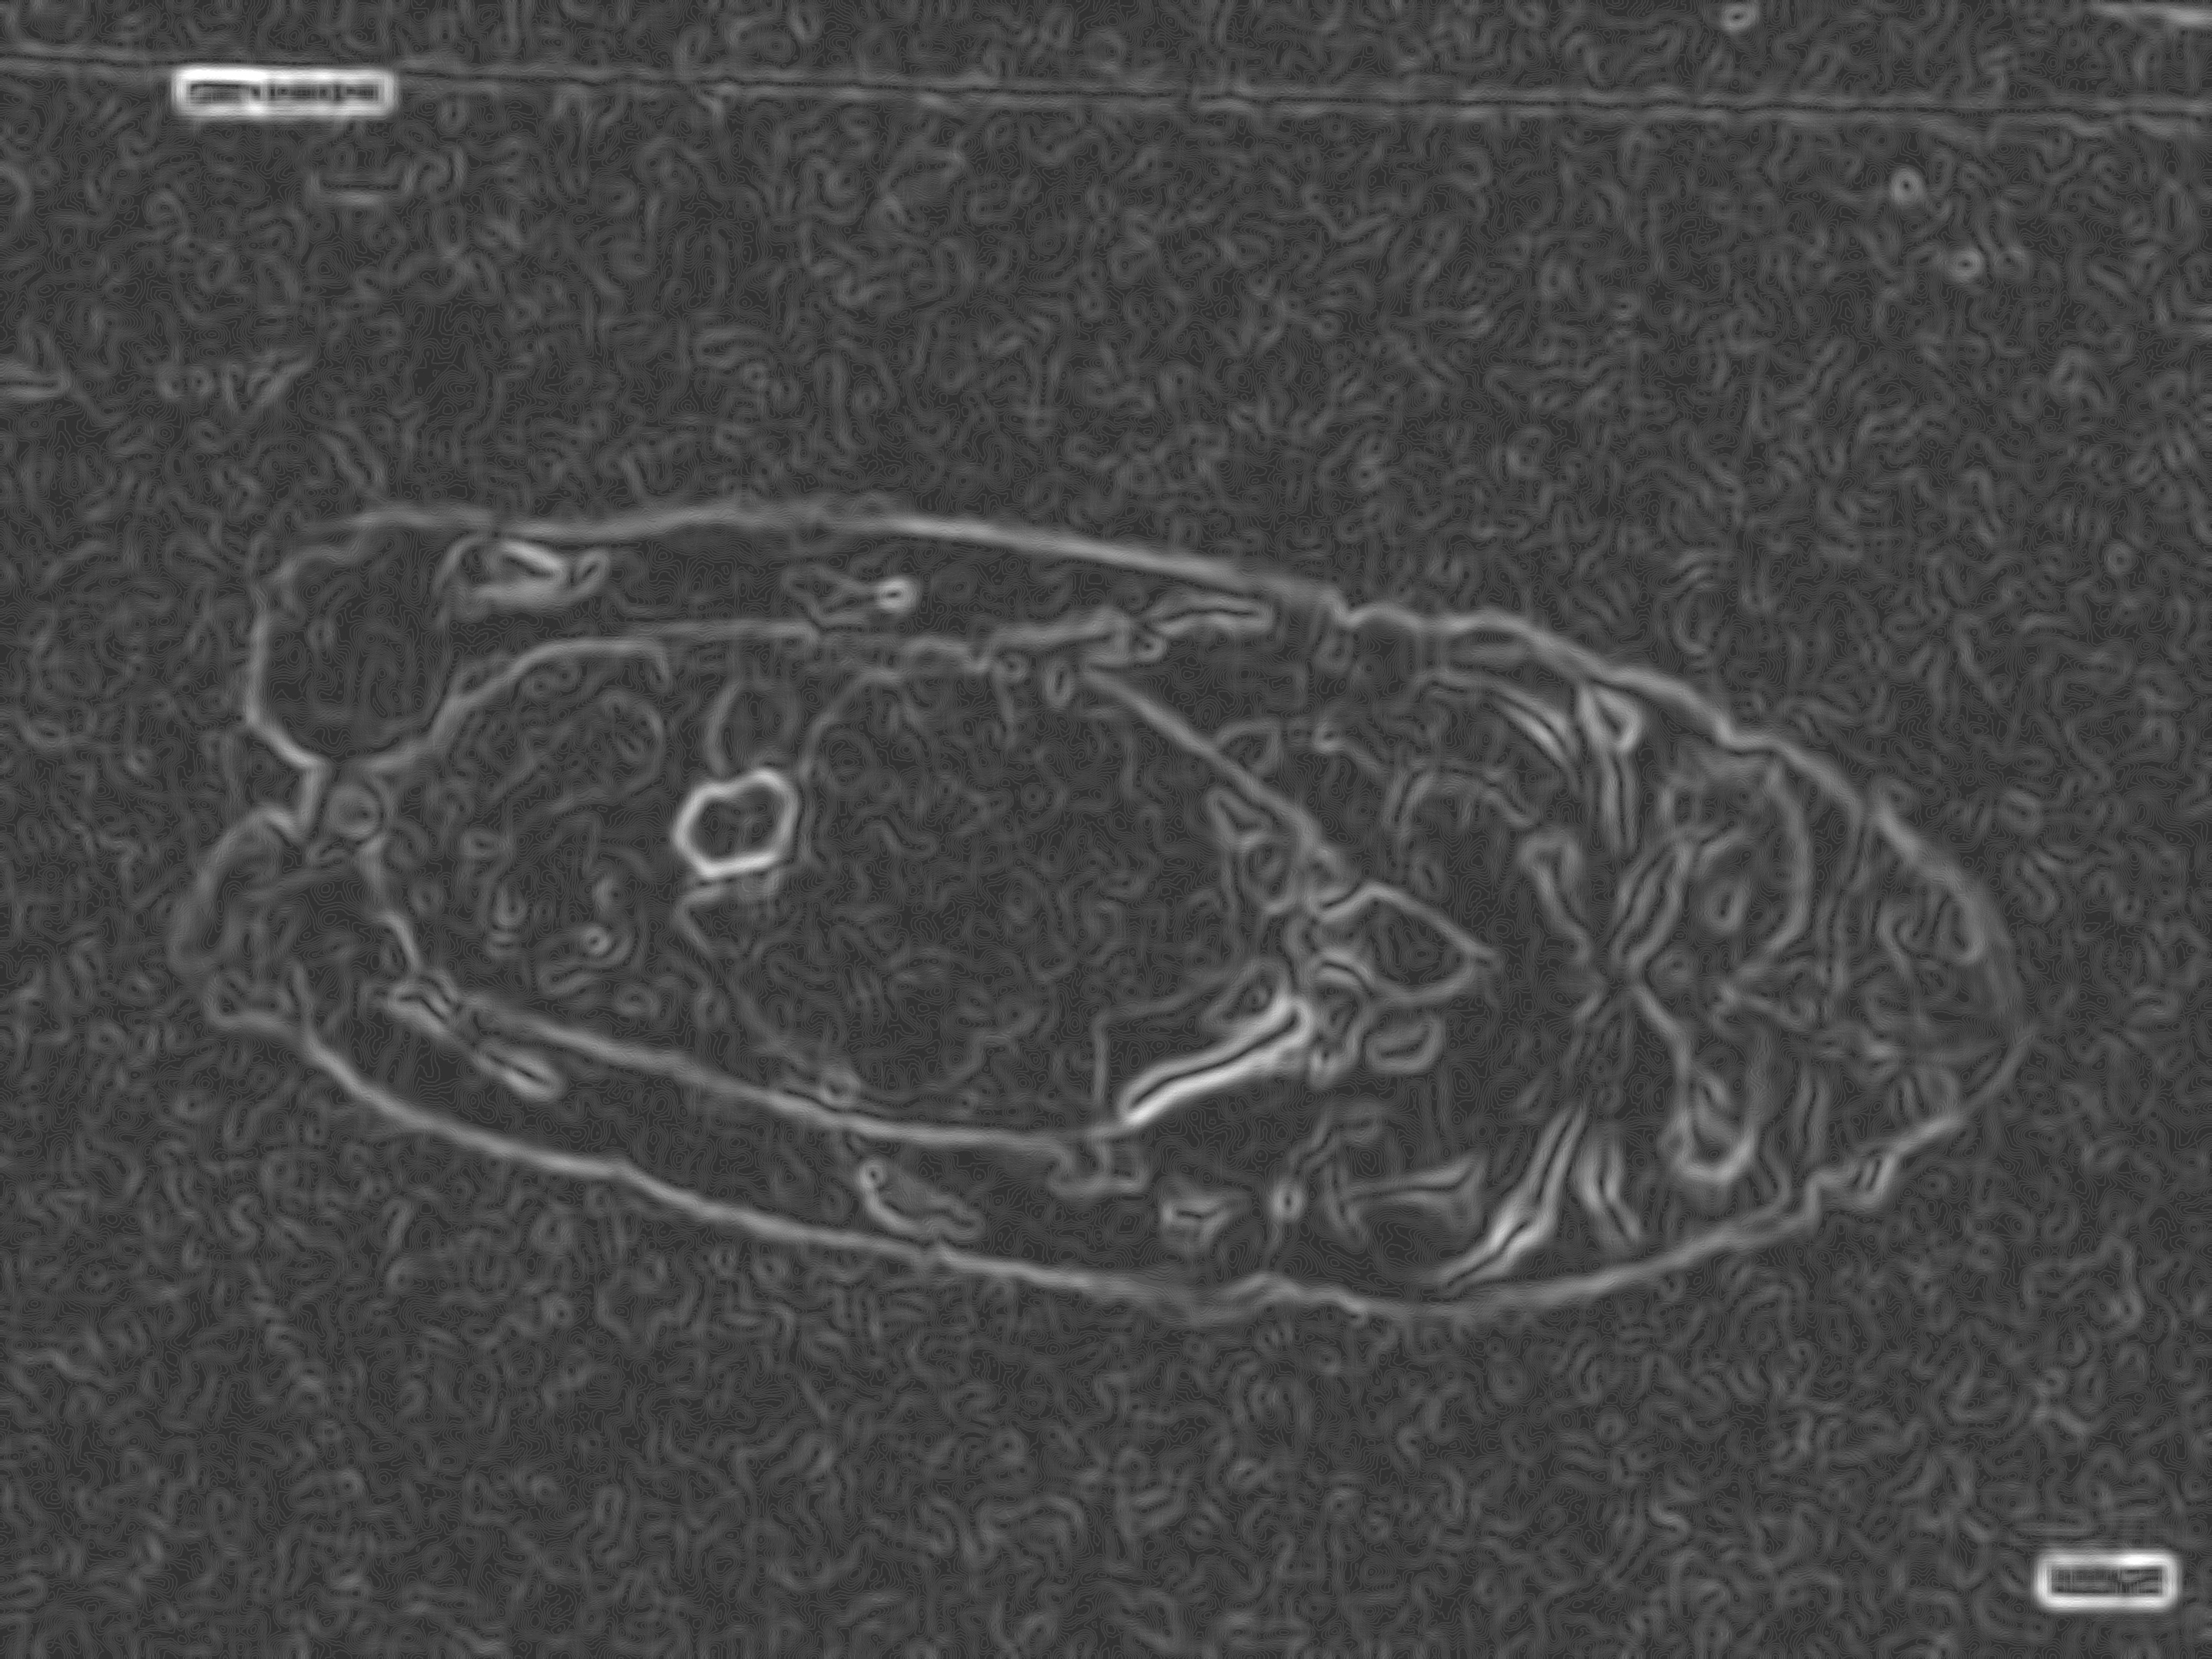
\includegraphics[width=\textwidth]{./fig/gausssian/sobel61.jpg}
        \caption*{k=61}
        \label{fig:sobel61}
    \end{minipage}
    \begin{minipage}{0.24\textwidth}
        \centering
        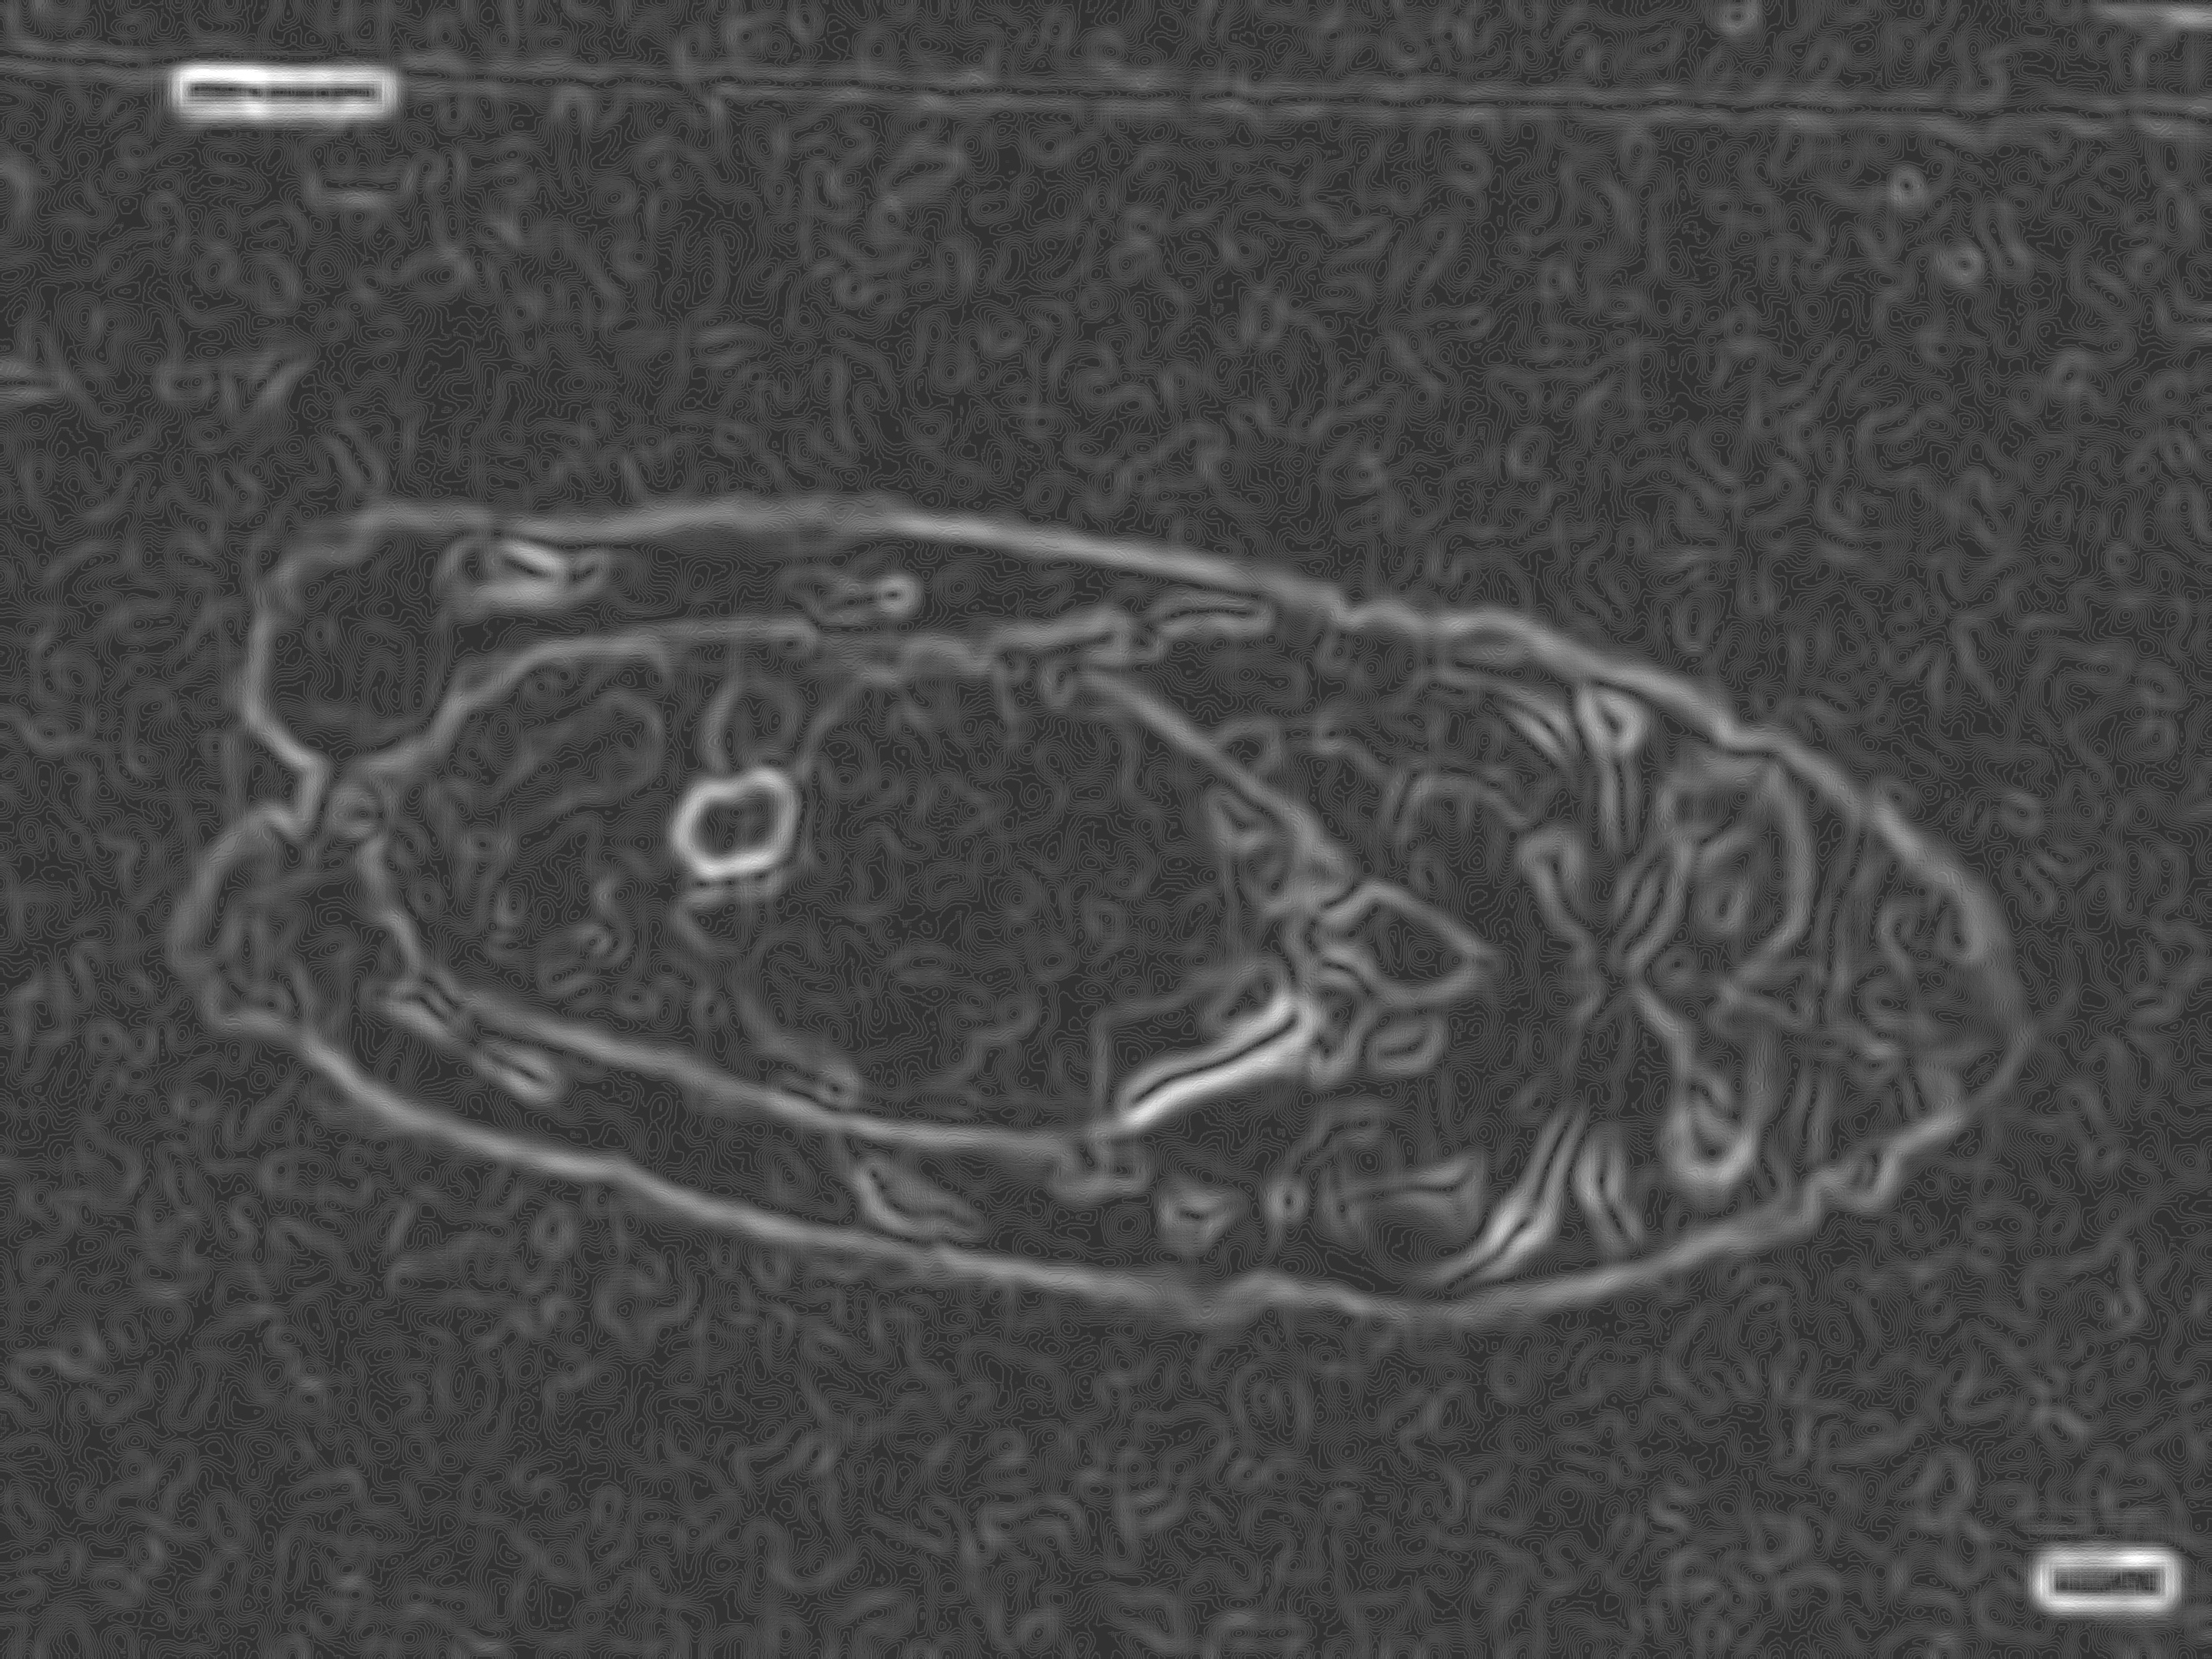
\includegraphics[width=\textwidth]{./fig/gausssian/sobel81.jpg}
        \caption*{k=81}
        \label{fig:sobel81}
    \end{minipage}
    \caption{Images post-Sobel operator}
    \label{fig:sobel}
\end{figure}


在 \autoref{fig:blurred} 中,可以观察到,随着高斯模糊核大小的增加,图像细节逐渐变得更模糊,边缘也变得更不明显。在 \autoref{fig:sobel} 中,随着核大小的增加,边缘检测的效果减弱,边缘变得不那么突出。考虑到图像边缘与背景噪声的清晰度,选择了61的高斯核大小。

应用高斯模糊(k=61)后,使用Python的OpenCV库通过拉普拉斯算子得到的结果如下所示:

\begin{figure}[H]
    \centering
    \begin{minipage}{0.4\textwidth}
        \centering
        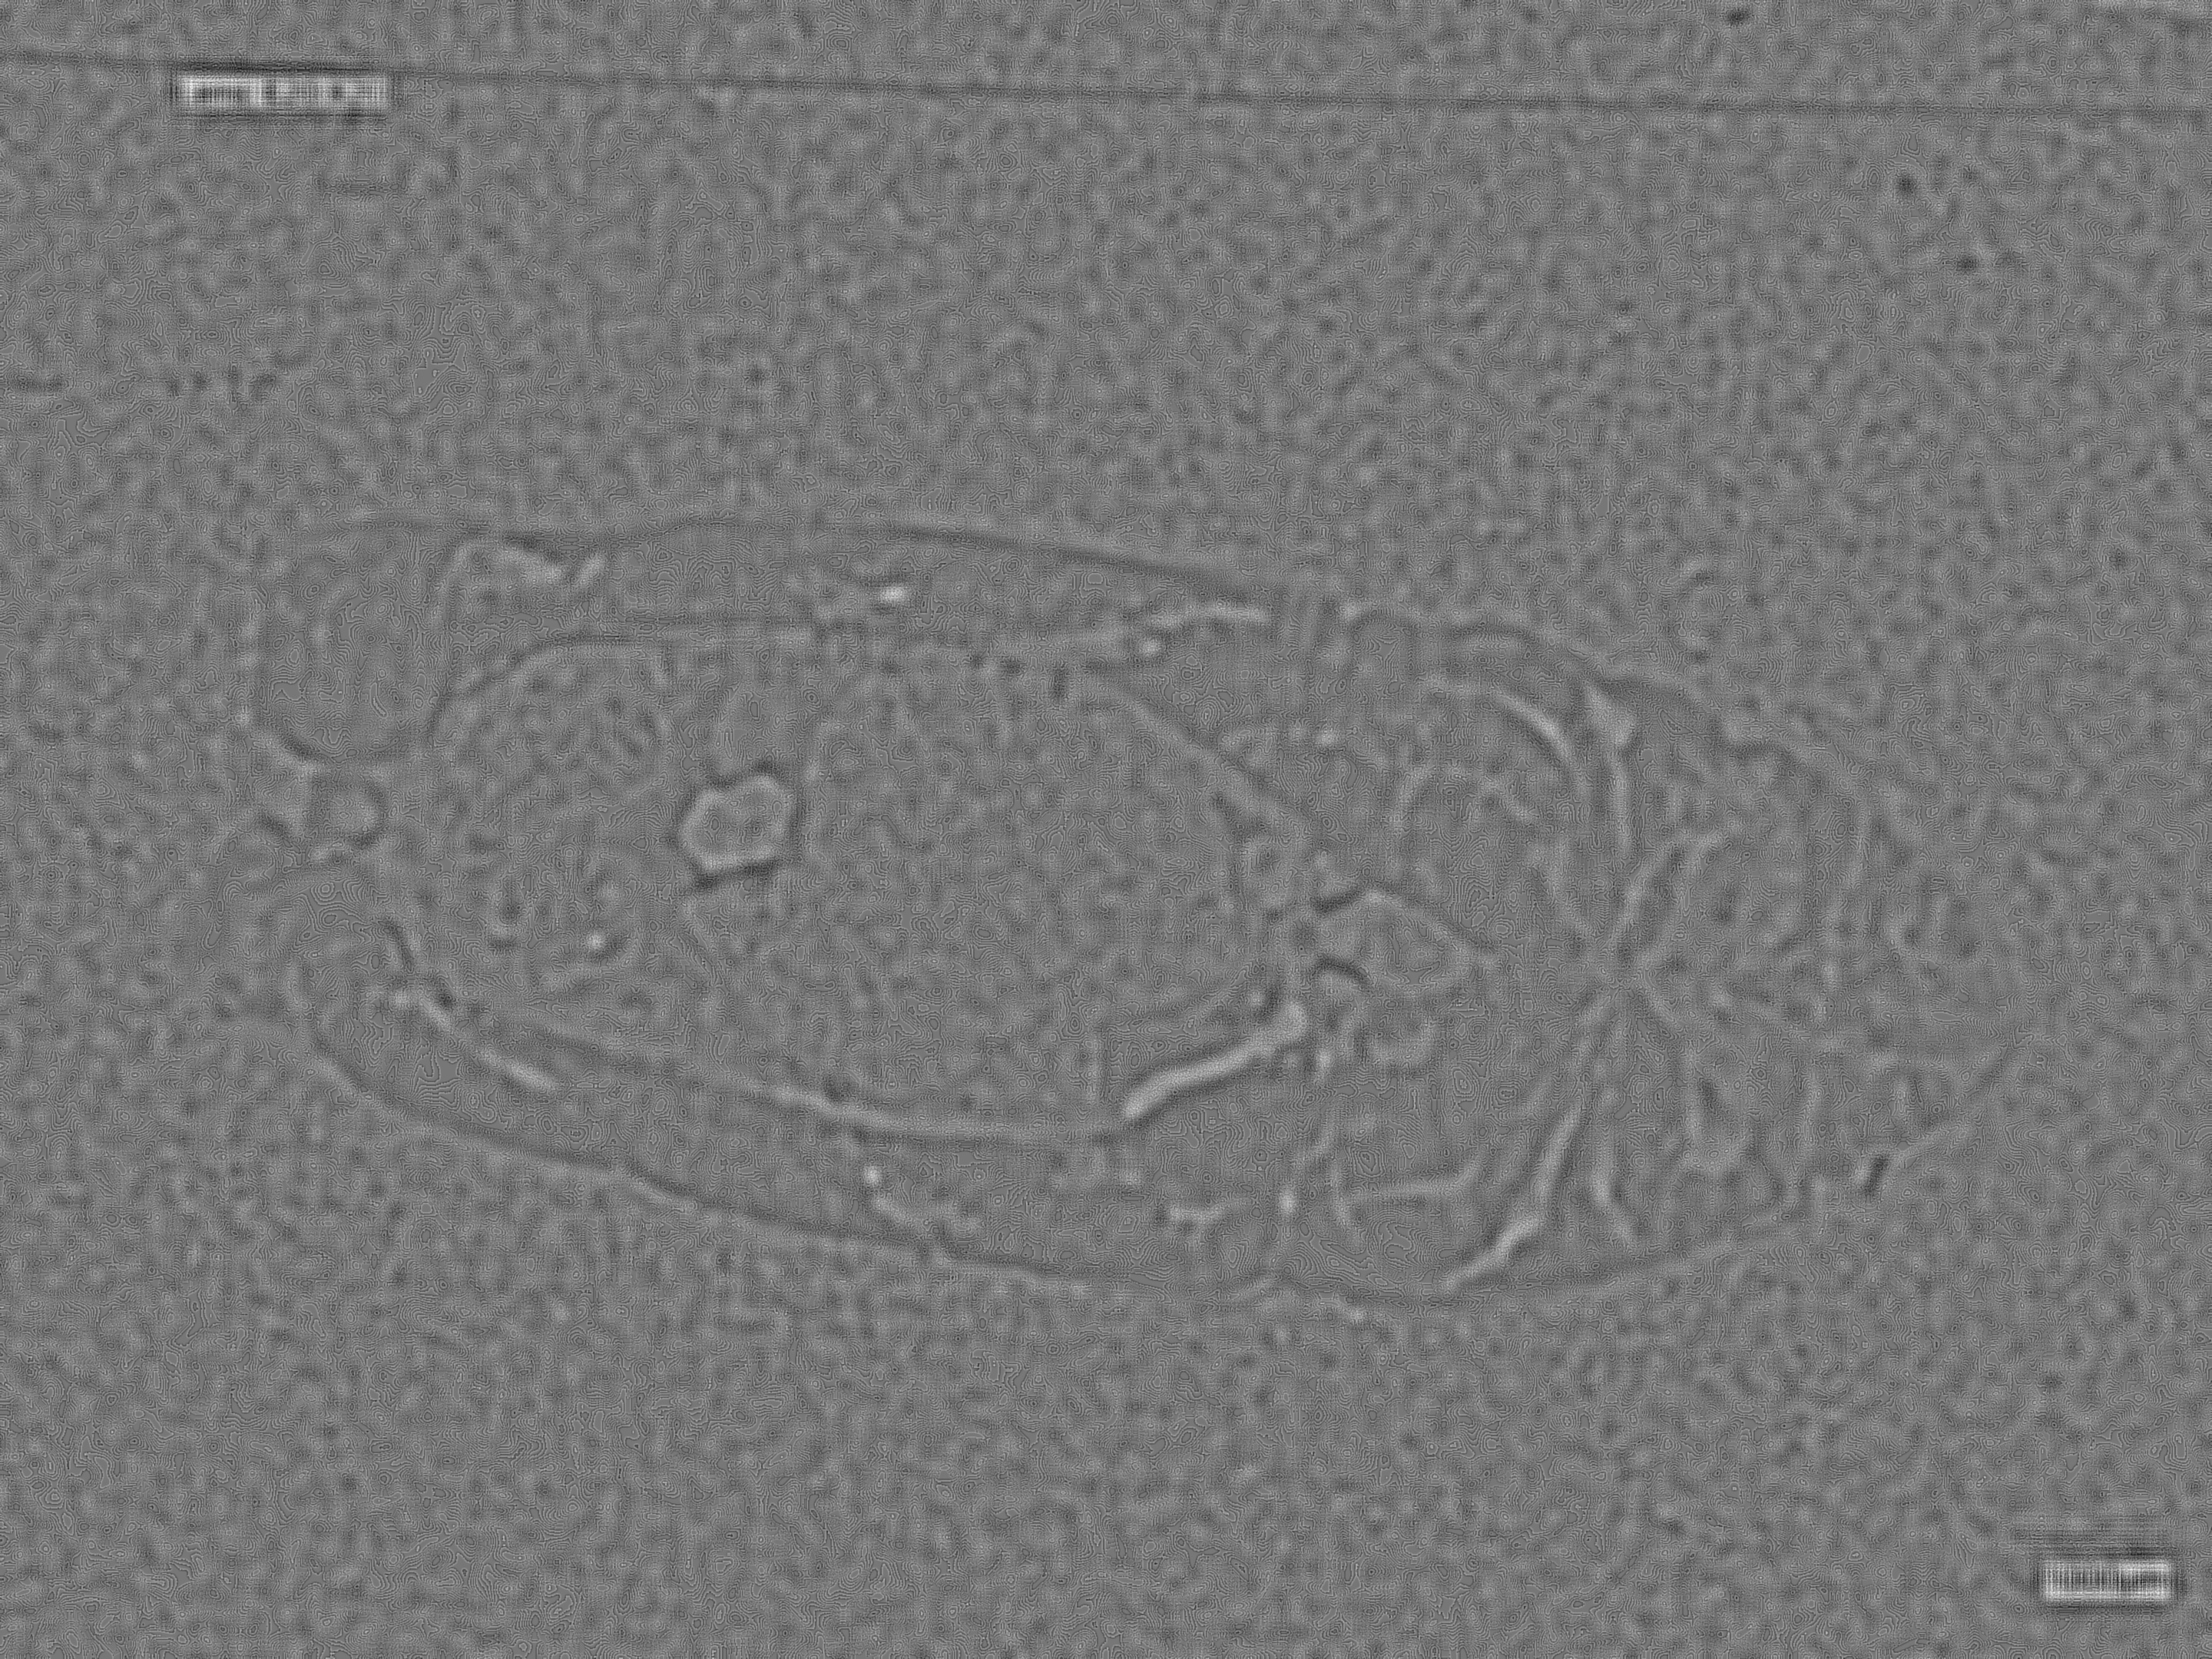
\includegraphics[width=\textwidth]{./fig/gausssian/laplacian61.jpg}
        \caption{laplacian}
        \label{fig:laplacian}
    \end{minipage}
\end{figure}

如前所述,Canny算法比Sobel算法更复杂,包括阈值化和非最大抑制等步骤。Canny方法使用两个阈值,一个低阈值和一个高阈值。大于高阈值的图像梯度被标记为边缘,而低于低阈值的梯度则不被视为边缘。在两个阈值之间的梯度只有在连接到高阈值边缘时才被视为边缘,有效地减少了噪声,从而得到了更准确的边缘检测。

通常,高阈值和低阈值之间的比例在2:1和3:1之间。对于这个实验,选择了2.5:1的比例,并探索了不同阈值对边缘检测的影响。

选择的低阈值是2、4和6,对应的高阈值分别是5、10和15。Canny算法的结果如下所示:

\begin{figure}
    \centering
    \begin{minipage}{0.32\textwidth}
        \centering
        \includegraphics[width=\textwidth]{./fig/gausssian/canny61+2.jpg}
        \caption{canny 2 5}
        \label{fig:canny2_5}
    \end{minipage}
    \begin{minipage}{0.32\textwidth}
        \centering
        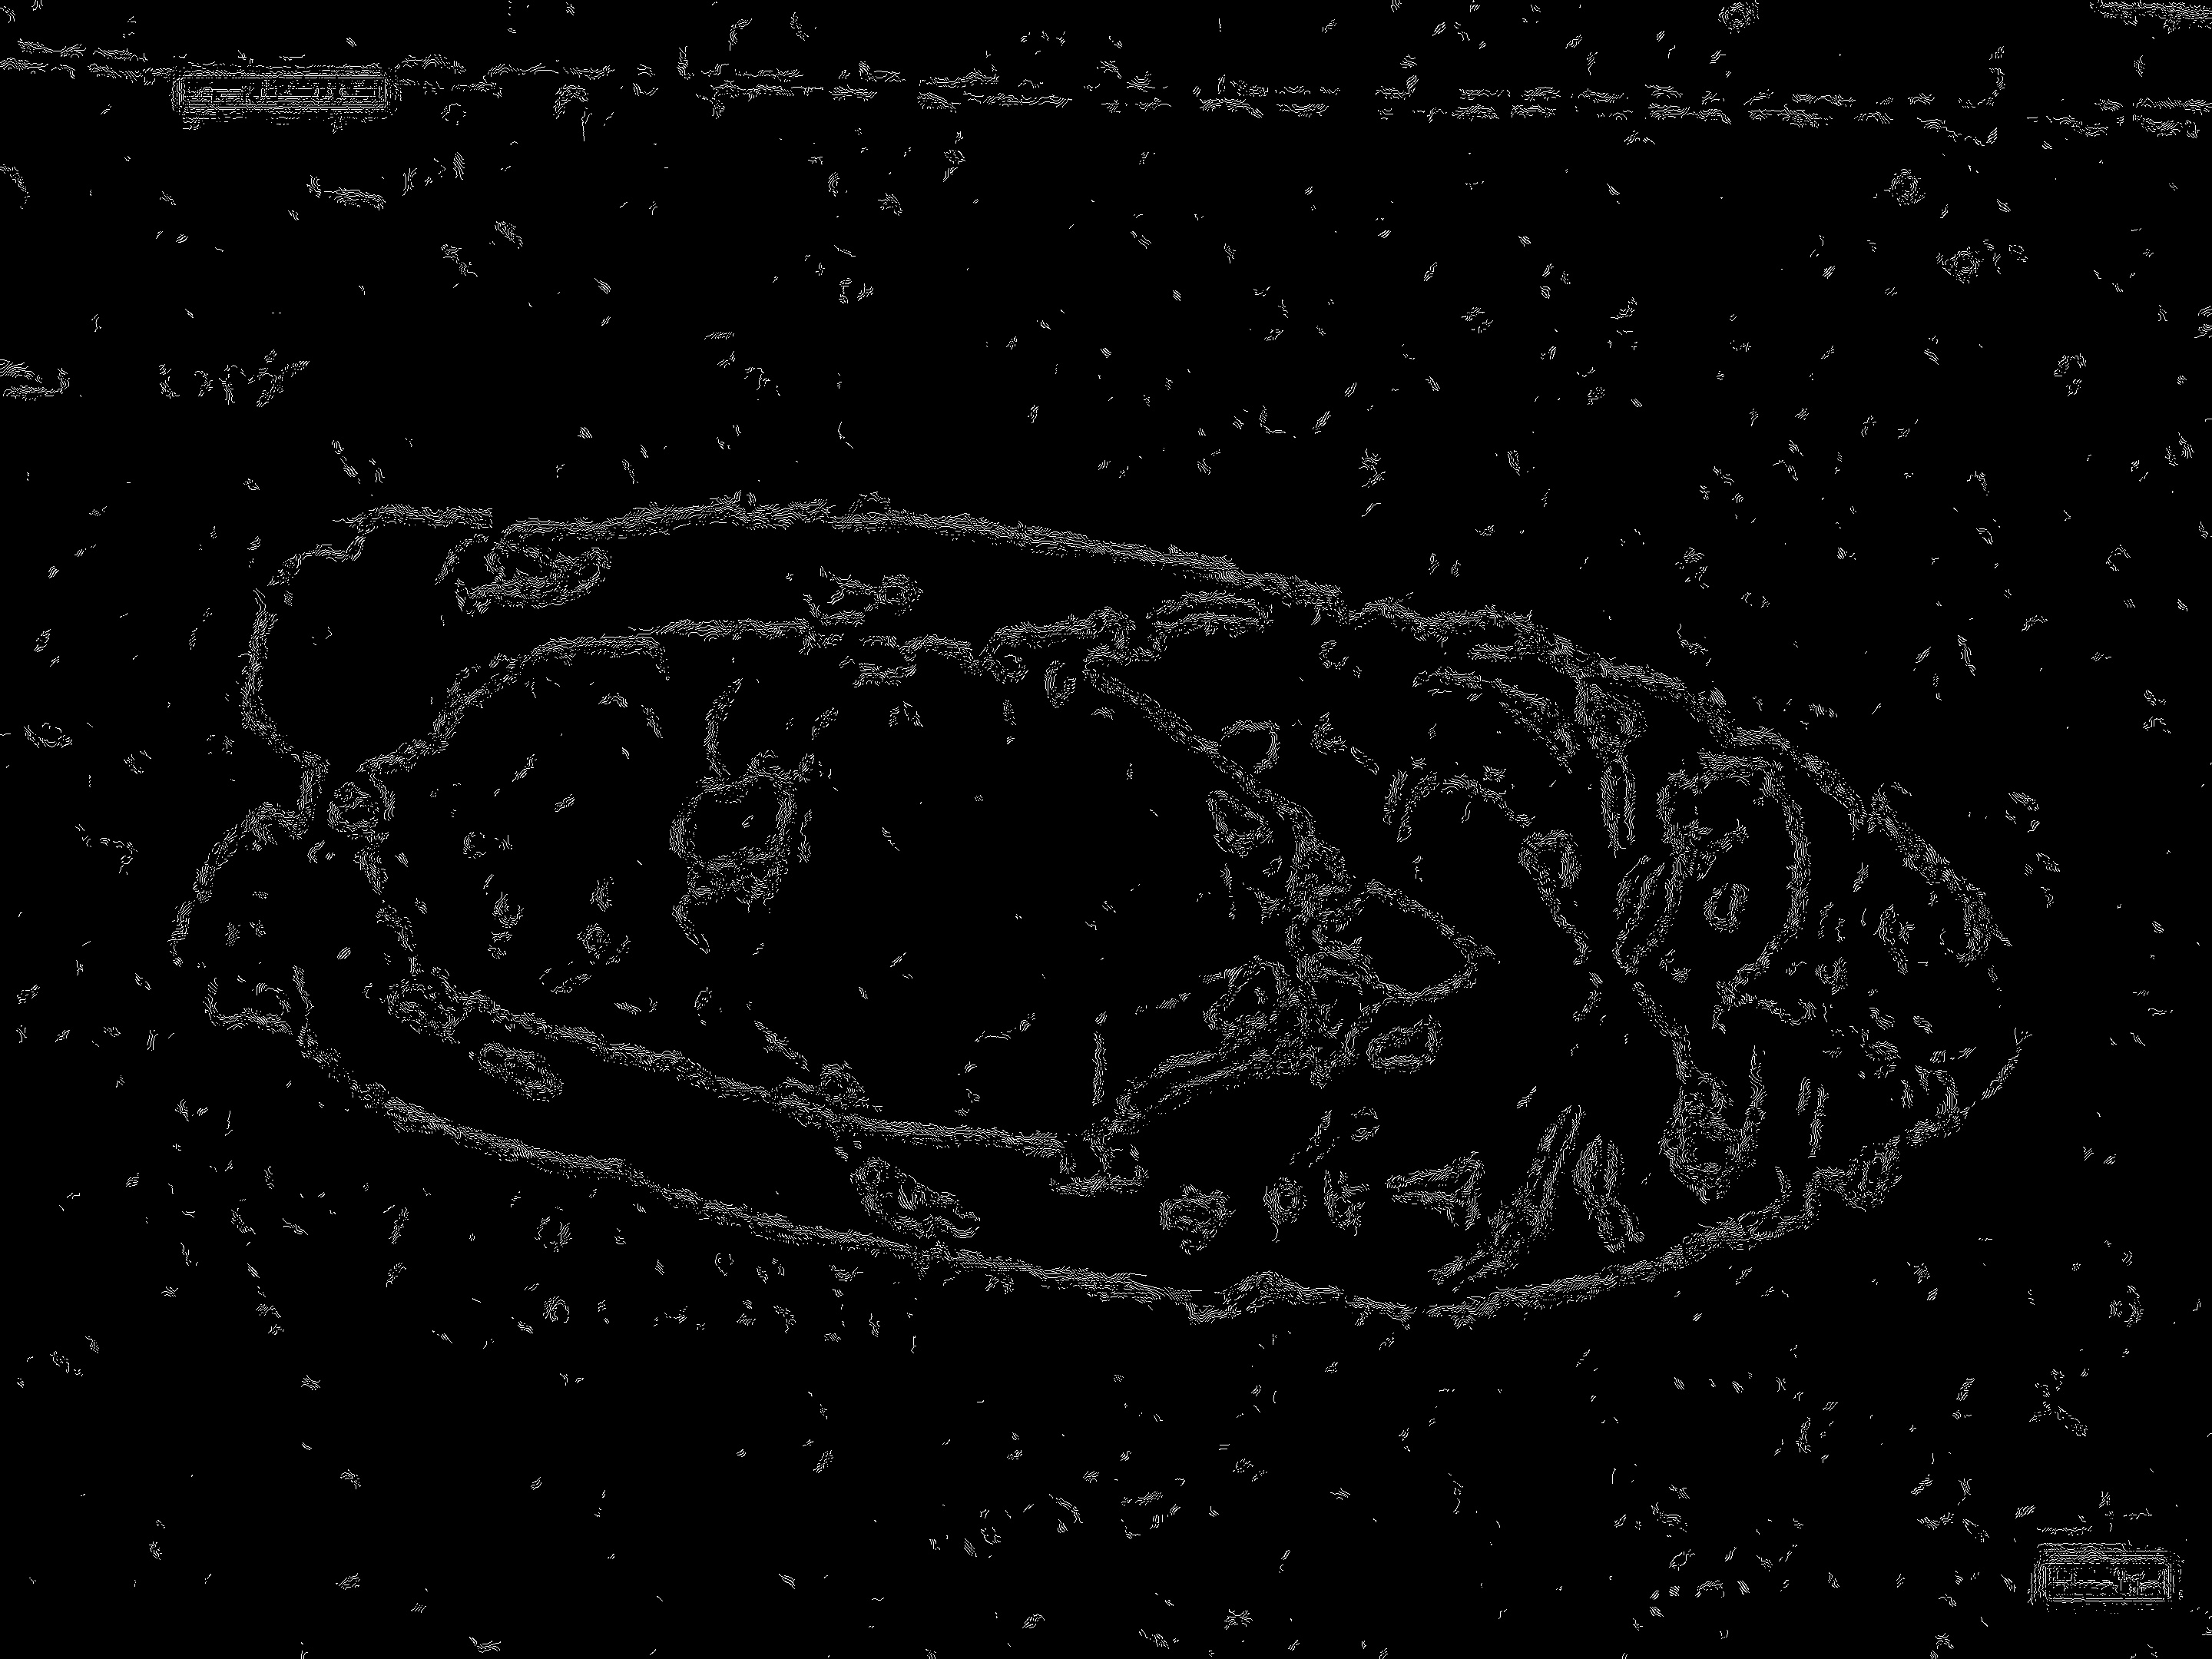
\includegraphics[width=\textwidth]{./fig/gausssian/canny61+4.jpg}
        \caption{canny 4 10}
        \label{fig:canny4_10}
    \end{minipage}
    \begin{minipage}{0.32\textwidth}
        \centering
        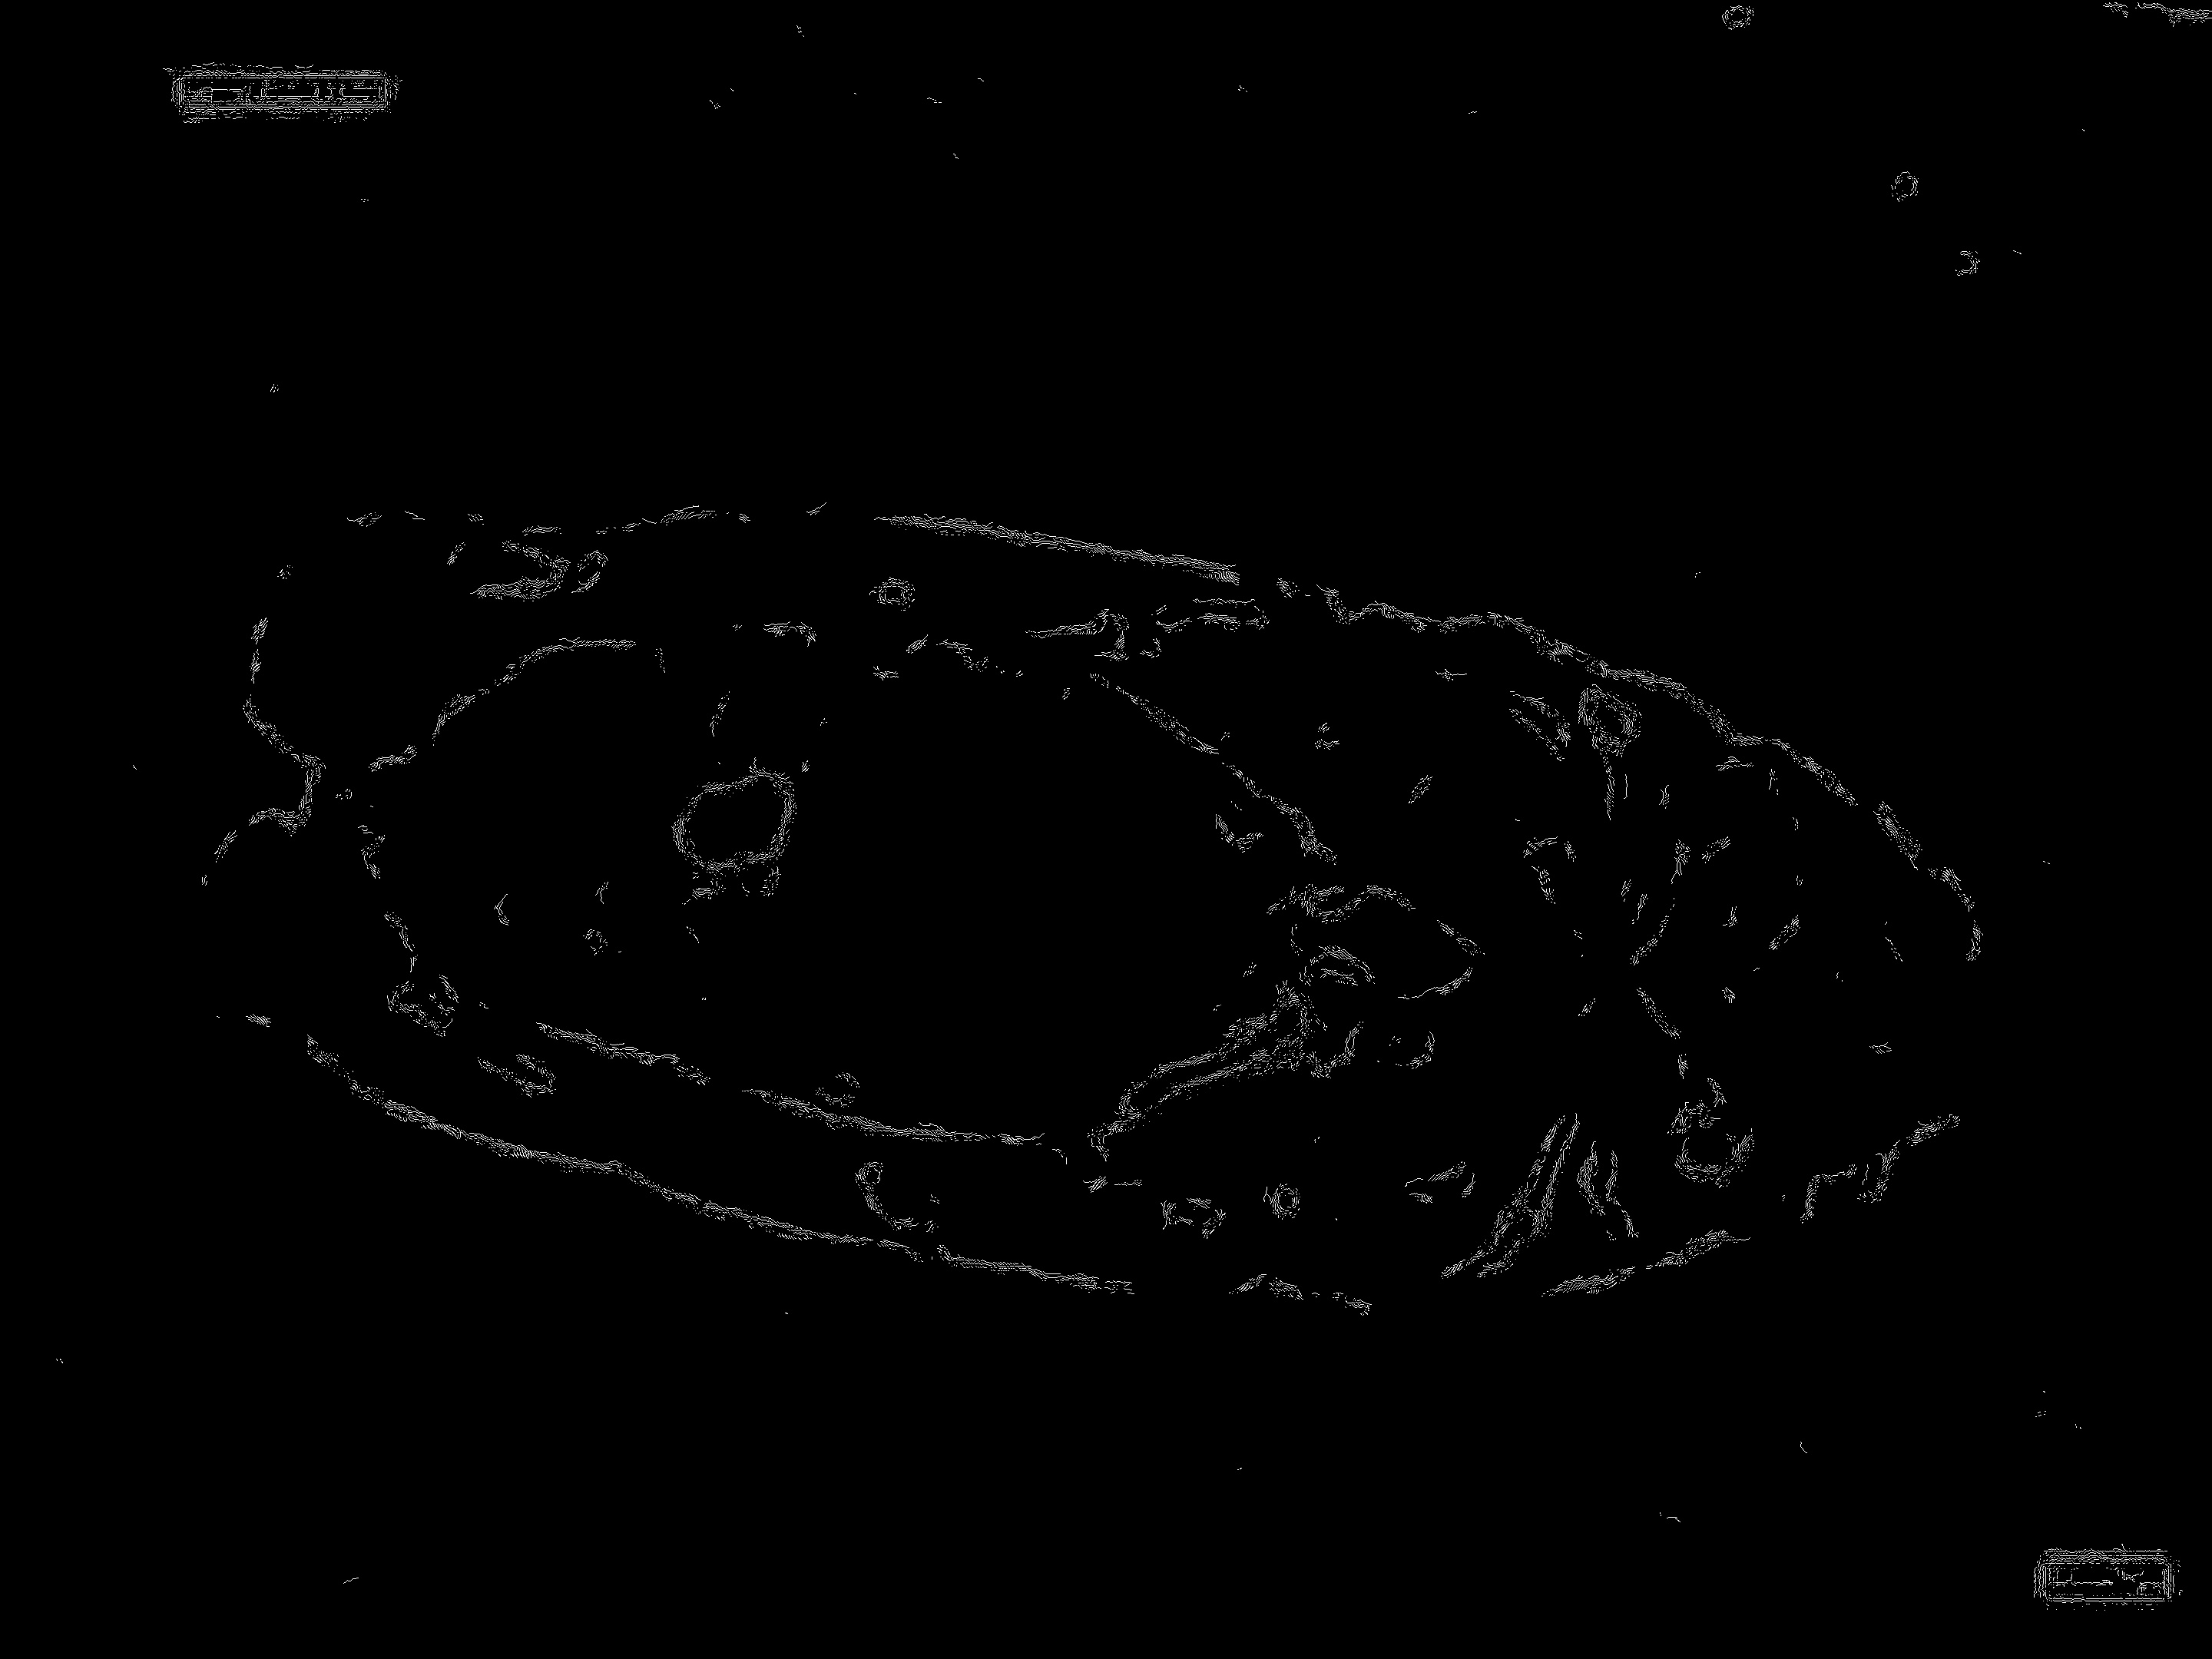
\includegraphics[width=\textwidth]{./fig/gausssian/canny61+6.jpg}
        \caption{canny 6 15}
        \label{fig:canny6_15}
    \end{minipage}
\end{figure}


在三个Canny结果中,\autoref{fig:canny4_10} 的表现最好,能够保留大部分边缘细节,同时有效地消除了大部分噪声。因此,选择了4和10作为Canny算法的阈值。

\textbf{总结}

比较Sobel、Laplacian和Canny算法的结果,Sobel算法的表现一般,边缘检测明显,但噪声减少有限。Laplacian算法的表现最差,边缘几乎变得不可见,可能是由于其对噪声的高敏感度。Canny算法的结果最好,保持了边缘细节,同时有效地去除了大部分噪声。因此,选择Canny算法作为图像预处理的方法,增强了模型对于进一步分析的相关特征的关注能力。

\subsubsection{Threshold Segmentation}
考虑到生物组织样本(黄色)和标本中的石蜡(白色)的颜色差异,阈值分割提供了一种直接的方法来区分这两个组成部分,通过隔离图像的白色区域,保留生物组织。这个过程包括增强图像的对比度和饱和度,以更好地突出生物组织的黄色,如 \autoref{fig:enhanced_image} 所示。处理步骤使用 Python 的 OpenCV 库执行。

首先,评估图像中的每个像素,保留黄色像素周围大约半径 15(约为图像宽度的 1\%)的像素。其他颜色被移除,如 \autoref{fig:yellowpic} 所示。然而,由于切割过程中组织碎片的分散,这种方法显示出了限制,这些碎片可能散布在整个标本中,干扰了黄色像素的检测。

\begin{figure}[H]
    \centering
    \begin{minipage}{0.40\textwidth}
        \centering
        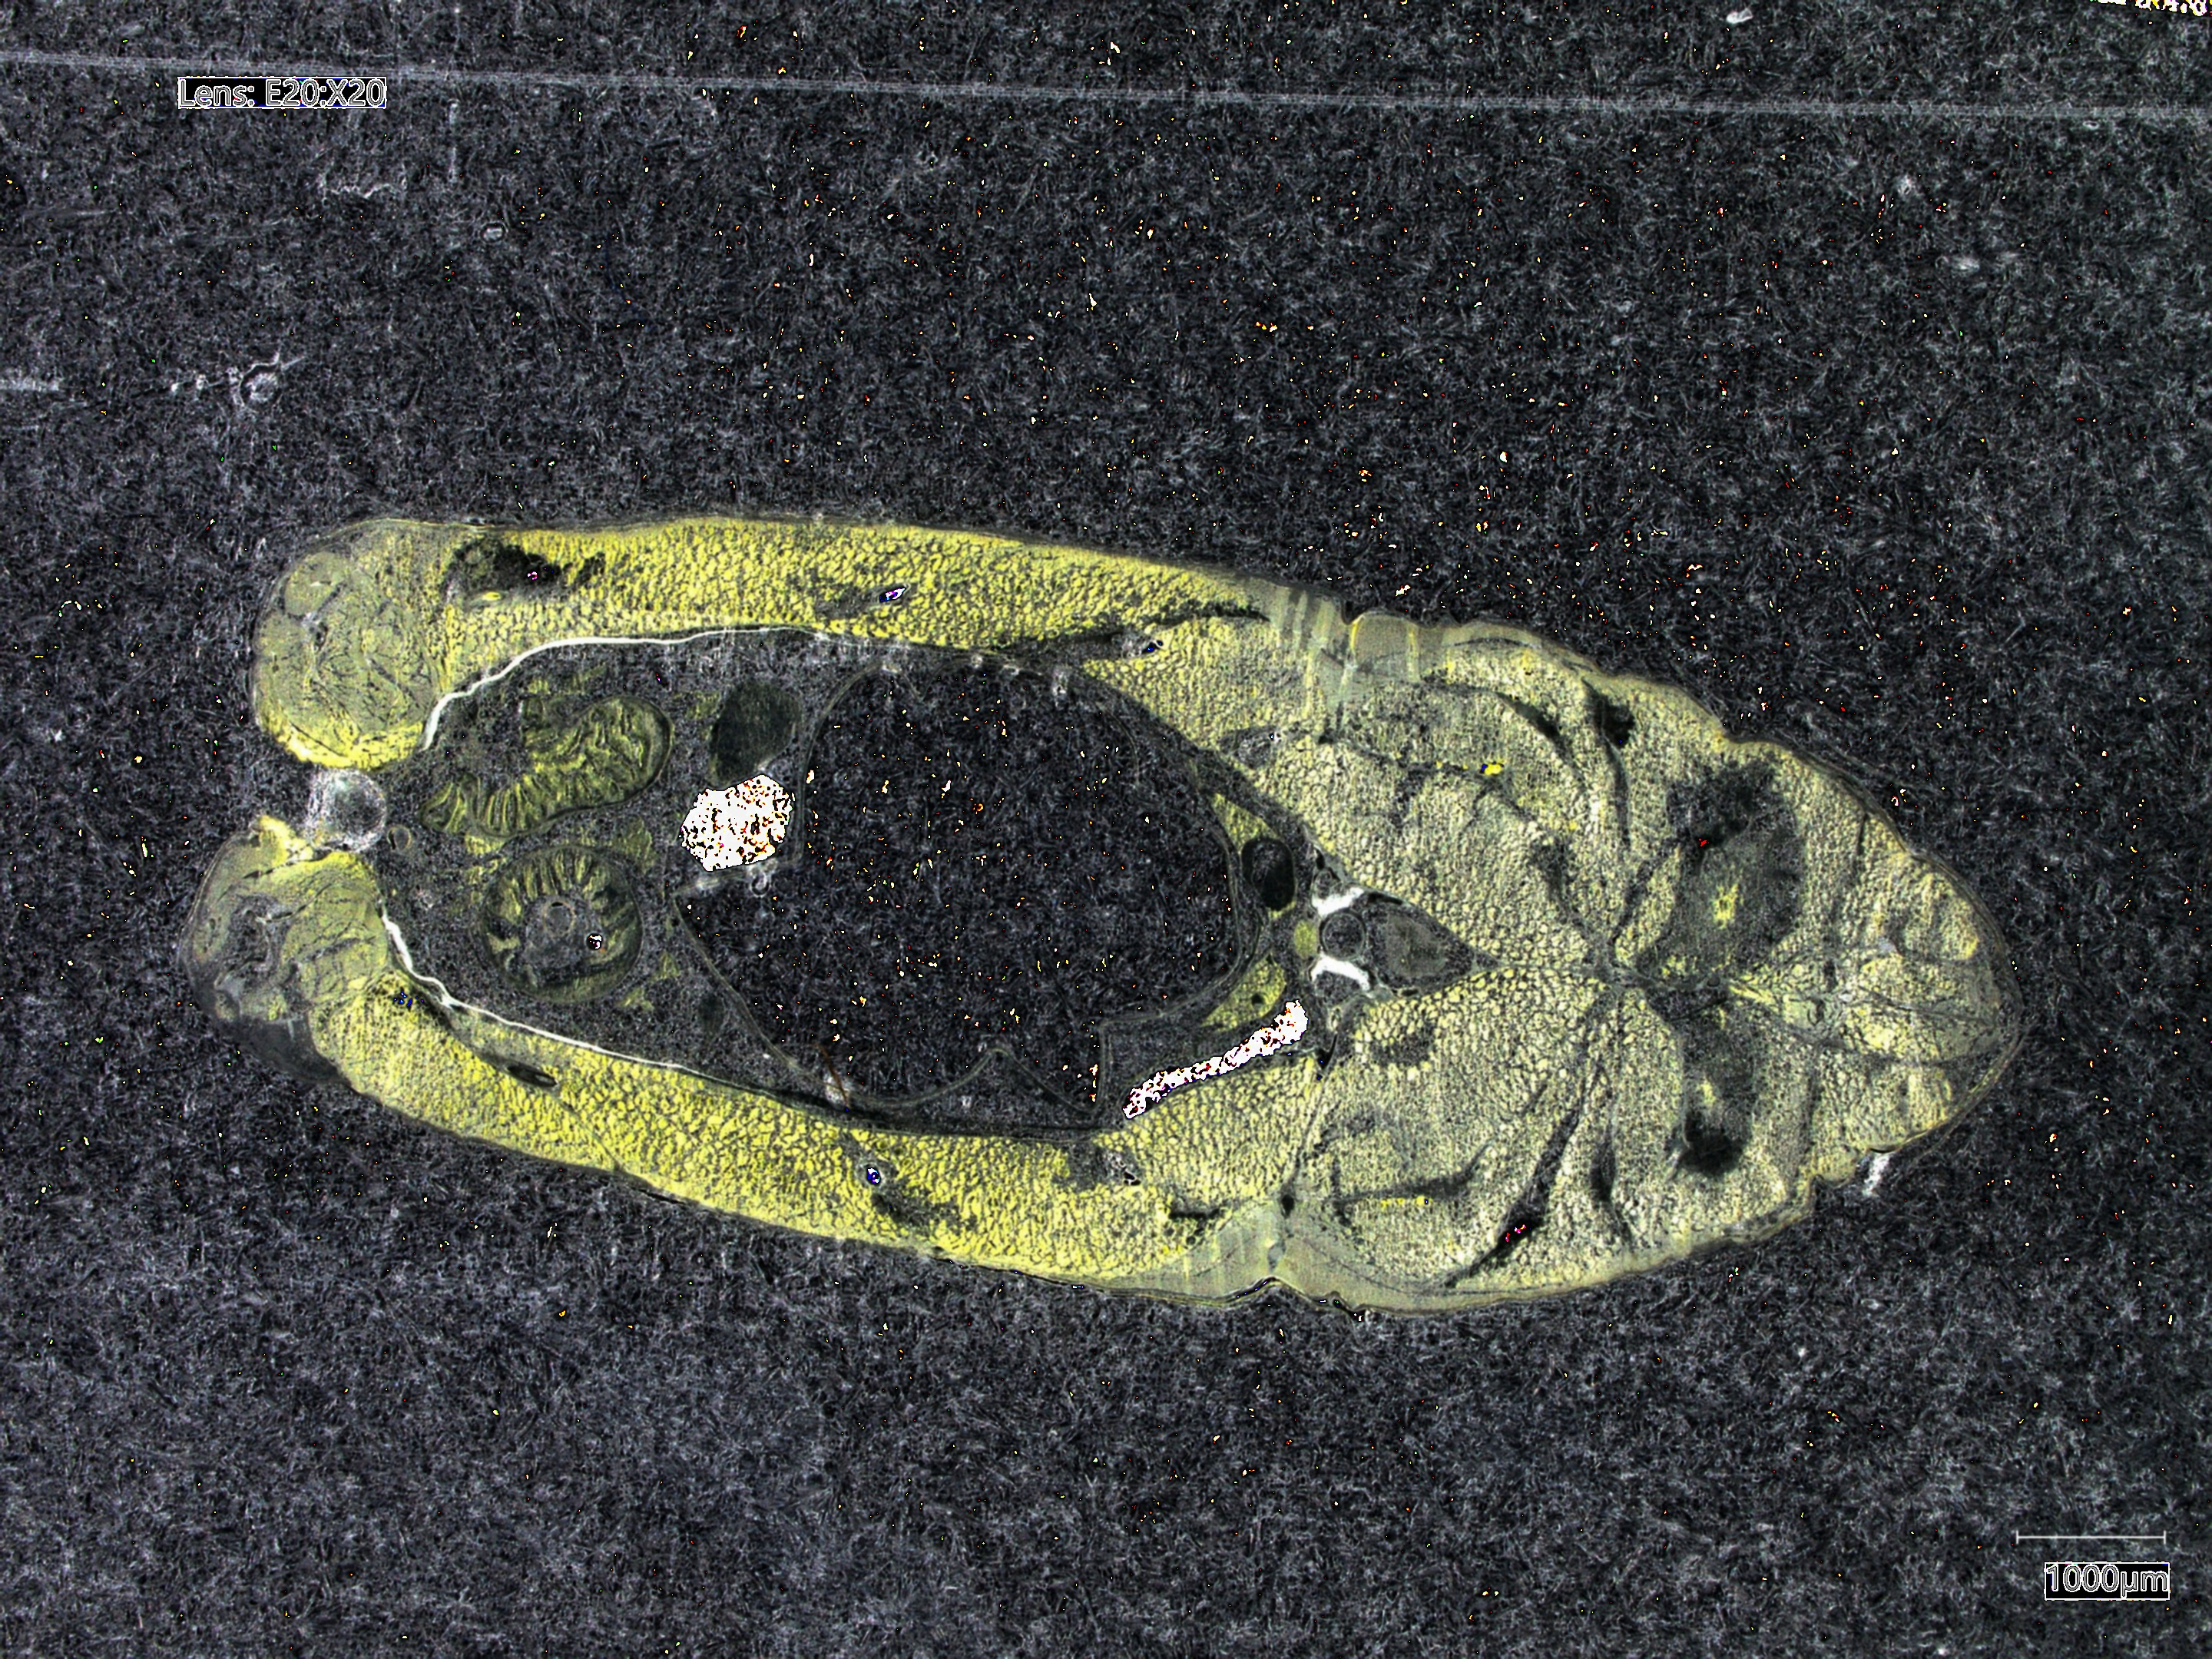
\includegraphics[width=\textwidth]{./fig/threshold/enhanced_image.jpg}
        \caption{增强了颜色区分的图像}
        \label{fig:enhanced_image}
    \end{minipage}
    \begin{minipage}{0.4\textwidth}
        \centering
        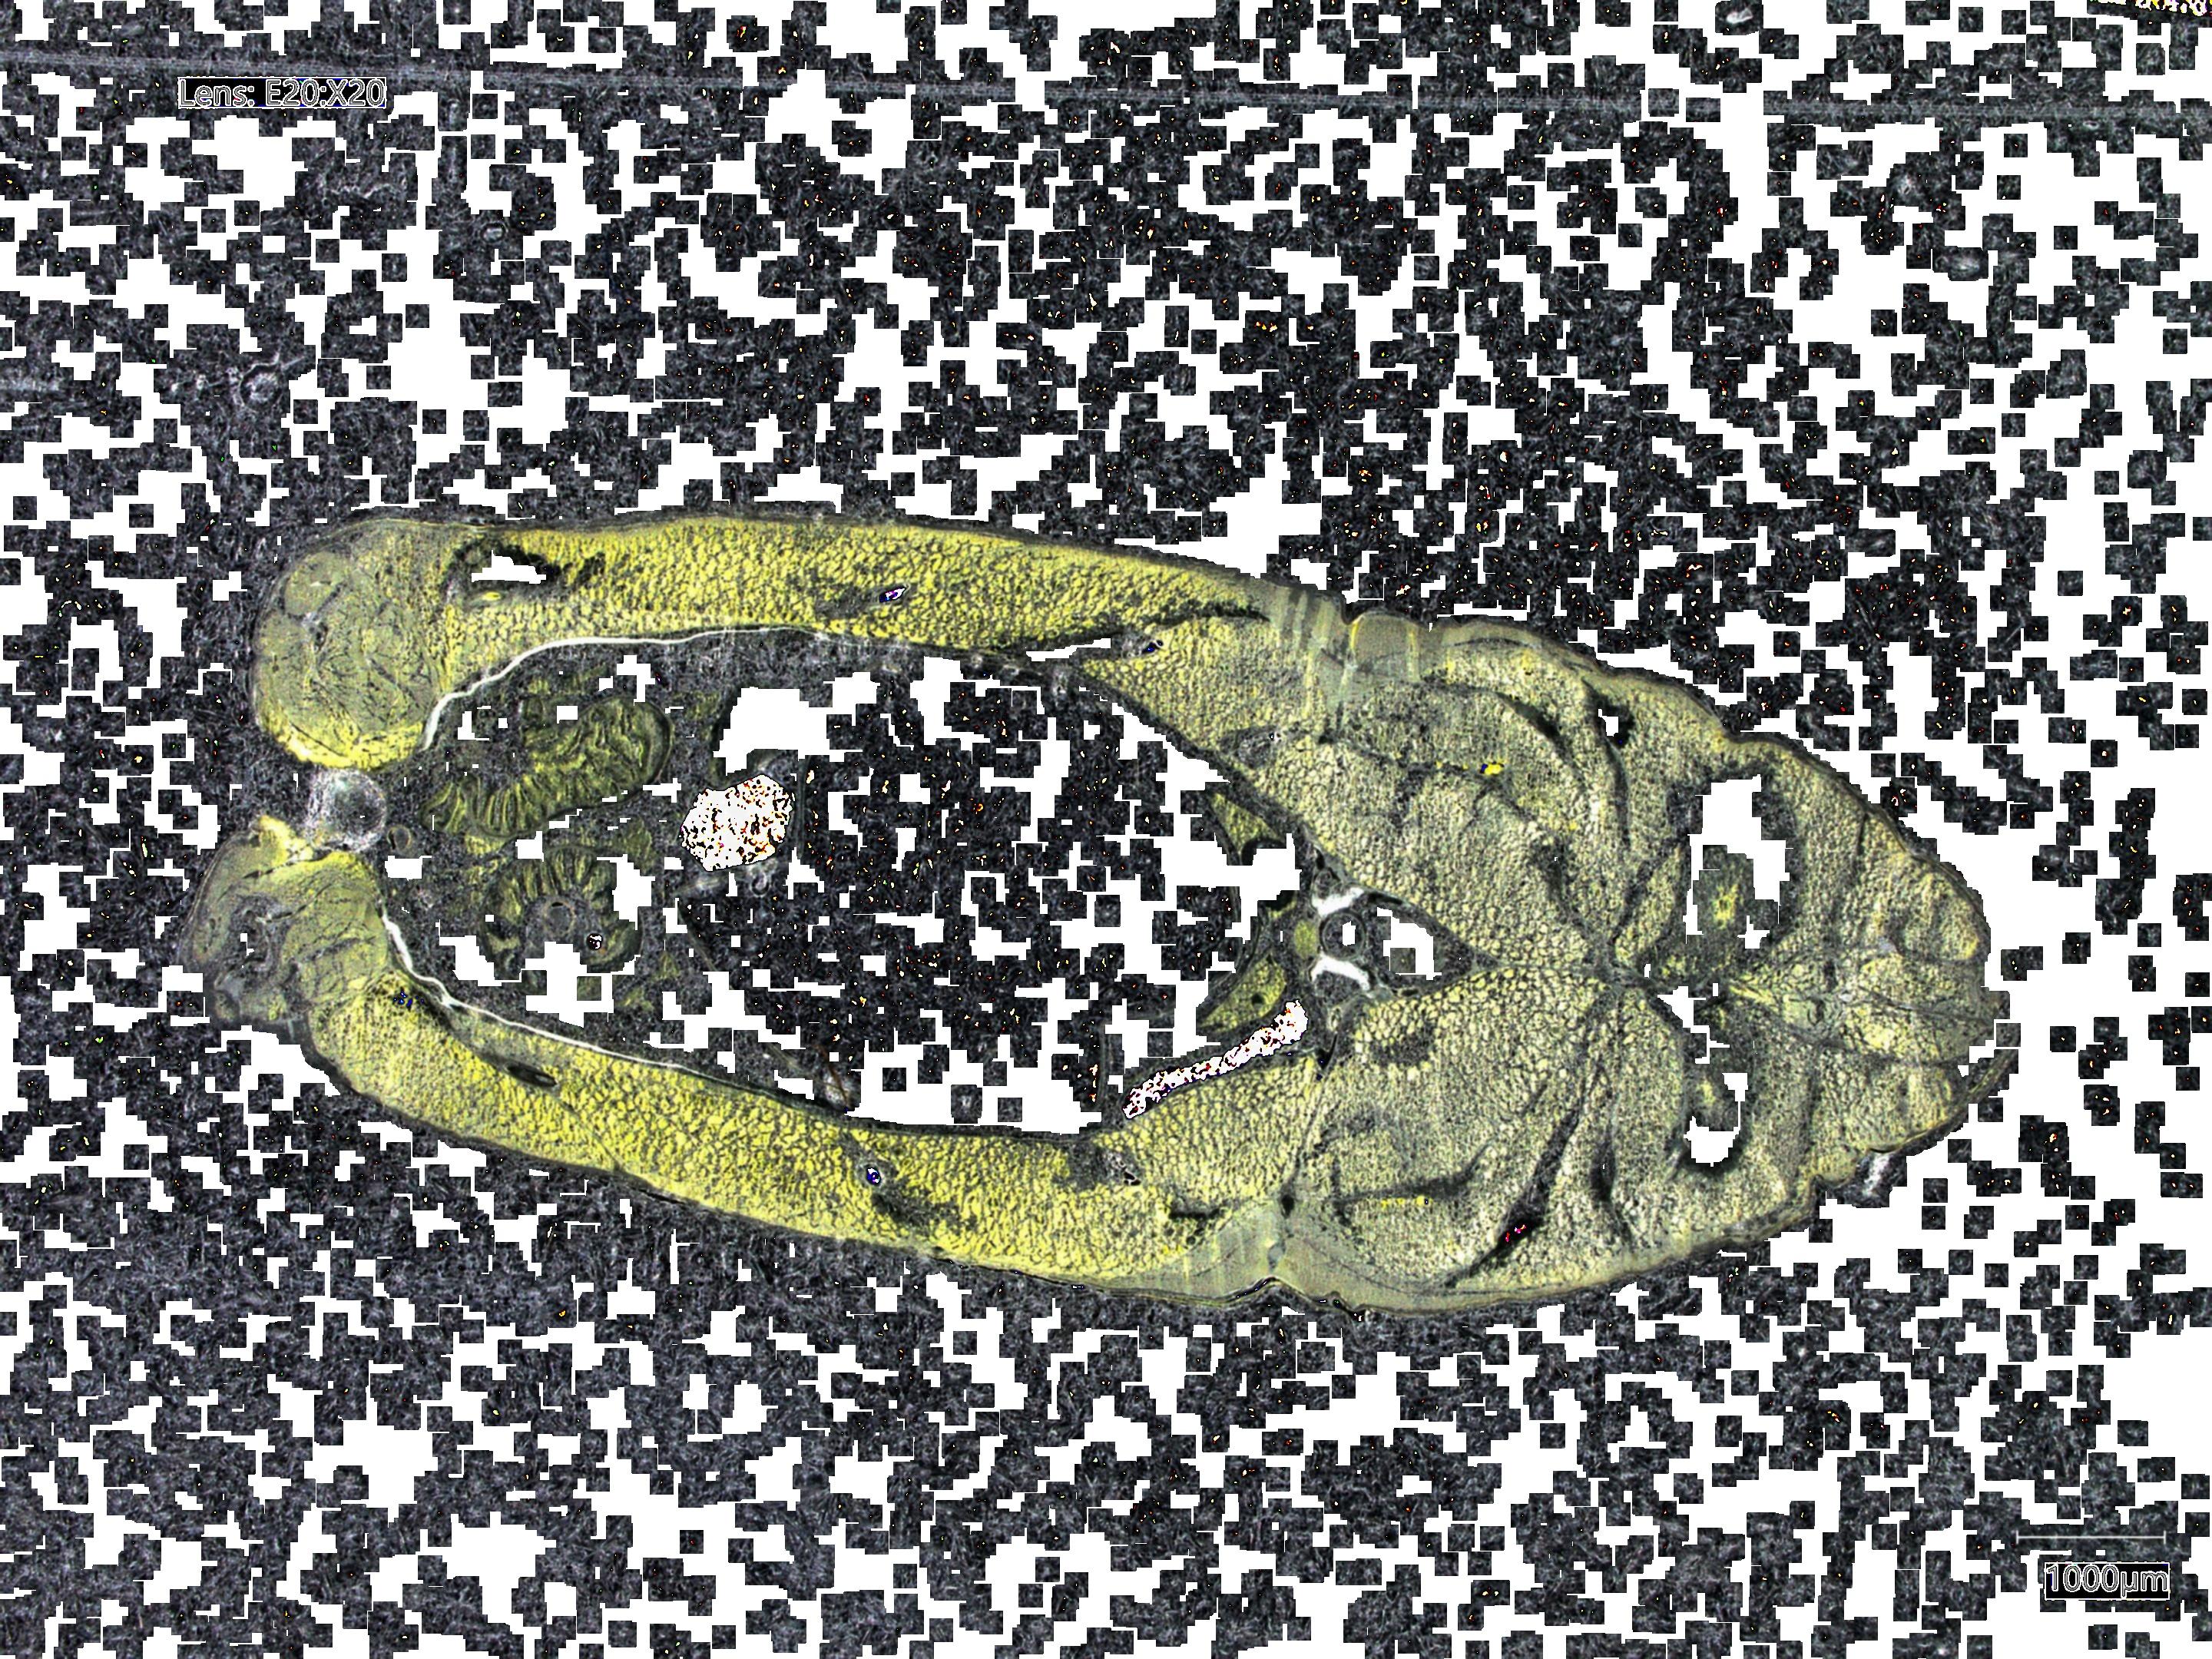
\includegraphics[width=\textwidth]{./fig/threshold/yellowpic.jpg}
        \caption{聚焦于黄色像素的分割}
        \label{fig:yellowpic}
    \end{minipage}
\end{figure}

为了精细化分割,需要进一步处理以消除图像中出现的黑色块。这是通过应用掩码反转来实现的,将这些黑色块变成白色,从而增强了生物组织与石蜡基底的分离。结果显示在 \autoref{fig:mask} 中。

\begin{figure}[H]
    \centering
    \begin{minipage}{0.4\textwidth}
        \centering
        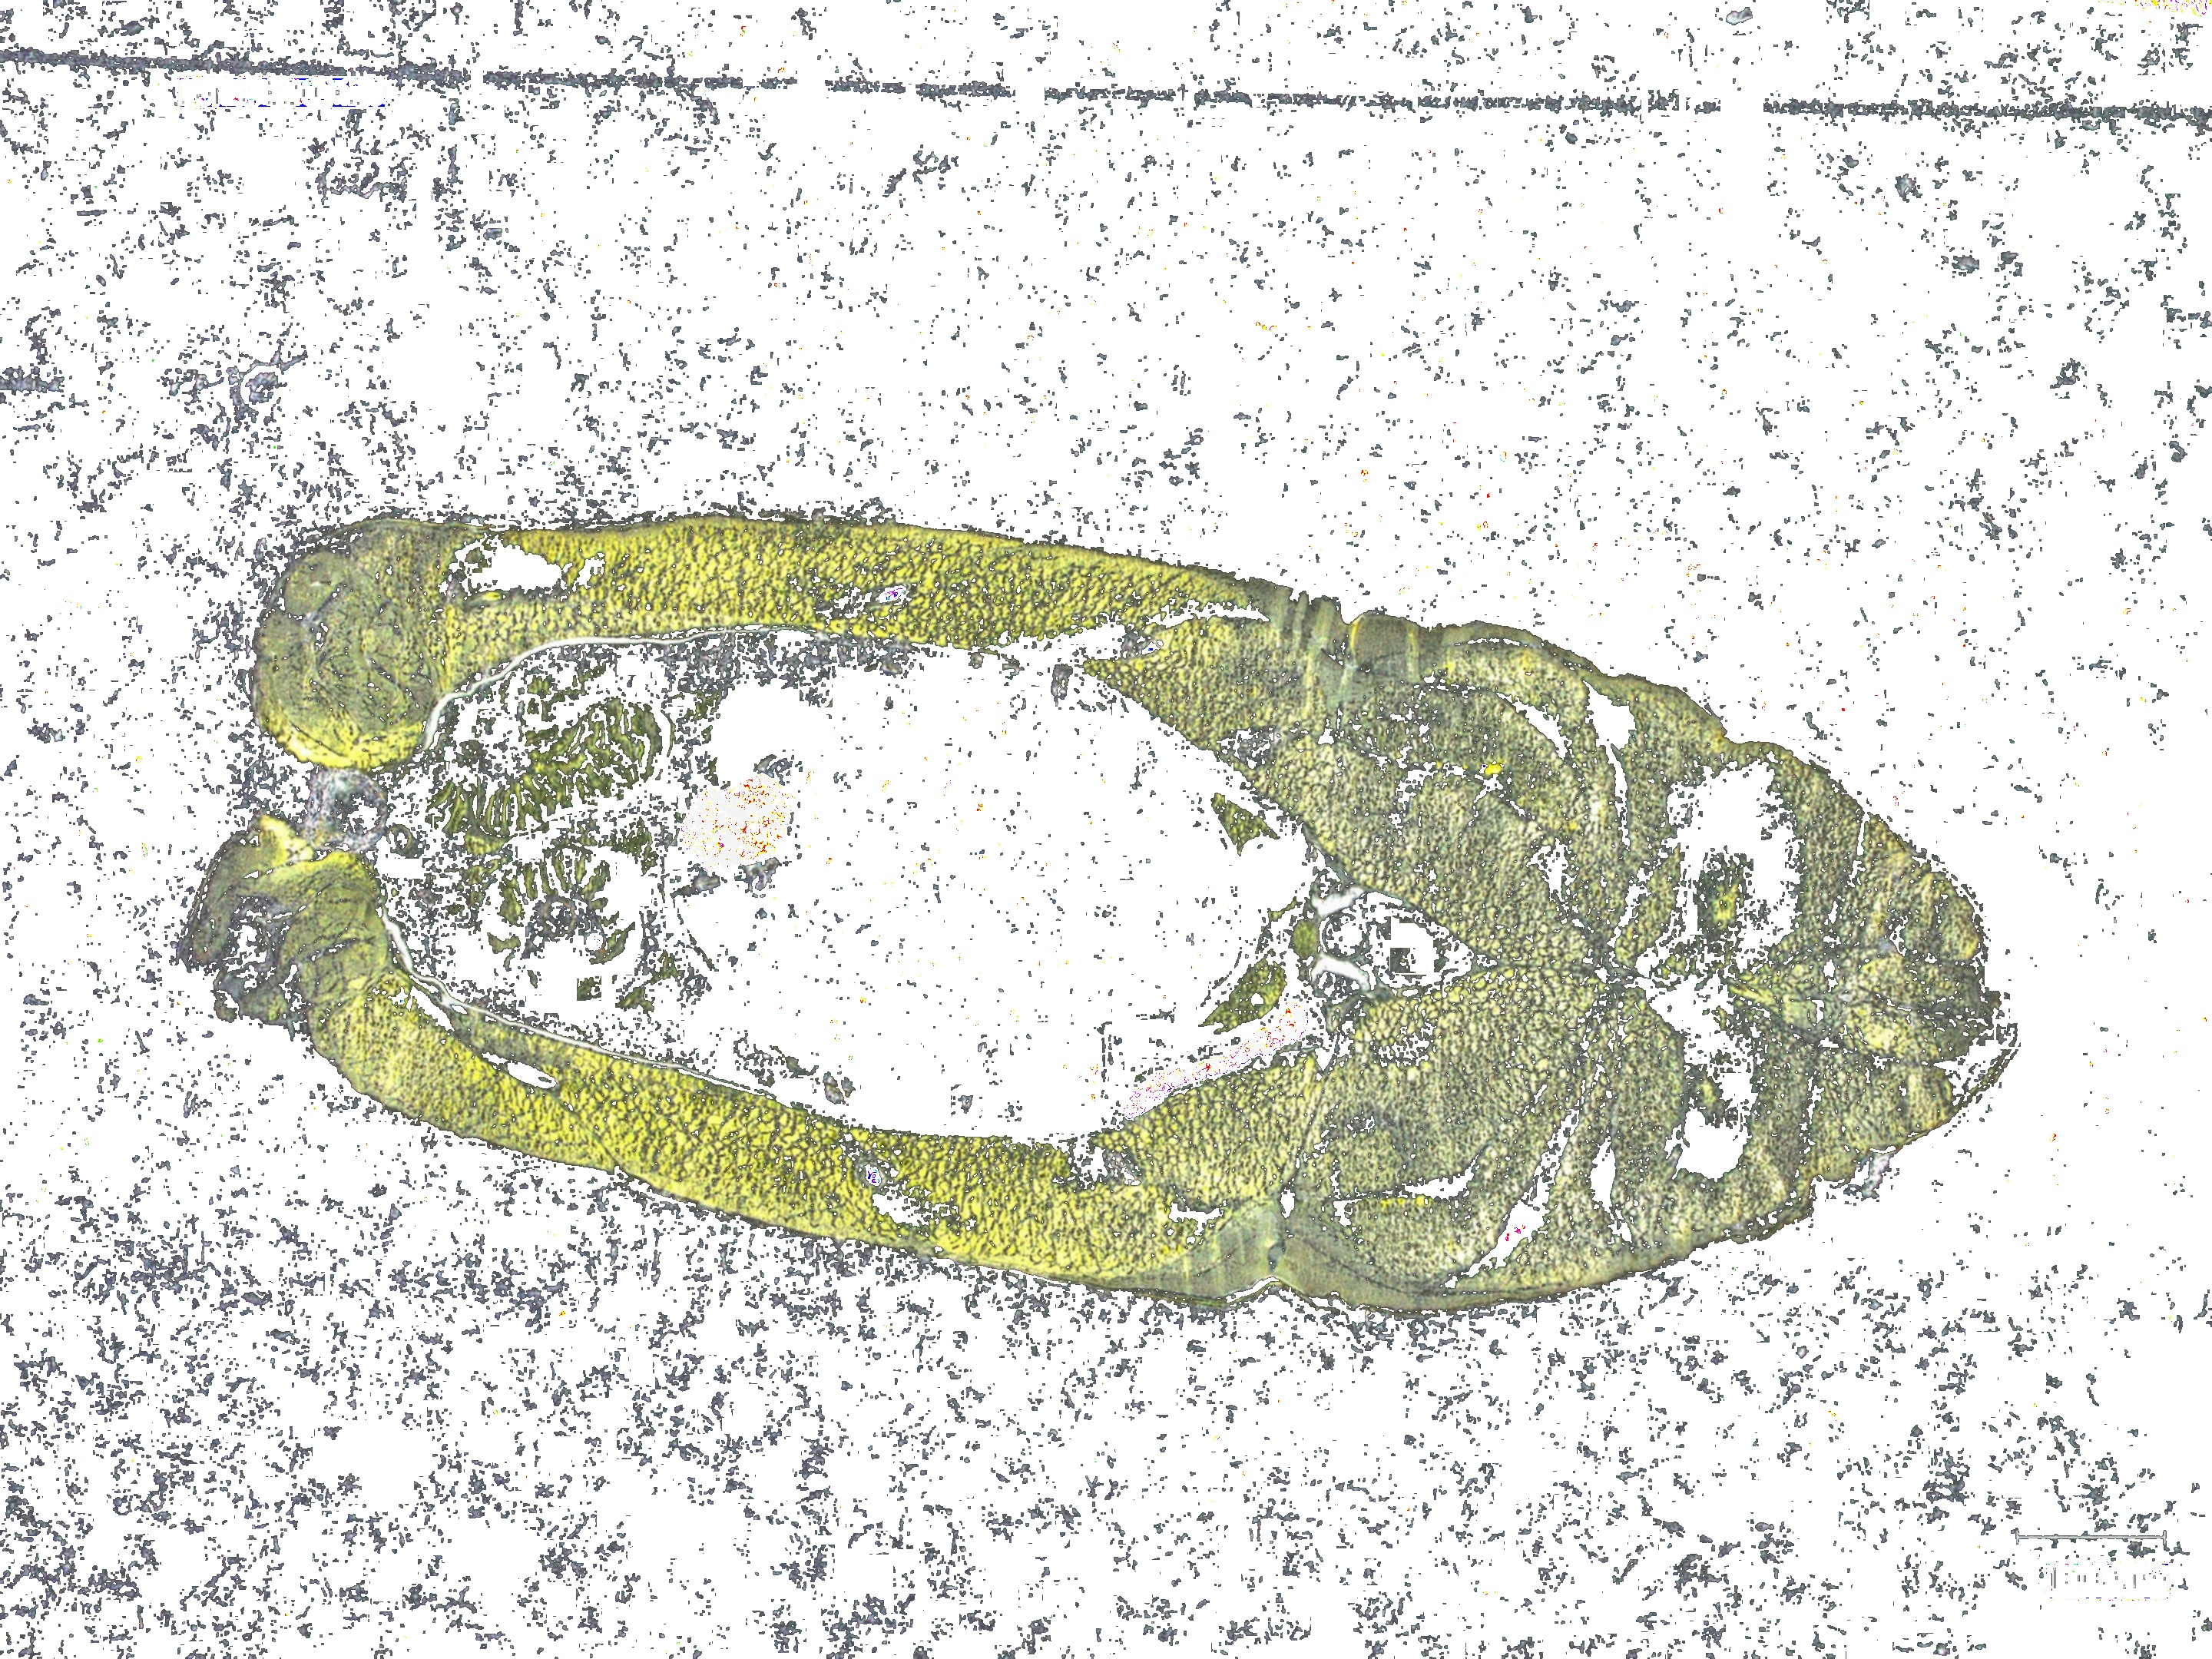
\includegraphics[width=\textwidth]{./fig/threshold/final.jpg}
        \caption{移除黑色块后的最终图像}
        \label{fig:mask}
    \end{minipage}
    \begin{minipage}{0.4\textwidth}
        \centering
        \includegraphics[width=\textwidth]{./fig/threshold/fingerprint.jpg}
        \caption{使用指纹算法进行分割的结果}
        \label{fig:fingerprint}
    \end{minipage}
\end{figure}

这种方法展示了结合颜色增强和阈值分割技术有效地从显微图像中分割生物组织和石蜡的实用性。挑战在于准确地区分组织碎片与背景噪声和其他非组织元素。这种方法对于组织病理学中的自动图像分析特别有效,其中准确的组织分割对于研究至关重要。

\subsubsection{另一种阈值分割方法:指纹算法}
在文献回顾过程中,找到了一篇描述了基于 Otsu 算法的改进分割方法的文章,专门适用于指纹分割。考虑到组织切片和指纹都是具有复杂模式和纹理的生物组织,我们假设这种算法也可能对切片组织的分割有效。应用这种方法的结果在 \autoref{fig:fingerprint} 中进行了说明。

指纹算法是 Otsu 方法的一种改编,特别有效于区分高密度和低密度区域,这对于需要区分脊和谷的对比度的应用,如指纹识别,是理想的。在生物组织分割的背景下使用这种算法可能提供一种强大的方式来划定样本内不同细胞密度或结构的区域。

\subsubsection{总结}

基于讨论的图像预处理技术,边缘检测和阈值分割在突出生物组织的特征和消除石蜡干扰方面都显示出了有希望的结果。这些预处理步骤显著增强了关键特征的可见性,同时最小化了噪声和无关信息,这对于组织病理学中的准确分析至关重要。

为了利用这些改进,可以建立三个数据集:

\begin{itemize}
    \item 通过 \textbf{边缘检测} 处理的图像。
    \item 通过 \textbf{阈值分割} 处理的图像。
    \item 使用 \textbf{指纹算法} 处理的图像。
\end{itemize}

这些数据集将作为即将进行的模型训练阶段的训练集。利用多样的预处理方法不仅增强了模型的鲁棒性,通过提供数据的多样表示,而且有助于探索哪种图像预处理技术最能有效地帮助模型学习相关特征。

\subsection{模型 2:使用简单 CNN 网络的预处理图像}

在本节中,我们将模型 1c(从前面的实验中表现最好的模型)调整为使用预处理图像。架构保持不变;然而,输入现在由经过各种预处理技术的图像组成:

\begin{itemize}
    \item \textbf{模型 2a:} 使用经过 Canny 边缘检测处理的图像。
    \item \textbf{模型 2b:} 使用经过阈值分割处理的图像。
    \item \textbf{模型 2c:} 输入是使用指纹算法分割的图像。
\end{itemize}

每个模型都遵循模型 1c 的架构,包括每个具有 32 个特征图和 3x3 内核的三个卷积层,最大池化层,以及一个具有 256 个神经元的全连接层。

结果显示在下面的图中(\autoref{fig:model22_acc} 和 \autoref{fig:model22_loss}),展示了模型 2a、2b 和 2c 的训练和验证准确率以及损失。
\begin{figure}
    \centering
    \begin{minipage}{0.49\textwidth}
        \centering
        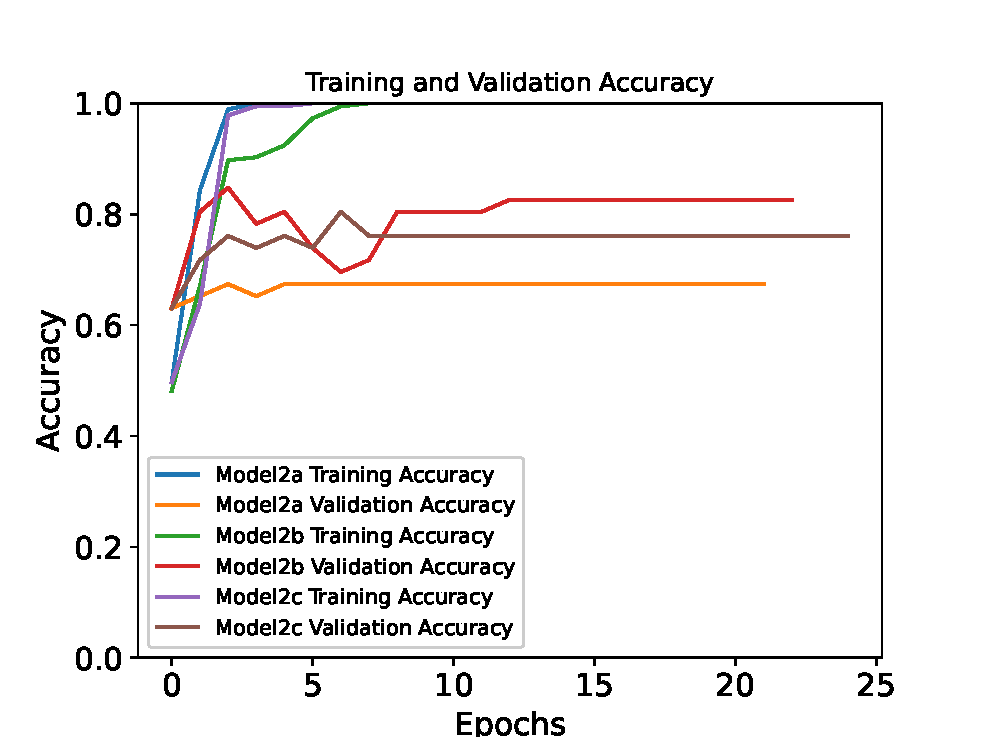
\includegraphics[width=\textwidth]{./fig/model2/accuracy22.eps}
        \caption{模型 2 的准确率}
        \label{fig:model22_acc}
    \end{minipage}
    \begin{minipage}{0.49\textwidth}
        \centering
        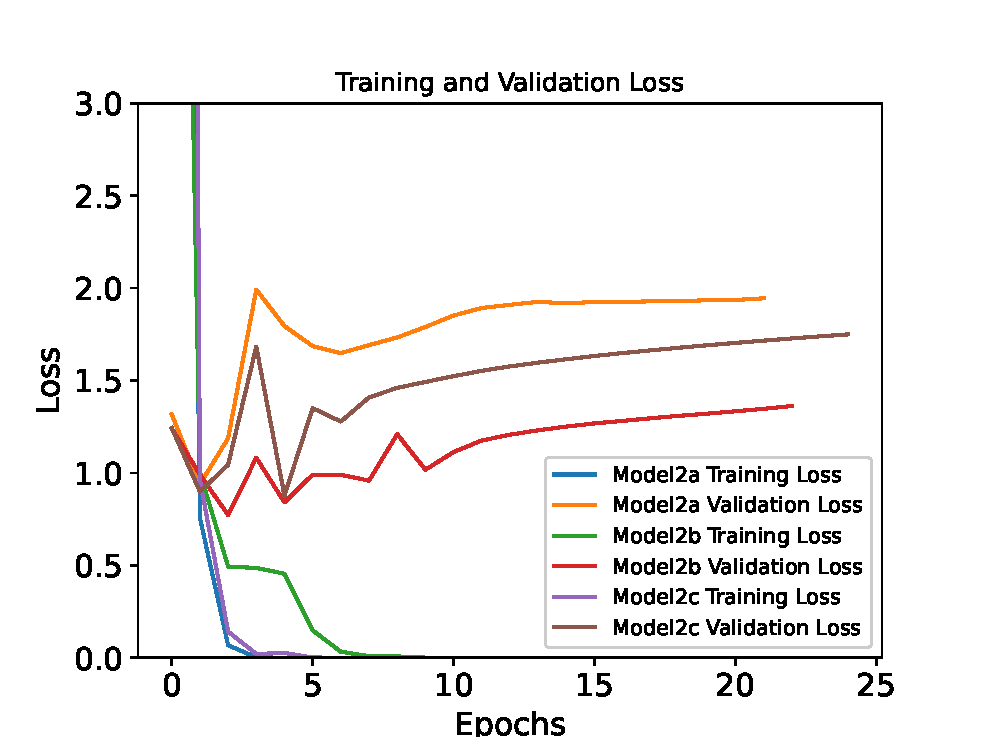
\includegraphics[width=\textwidth]{./fig/model2/loss22.eps}
        \caption{模型 2 的损失}
        \label{fig:model22_loss}
    \end{minipage}
\end{figure}


\subsubsection{小结}
图表显示,模型 2a 和 2c 在大约 8 个训练周期后开始稳定,训练准确率接近 100\%,而验证准确率分别稳定在 65\% 和 75\% 左右。尽管准确率高,但这两个模型的验证损失都相对较高,超过 1,这表明过拟合和对未见过的数据的泛化能力有限。

然而,模型 2b 在大约 10 个训练周期后收敛,显示出最高的验证准确率,约为 82\%,并且损失在 1 和 1.2 之间波动。这表明模型 2b 在验证集上的表现更好,表明更好的适应性和鲁棒性。这可能是因为模型 2b 处理的是彩色图像,这些图像从 RGB 通道提供了更丰富的特征,可能增强了特征提取和泛化能力。

然而,有一种风险是在预处理步骤中可能会丢失重要的细节,特别是在模型 2b 的阈值分割中。这可能会对模型在特定类型的图像上的性能产生负面影响。以下是这种关键信息丢失的一个例子:

\begin{figure}
    \centering
    \begin{minipage}{0.45\textwidth}
        \centering
        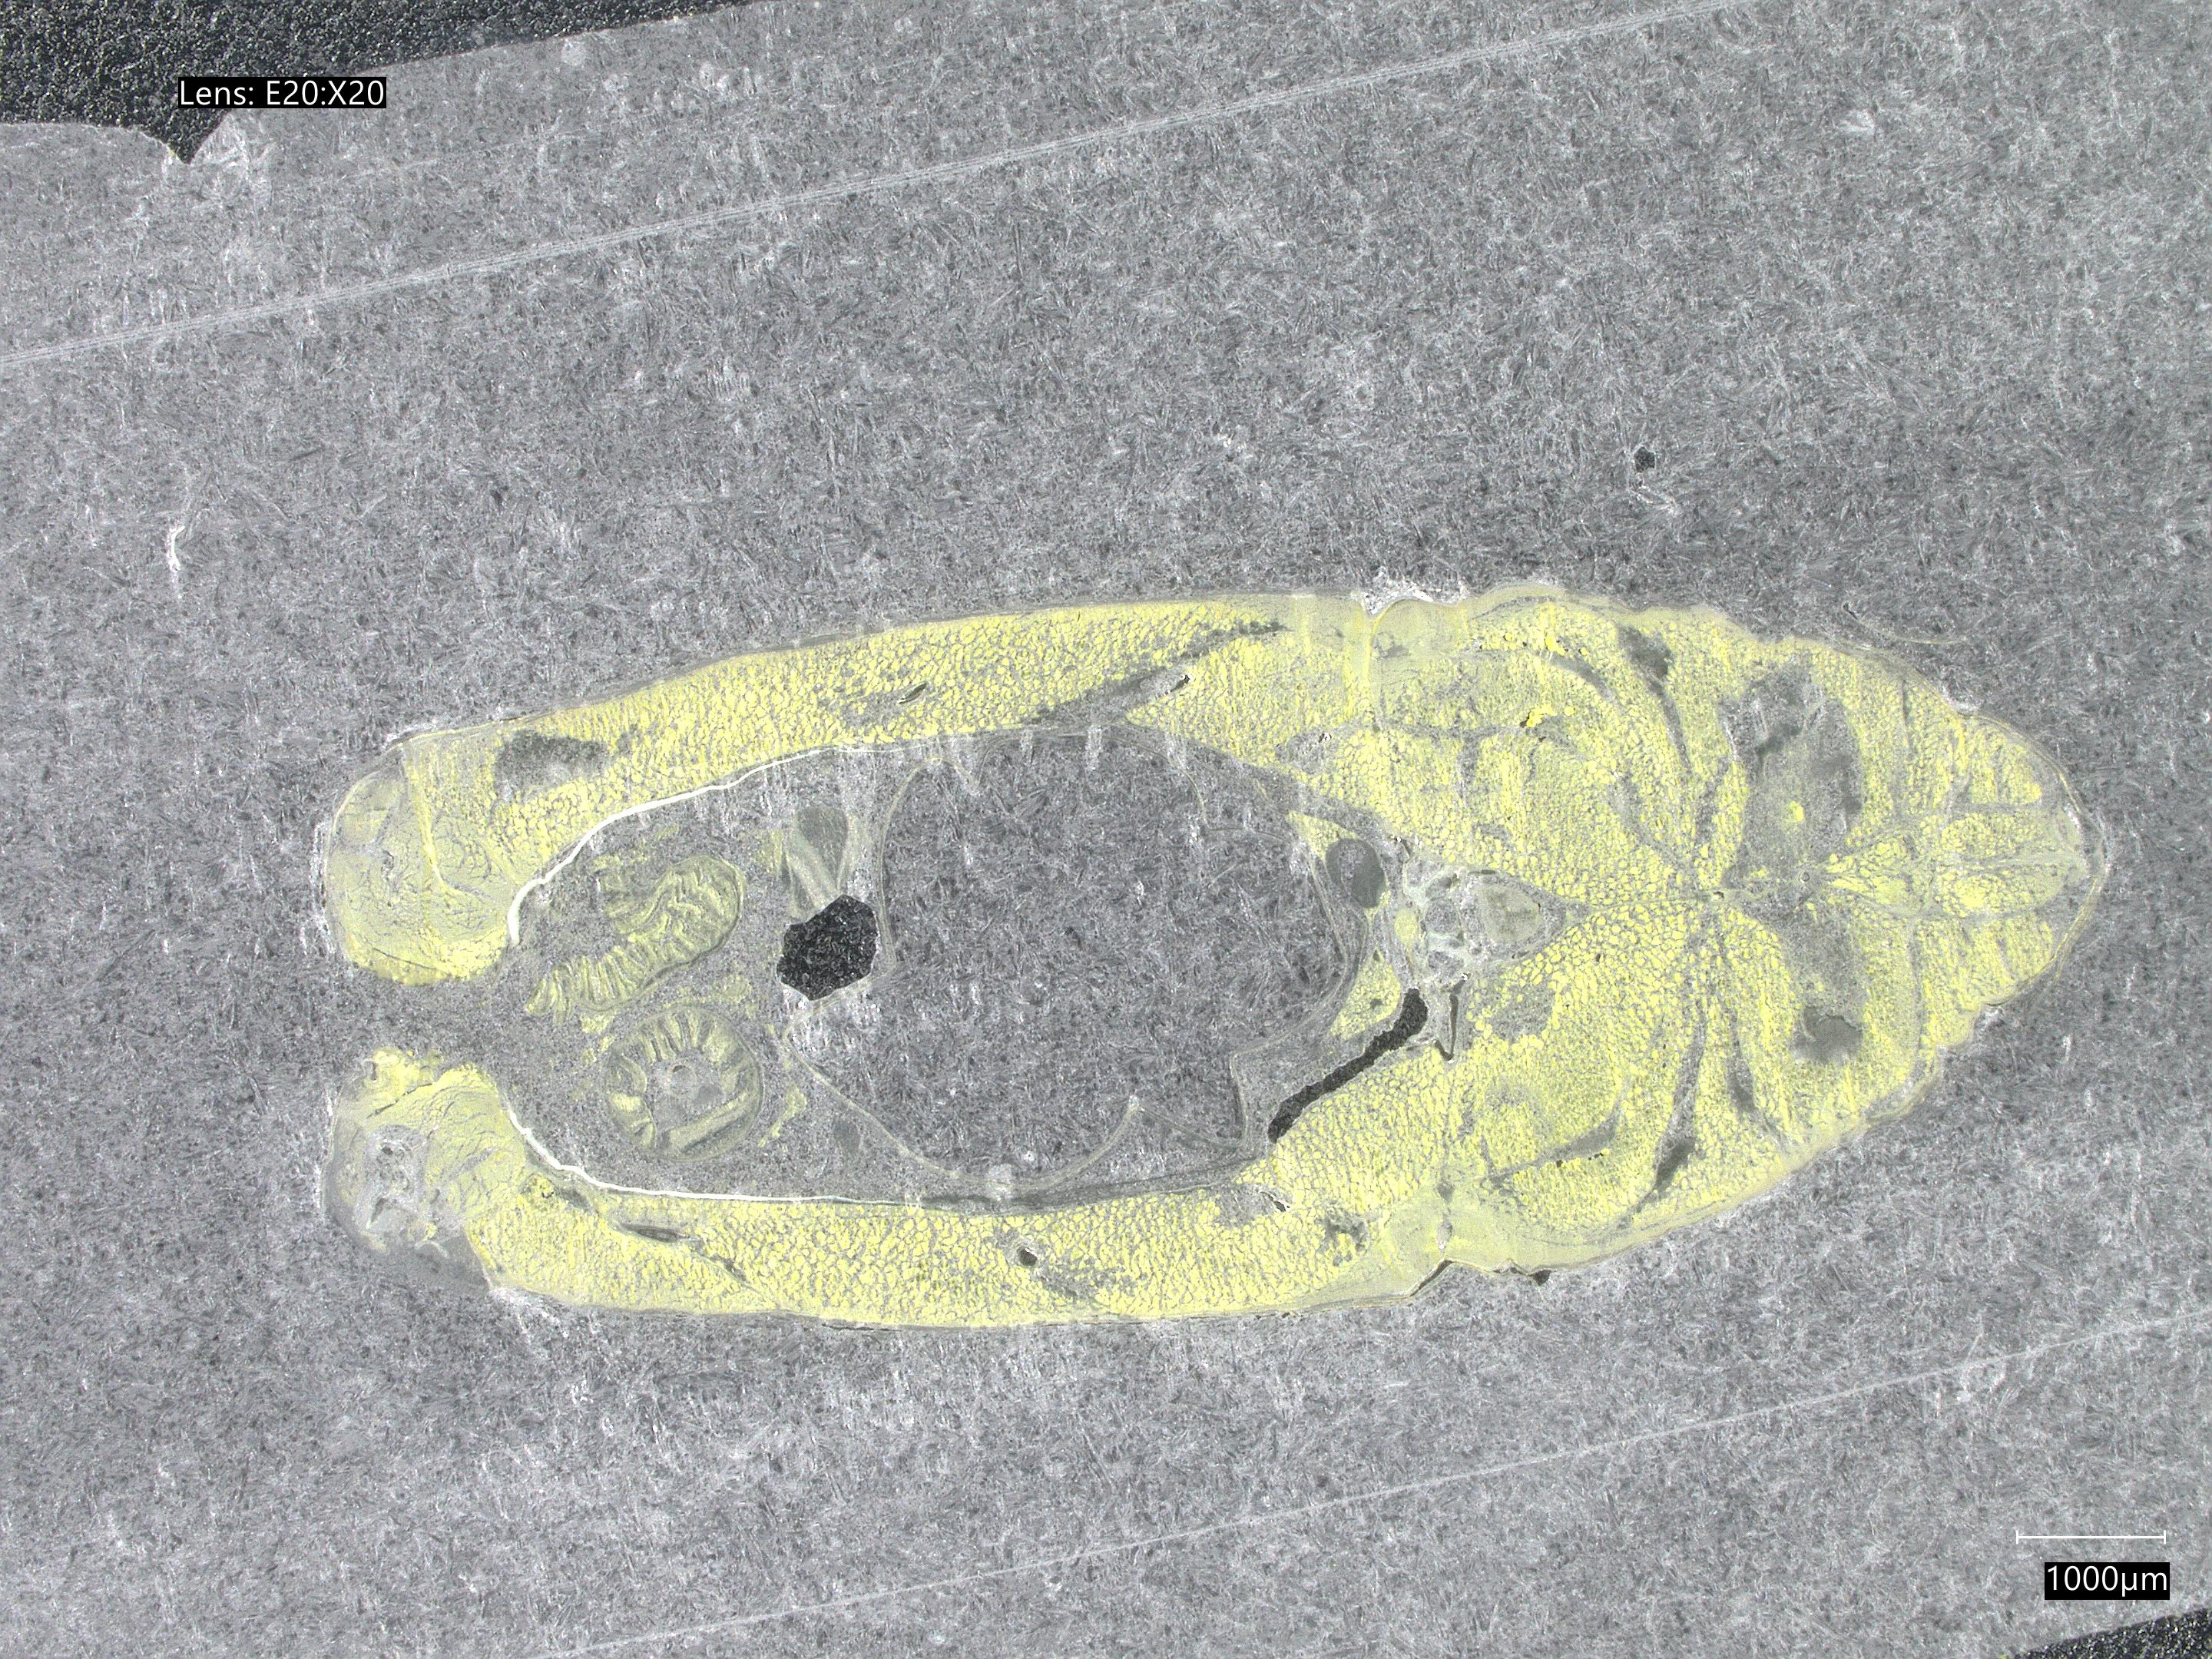
\includegraphics[width=\textwidth]{./fig/model2/origin20240205_161427.jpg}
        \caption{原始图像}
        \label{fig:origin}
    \end{minipage}
    \begin{minipage}{0.45\textwidth}
        \centering
        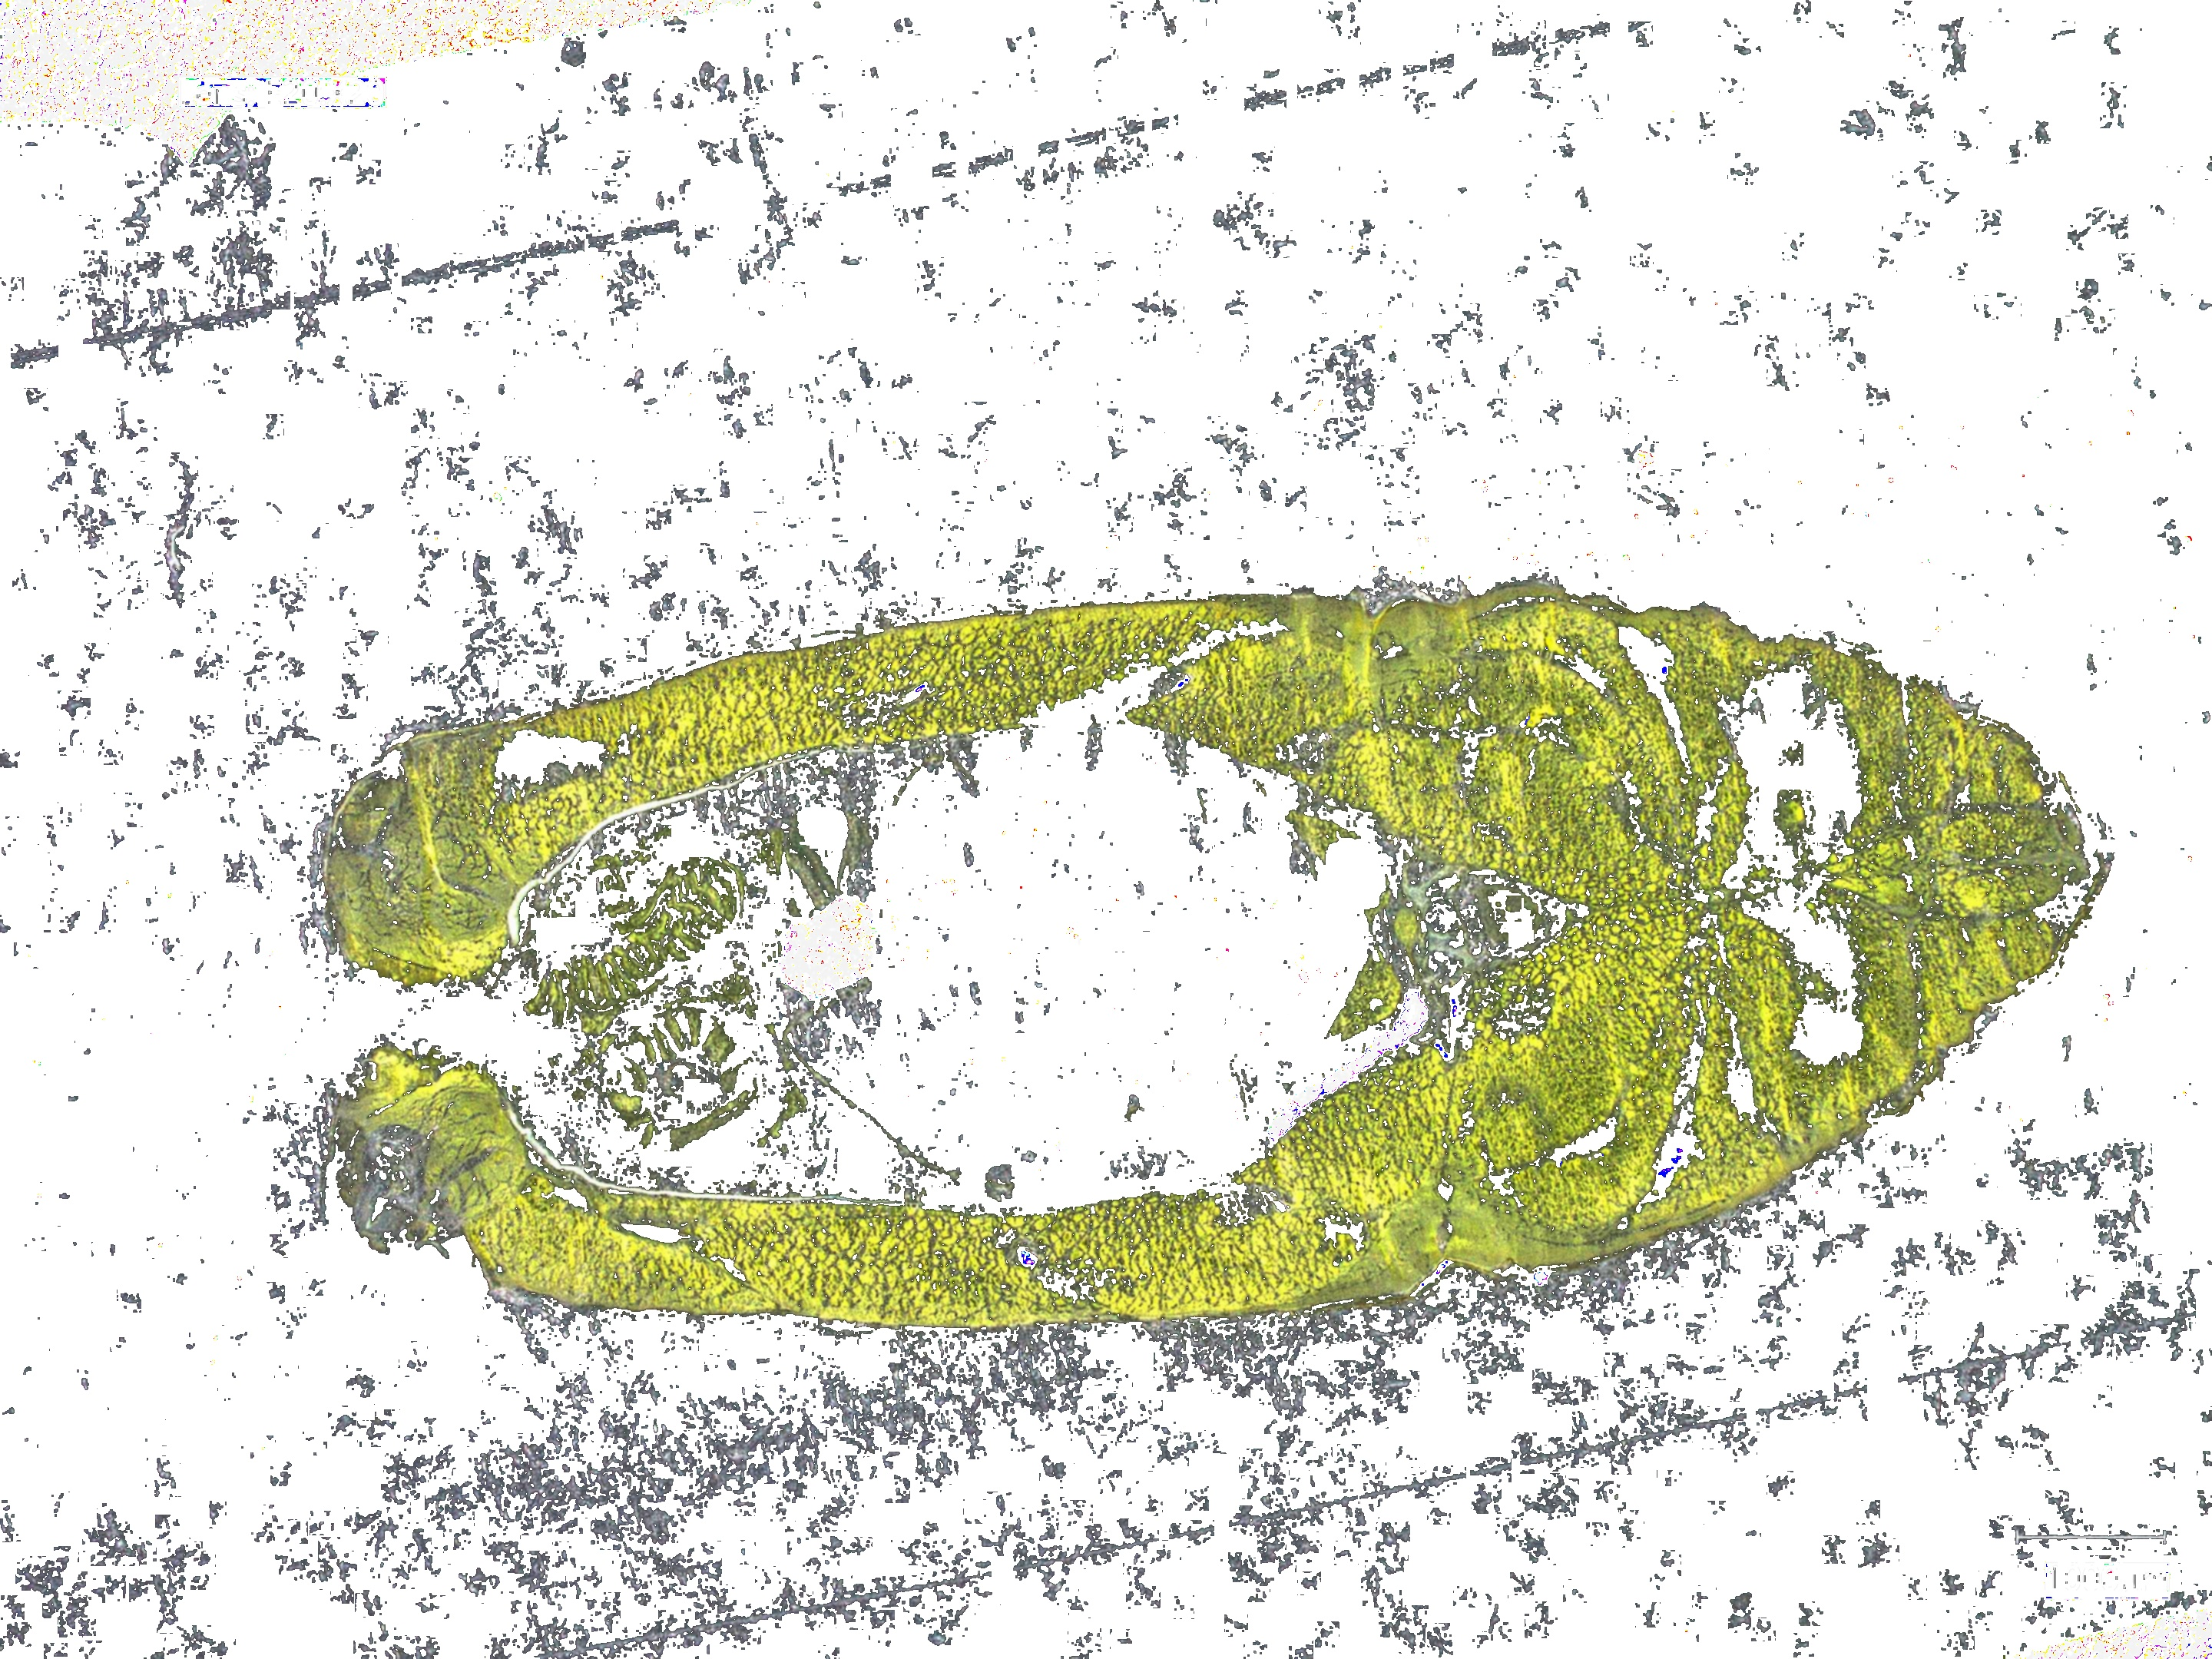
\includegraphics[width=\textwidth]{./fig/model2/yellow20240205_161427.jpg}
        \caption{黄色阈值分割后的图像}
        \label{fig:yellow}
    \end{minipage}
\end{figure}

在 \autoref{fig:yellow} 中,我们看到模型 2b 的训练集中使用的阈值分割算法显著增强了水平褶皱,可能在训练过程中使模型混淆。

这些发现突显了图像预处理的挑战。过度的预处理有时会消除关键信息,导致训练结果降低。在未来的步骤中,可能会采用迁移学习,使用适应我们数据集的预训练的大规模深度学习模型,以提高训练效果并解决这些挑战。

\subsection{模型 3:原始图像与迁移学习}

\textbf{使用预训练模型的迁移学习}

我们正在整合三个在 ImageNet 数据集上预训练的知名模型:VGG16、VGG19 和 InceptionV3。这些模型带有预训练的权重,这些权重经过高度优化,预计在适应我们特定的数据集时,将显著提高特征提取能力。

\begin{itemize}
    \item VGG16(模型 3a)和 VGG19(模型 3b)相似,但 VGG19 有三个额外的卷积层,可能提供更好的特征提取能力。
    \item InceptionV3(模型 3c)整合了 Inception 模块,使其能够在多个尺度上捕获更广泛的特征,提供更复杂且可能更有效的特征提取机制。
\end{itemize}

\textbf{迁移学习的适应性}

为了防止过拟合并优化迁移学习过程:

\begin{itemize}
    \item 使用了早停法。
    \item 学习率设定较低,对于 VGG16 和 VGG19 为 1e-5,对于结构更复杂的 InceptionV3 稍高,为 1e-4。
    \item 所有模型都被调整为接受 224x224 的输入大小,除了 InceptionV3 使用其默认的输入大小 299x299。这种统一的输入大小有助于标准化数据预处理步骤。
    \item 在每个模型的基础模型层之后添加了一个全局平均池化层,然后是一个与输出类别数匹配的全连接层。
\end{itemize}

\textbf{模型训练的观察}

以下是这些模型的训练和验证性能:

\begin{figure}[H]
    \centering
    \begin{minipage}{0.49\textwidth}
        \centering
        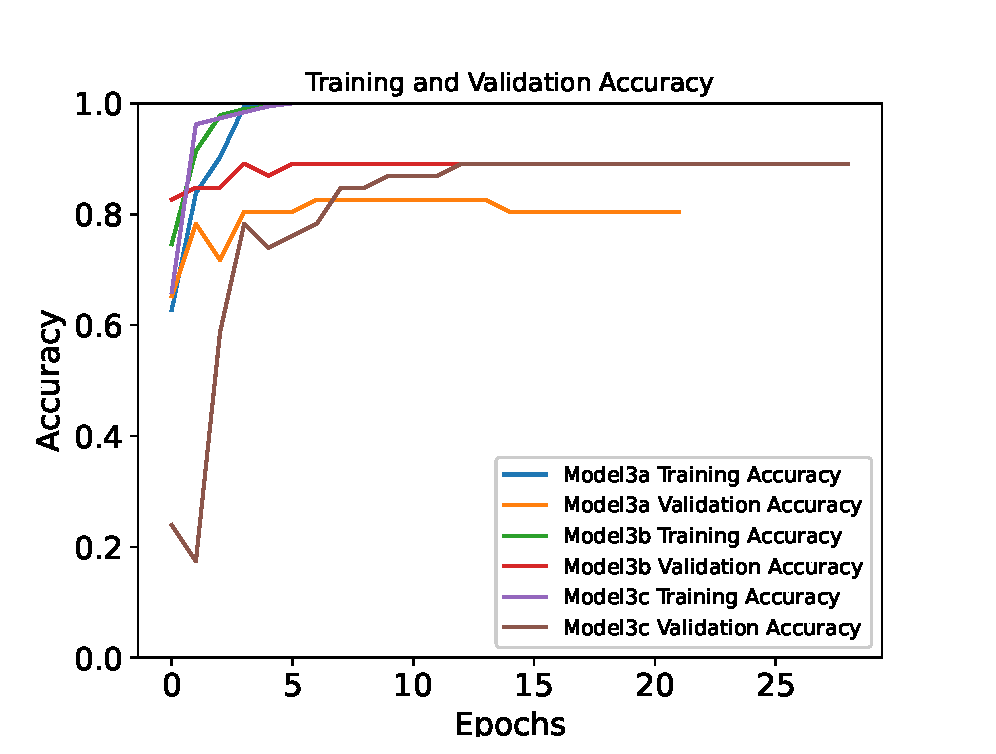
\includegraphics[width=\textwidth]{./fig/model3/accuracy33.eps}
        \caption{模型 3 的准确率}
        \label{fig:model33_acc}
    \end{minipage}
    \begin{minipage}{0.49\textwidth}
        \centering
        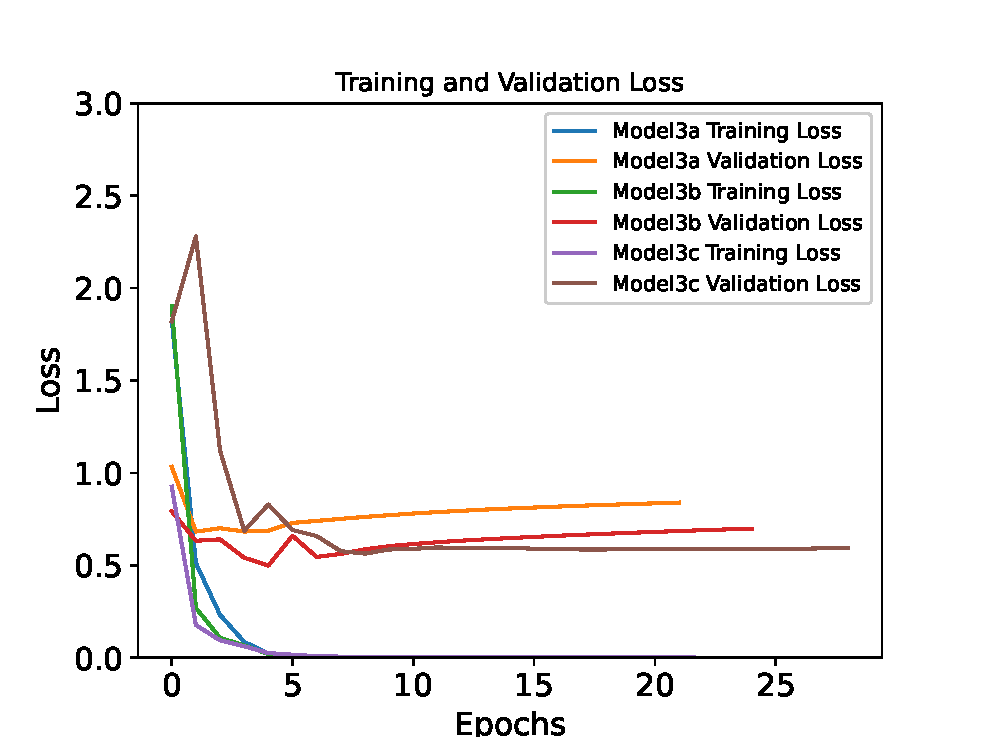
\includegraphics[width=\textwidth]{./fig/model3/loss33.eps}
        \caption{模型 3 的损失}
        \label{fig:model33_loss}
    \end{minipage}
\end{figure}

\textbf{分析}
\begin{itemize}
    \item 模型 3b(VGG19)和 3c(InceptionV3)显示出约 90\% 的显著更高的验证准确率,与模型 3a(VGG16)相比。
    \item 损失指标表明,模型 3c(InceptionV3)在三者中具有最低的验证损失,表明它在泛化到未见过的数据方面最为有效。这突显了 InceptionV3 在捕获复杂特征方面的优越能力。
    \item 模型 3a 和模型 3b 之间的性能差距支持了这样的观点,即 VGG19 中额外的卷积层增强了其比 VGG16 更有效地处理图像特征的能力。
\end{itemize}

\subsubsection{小结}

对 VGG16、VGG19 和 InceptionV3 模型的比较分析显示,InceptionV3 提供了最佳的训练结果,其训练和验证准确率分别收敛于 1 和 0.9 左右,损失收敛于 0.6。这表明 InceptionV3 模型不仅有效地进行训练,而且展示了优越的泛化能力。

\subsection{模型选择总结}
当在模型系列——模型 1、模型 2 和模型 3——之间进行比较时,显然模型 3 的表现最好,特别是模型 3c。其根本原因可能是由于模型 3 基于在大规模图像数据集上预训练的深度卷积网络,使得特征提取更有效,能够开发出强大的特征空间。

\textbf{模型 3c(InceptionV3)的显著特性:}

\begin{itemize}
    \item \textbf{架构设计:} InceptionV3 具有模块化设计,包含多个 "inception 模块",这些模块包括在同一层内并行操作的多尺度卷积层。这种模块化方法使网络能够在各种尺度和深度上捕获广泛的特征。
    \item \textbf{特征提取:} Inception 模块可以通过在同一层内处理不同尺度的特征来适应性地捕获适当的特征表示。这种适应性使其特别适合处理复杂的图像数据,如生物医学图像。
    \item \textbf{深度网络处理:} InceptionV3 集成了批量归一化和残差连接,这些在训练深度网络中至关重要。这些技术有效地缓解了梯度消失的问题,从而有助于训练更深的模型而不降低性能。
\end{itemize}

考虑到这些优点,模型 3c(InceptionV3)被选为我们的最终模型,用于进一步的应用和测试。这个模型不仅因其先进的架构创新而突出,而且因其在泛化到新的、未见过的数据方面的证明效果而突出,使其非常适合复杂的任务,如医学图像分析,其中准确性和可靠性至关重要。
